
%Futuring Study material template- This template is designed for the soft copy
%This template is for the subject PHYSICS ONLY
%----------------------------------------------------------------------------------------
%	PACKAGES AND OTHER DOCUMENT CONFIGURATIONS
%----------------------------------------------------------------------------------------

\documentclass[11pt,twoside]{book} % Default font size and left-justified equations

%%%
%----------------------------------------------------------------------------------------
%	VARIOUS REQUIRED PACKAGES AND CONFIGURATIONS
%----------------------------------------------------------------------------------------
\usepackage{eucal}
\usepackage{setspace}
\usepackage{bigints}
\usepackage{etoolbox}
\usepackage{dirtytalk}
\usepackage{epigraph}
\usepackage{physics}
\usepackage{amssymb}
\usepackage{chemfig}
\usepackage{stackrel}
\usepackage{scalerel}
\usepackage{longtable}
\usepackage{tabularx}
\usepackage{caption}
\usepackage{multirow}
\usepackage{environ}
\usepackage{subfigure}
\usepackage{graphicx} % Required for including pictures
\graphicspath{{Pictures/}{Pictures/sketching/}{Pictures/single and complex/}{Pictures/Coordinate system/}{Pictures/vector/}{Pictures/jamfigure/}{Pictures/conicsection/}{Pictures/conicsection/}{Pictures/electrostatics/}{Pictures/LCR/} {Pictures/BHU/}{Pictures/HCU/}{Pictures/Jest/}{Pictures/magnetostatics/}{Pictures/p-coulombs law/}{Pictures/p-vector/}{Pictures/quantum/}{Pictures/}{Pictures/BHU/}{Pictures/HCU/}{Pictures/JEST/} {Pictures/STR/}{Pictures/nuclear/} {Pictures/quantum/} {Pictures/Particle/} {Pictures/Newtons law/} {Pictures/work and energy/} {Pictures/Kinematics/}{Pictures/math prelim/} {Pictures/semiconductors/}{Pictures/Fluid mechanics/}{Pictures/Bipolar junction transistor/}{Pictures/Solid state/}{Pictures/digital/}{Pictures/Waves/}{Pictures/OPAMP/}{Pictures/Optics/}{Pictures/Wave Optics/}{Pictures/Net/}{Pictures/NET/}{Pictures/Gate/}{pictures/Newtons law/}{pictures/Kinematics/}{pictures/work and energy/}{pictures/jamfigure/}{Pictures/Problems/} {Pictures/Dirac delta function/}{Pictures/Differential equations/}{Pictures/Assignment/}{Pictures/Assignments/}
{Pictures/Electronics-CSIR/} {Pictures/CM/} {Pictures/Statistical Physics/}{Pictures/Digital Electronics/}{Pictures/Relativity and Electromagnetism/}{Pictures/Net 2019/}}
 % Specifies the directory where pictures are stored
\usepackage{float}
\usepackage{lipsum} % Inserts dummy text
\usepackage{wrapfig}
\usepackage{tikz} % Required for drawing custom shapes
\usepackage{amsmath}
 % English language/hyphenation

\usepackage{enumitem}
\newlist{questions}{enumerate}{3}
\setlist[questions]{wide=0pt, leftmargin=15pt, labelwidth=15pt, labelsep=0pt, align=left,label=\color{futuringtheme}\bfseries\large\arabic*.}
\newcommand{\question}{\item}


%\AtBeginEnvironment{enumerate}{\linespread{6.84}\selectfont}

 
 
\NewEnviron{abox}{%
	\begin{center}
\begin{tikzpicture}
\node[align=center,anchor=base,draw,rectangle,text width=\textwidth,line width=2pt,rounded corners=15pt,draw=ocre,fill=white,fill opacity=0.9,inner sep=10pt] 
{\centering \textbf{ \huge \color{futuringtheme}\BODY}};
\end{tikzpicture}

	\end{center}
	
	
}
\newcommand{\exyear}[1]{\newline \llap{}\hfill \color{futuringtheme}{\textbf{[#1]}}}
\usepackage{booktabs} % Required for nicer horizontal rules in tables
\usepackage{tasks}
\usepackage{xcolor} % Required for specifying colors by name
\definecolor{ocre}{RGB}{243,102,25} % Define the orange color used for highlighting throughout the book
\definecolor{futuringtheme}{RGB}{0,142,212}
%----------------------------------------------------------------------------------------
%..............................Added packages
\usepackage{import}
\usepackage{array}
\usepackage{colortbl}
\usepackage{cutwin}

\usepackage[printwatermark]{xwatermark}

\newsavebox\mylogobox
\savebox\mylogobox{\tikz[opacity=0.2]\node[inner sep=0pt] (russell) at (0,0)
	{
\includegraphics[width=3cm]{../Config/Pictures/logotra2.png}};}
\newwatermark*[
allpages,
angle=0,
scale=5,
xpos=0,
ypos=0
]{\usebox\mylogobox}



%.........................
%	MARGINS
%----------------------------------------------------------------------------------------
\usepackage{tasks}
\usepackage{geometry} % ccbyRequired for adjusting page dimensions and margins

\geometry{
	paper=a4paper, % Paper size, change to letterpaper for US letter size
	top=2cm, % Top margin
	bottom=2cm, % Bottom margin
	left=2cm, % Left margin
	right=2cm, % Right margin
	headheight=14pt, % Header height
	footskip=1.4cm, % Space from the bottom margin to the baseline of the footer
	headsep=10pt, % Space from the top margin to the baseline of the header
	%showframe, % Uncomment to show how the type block is set on the page
}

\allowdisplaybreaks
\makeatletter
\def\SetTotalwidth{\advance\linewidth by \@totalleftmargin
	\@totalleftmargin=0pt}
\makeatother

%----------------------------------------------------------------------------------------
%y

\usepackage{avant} % Use the Avantgarde font for headings
%\usepackage{times} % Use the Times font for headings
\usepackage{mathptmx} % Use the Adobe Times Roman as the default text font together with math symbols from the Sym­bol, Chancery and Com­puter Modern fonts

\usepackage{microtype} % Slightly tweak font spacing for aesthetics
\usepackage[utf8]{inputenc} % Required for including letters with accents
\usepackage[T1]{fontenc} % Use 8-bit encoding that has 256 glyphs

%----------------------------------------------------------------------------------------
%	BIBLIOGRAPHY AND INDEX
%----------------------------------------------------------------------------------------


%----------------------------------------------------------------------------------------
%	MAIN TABLE OF CONTENTS
%----------------------------------------------------------------------------------------

\usepackage{titletoc} % Required for manipulating the table of contents

\contentsmargin{0cm} % Removes the default margin

% Part text styling (this is mostly taken care of in the PART HEADINGS section of this file)
\titlecontents{part}
	[0cm] % Left indentation
	{\addvspace{20pt}\bfseries} % Spacing and font options for parts
	{}
	{}
	{}

% Chapter text styling
\titlecontents{chapter}
	[1.25cm] % Left indentation
	{\addvspace{12pt}\large\sffamily\bfseries} % Spacing and font options for chapters
	{\color{ocre!60}\contentslabel[\Large\thecontentslabel]{1.25cm}\color{ocre}} % Formatting of numbered sections of this type
	{\color{ocre}} % Formatting of numberless sections of this type
	{\color{ocre!60}\normalsize\;\titlerule*[.5pc]{.}\;\thecontentspage} % Formatting of the filler to the right of the heading and the page number

% Section text styling
\titlecontents{section}
	[1.25cm] % Left indentation
	{\addvspace{3pt}\sffamily\bfseries} % Spacing and font options for sections
	{\contentslabel[\thecontentslabel]{1.25cm}} % Formatting of numbered sections of this type
	{} % Formatting of numberless sections of this type
	{\hfill\color{black}\thecontentspage} % Formatting of the filler to the right of the heading and the page number

% Subsection text styling
\titlecontents{subsection}
	[1.25cm] % Left indentation
	{\addvspace{1pt}\sffamily\small} % Spacing and font options for subsections
	{\contentslabel[\thecontentslabel]{1.25cm}} % Formatting of numbered sections of this type
	{} % Formatting of numberless sections of this type
	{\ \titlerule*[.5pc]{.}\;\thecontentspage} % Formatting of the filler to the right of the heading and the page number

% Figure text styling
\titlecontents{figure}
	[1.25cm] % Left indentation
	{\addvspace{1pt}\sffamily\small} % Spacing and font options for figures
	{\thecontentslabel\hspace*{1em}} % Formatting of numbered sections of this type
	{} % Formatting of numberless sections of this type
	{\ \titlerule*[.5pc]{.}\;\thecontentspage} % Formatting of the filler to the right of the heading and the page number

% Table text styling
\titlecontents{table}
	[1.25cm] % Left indentation
	{\addvspace{1pt}\sffamily\small} % Spacing and font options for tables
	{\thecontentslabel\hspace*{1em}} % Formatting of numbered sections of this type
	{} % Formatting of numberless sections of this type
	{\ \titlerule*[.5pc]{.}\;\thecontentspage} % Formatting of the filler to the right of the heading and the page number

%----------------------------------------------------------------------------------------
%	MINI TABLE OF CONTENTS IN PART HEADS
%----------------------------------------------------------------------------------------

% Chapter text styling
\titlecontents{lchapter}
	[0em] % Left indentation
	{\addvspace{15pt}\large\sffamily\bfseries} % Spacing and font options for chapters
	{\color{ocre}\contentslabel[\Large\thecontentslabel]{1.25cm}\color{ocre}} % Chapter number
	{}  
	{\color{ocre}\normalsize\sffamily\bfseries\;\titlerule*[.5pc]{.}\;\thecontentspage} % Page number

% Section text styling
\titlecontents{lsection}
	[0em] % Left indentation
	{\sffamily\small} % Spacing and font options for sections
	{\contentslabel[\thecontentslabel]{1.25cm}} % Section number
	{}
	{}

% Subsection text styling (note these aren't shown by default, display them by searchings this file for tocdepth and reading the commented text)
\titlecontents{lsubsection}
	[.5em] % Left indentation
	{\sffamily\footnotesize} % Spacing and font options for subsections
	{\contentslabel[\thecontentslabel]{1.25cm}}
	{}
	{}

%----------------------------------------------------------------------------------------
%	HEADERS AND FOOTERS
%----------------------------------------------------------------------------------------

\usepackage{fancyhdr} % Required for header and footer configuration

\pagestyle{fancy} % Enable the custom headers and footers

\renewcommand{\chaptermark}[1]{\markboth{\sffamily\normalsize\bfseries\chaptername\ \thechapter.\ #1}{}} % Styling for the current chapter in the header
\renewcommand{\sectionmark}[1]{\markright{\sffamily\normalsize\thesection\hspace{5pt}#1}{}} % Styling for the current section in the header

\fancyhf{} % Clear default headers and footers
\fancyhead[LE,RO]{\sffamily\normalsize\thepage} % Styling for the page number in the header
\fancyhead[LO]{\rightmark} % Print the nearest section name on the left side of odd pages
\fancyhead[RE]{\leftmark} % Print the current chapter name on the right side of even pages
\renewcommand{\headrulewidth}{0.5pt} % Thickness of the rule under the header


% Removes the header from odd empty pages at the end of chapters
\makeatletter
\renewcommand{\cleardoublepage}{
\clearpage\ifodd\c@page\else
\hbox{}
\vspace*{\fill}
\thispagestyle{empty}
\newpage
\fi}


\fancypagestyle{plain}{% Redefine plain pages tyle
	\fancyhf{}% Clear header/footer
	
	\fancyhead[LE,RO]{\sffamily\normalsize\thepage}
	 % Print the nearest section name on the left side of odd pages
	\fancyhead[RE]{\leftmark}
}

%----------------------------------------------------------------------------------------

%Box Styles
\usepackage{tcolorbox}
\newtcolorbox{myboxthree}{colback=futuringtheme!5!white,colframe=ocre!75}






















%	THEOREM STYLES
%----------------------------------------------------------------------------------------

\usepackage{amsmath,amsfonts,amssymb,amsthm} % For math equations, theorems, symbols, etc

\newcommand{\intoo}[2]{\mathopen{]}#1\,;#2\mathclose{[}}
\newcommand{\ud}{\mathop{\mathrm{{}d}}\mathopen{}}
\newcommand{\intff}[2]{\mathopen{[}#1\,;#2\mathclose{]}}
\renewcommand{\qedsymbol}{$\blacksquare$}
\newtheorem{notation}{Notation}[chapter]

% Boxed/framed environments
\newtheoremstyle{ocrenumbox}% Theorem style name
{0pt}% Space above
{0pt}% Space below
{\normalfont}% Body font
{}% Indent amount
{\small\bf\sffamily\color{ocre}}% Theorem head font
{\;}% Punctuation after theorem head
{0.25em}% Space after theorem head
{\small\sffamily\color{ocre}\thmname{#1}\nobreakspace\thmnumber{\@ifnotempty{#1}{}\@upn{#2}}% Theorem text (e.g. Theorem 2.1)
\thmnote{\nobreakspace\the\thm@notefont\sffamily\bfseries\color{black}---\nobreakspace#3.}} % Optional theorem note

\newtheoremstyle{blacknumex}% Theorem style name
{5pt}% Space above
{5pt}% Space below
{\normalfont}% Body font
{} % Indent amount
{\small\bf\sffamily}% Theorem head font
{\;}% Punctuation after theorem head
{0.25em}% Space after theorem head
{\small\sffamily{\tiny\ensuremath{\blacksquare}}\nobreakspace\thmname{#1}\nobreakspace\thmnumber{\@ifnotempty{#1}{}\@upn{#2}}% Theorem text (e.g. Theorem 2.1)
\thmnote{\nobreakspace\the\thm@notefont\sffamily\bfseries---\nobreakspace#3.}}% Optional theorem note

\newtheoremstyle{blacknumbox} % Theorem style name
{0pt}% Space above
{0pt}% Space below
{\normalfont}% Body font
{}% Indent amount
{\small\bf\sffamily}% Theorem head font
{\;}% Punctuation after theorem head
{0.25em}% Space after theorem head
{\small\sffamily\thmname{#1}\nobreakspace\thmnumber{\@ifnotempty{#1}{}\@upn{#2}}% Theorem text (e.g. Theorem 2.1)
\thmnote{\nobreakspace\the\thm@notefont\sffamily\bfseries---\nobreakspace#3.}}% Optional theorem note

% Non-boxed/non-framed environments
\newtheoremstyle{ocrenum}% Theorem style name
{5pt}% Space above
{5pt}% Space below
{\normalfont}% Body font
{}% Indent amount
{\small\bf\sffamily\color{ocre}}% Theorem head font
{\;}% Punctuation after theorem head
{0.25em}% Space after theorem head
{\small\sffamily\color{ocre}\thmname{#1}\nobreakspace\thmnumber{\@ifnotempty{#1}{}\@upn{#2}}% Theorem text (e.g. Theorem 2.1)
\thmnote{\nobreakspace\the\thm@notefont\sffamily\bfseries\color{black}---\nobreakspace#3.}} % Optional theorem note
\makeatother

%Box style for Solution environment
\newtheoremstyle{solbox}% Theorem style name
{0pt}% Space above
{0pt}% Space below
{\normalfont}% Body font
{}% Indent amount
{\small\bf\sffamily\color{ocre}}% Theorem head font
{\;}% Punctuation after theorem head
{0.25em}% Space after theorem head
{\small\sffamily\color{ocre}Solution:}


% Defines the theorem text style for each type of theorem to one of the three styles above
\newcounter{dummy} 
\numberwithin{dummy}{section}
\theoremstyle{ocrenumbox}
\newtheorem{theoremeT}[dummy]{Theorem}
\newtheorem{problem}{Problem}[chapter]
\newtheorem{exerciseT}{Exercise}[chapter]
\theoremstyle{blacknumex}
\newtheorem{exampleT}{Example}[chapter]
\theoremstyle{blacknumbox}
\newtheorem{vocabulary}{Vocabulary}[chapter]
\newtheorem{definitionT}{Definition}[section]
\newtheorem{corollaryT}[dummy]{Corollary}
\theoremstyle{ocrenum}
\newtheorem{proposition}[dummy]{Proposition}
\theoremstyle{solbox}
\newtheorem{answerT}[dummy]{Solution}

%----------------------------------------------------------------------------------------
%	DEFINITION OF COLORED BOXES
%----------------------------------------------------------------------------------------

\RequirePackage[framemethod=default]{mdframed} % Required for creating the theorem, definition, exercise and corollary boxes

% Theorem box
\newmdenv[skipabove=7pt,
skipbelow=7pt,
backgroundcolor=white,
linecolor=ocre,
innerleftmargin=5pt,
innerrightmargin=5pt,
innertopmargin=10pt,
leftmargin=0cm,
rightmargin=0cm,
innerbottommargin=5pt]{tBox}

% Exercise box	  
\newmdenv[skipabove=7pt,
skipbelow=7pt,
rightline=false,
leftline=true,
topline=false,
bottomline=false,
backgroundcolor=ocre!10,
linecolor=ocre,
innerleftmargin=5pt,
innerrightmargin=5pt,
innertopmargin=5pt,
innerbottommargin=5pt,
leftmargin=0cm,
rightmargin=0cm,
linewidth=4pt]{eBox}	

% Definition box
\newmdenv[skipabove=7pt,
skipbelow=7pt,
rightline=false,
leftline=true,
topline=false,
bottomline=false,
linecolor=ocre,
innerleftmargin=5pt,
innerrightmargin=5pt,
innertopmargin=0pt,
leftmargin=0cm,
rightmargin=0cm,
linewidth=4pt,
innerbottommargin=0pt]{dBox}	

% Corollary box
\newmdenv[skipabove=7pt,
skipbelow=7pt,
rightline=false,
leftline=true,
topline=false,
bottomline=false,
linecolor=gray,
backgroundcolor=black!5,
innerleftmargin=5pt,
innerrightmargin=5pt,
innertopmargin=5pt,
leftmargin=0cm,
rightmargin=0cm,
linewidth=4pt,
innerbottommargin=5pt]{cBox}

% Creates an environment for each type of theorem and assigns it a theorem text style from the "Theorem Styles" section above and a colored box from above
\newenvironment{theorem}{\begin{tBox}\begin{theoremeT}}{\end{theoremeT}\end{tBox}}
\newenvironment{exercise}{\begin{eBox}\begin{exerciseT}}{\hfill{\color{ocre}\tiny\ensuremath{\blacksquare}}\end{exerciseT}\end{eBox}}				  
\newenvironment{definition}{\begin{dBox}\begin{definitionT}}{\end{definitionT}\end{dBox}}	
\newenvironment{example}{\begin{exampleT}}{\hfill{\tiny\ensuremath{\blacksquare}}\end{exampleT}}		
\newenvironment{corollary}{\begin{cBox}\begin{corollaryT}}{\end{corollaryT}\end{cBox}}	
\newenvironment{answer}{\begin{tBox}\begin{answerT}}{\end{answerT}\end{tBox}}	

%----------------------------------------------------------------------------------------
%	REMARK ENVIRONMENT
%----------------------------------------------------------------------------------------

\newenvironment{remark}{\par\vspace{10pt}\normlasize % Vertical white space above the remark and smaller font size
\begin{list}{}{
\leftmargin=35pt % Indentation on the left
\rightmargin=25pt}\item\ignorespaces % Indentation on the right
\makebox[-2.5pt]{\begin{tikzpicture}[overlay]
\node[draw=ocre!60,line width=1pt,circle,fill=ocre!25,font=\sffamily\bfseries,inner sep=2pt,outer sep=0pt] at (-15pt,0pt){\textcolor{ocre}{R}};\end{tikzpicture}} % Orange R in a circle
\advance\baselineskip -1pt}{\end{list}\vskip5pt} % Tighter line spacing and white space after remark

\newenvironment{note}{\par\vspace{10pt}\normalsize % Vertical white space above the remark and smaller font size
	\begin{list}{}{
			\leftmargin=35pt % Indentation on the left
			\rightmargin=25pt}\item\ignorespaces % Indentation on the right
		\makebox[-2.5pt]{\begin{tikzpicture}[overlay]
			\node[draw=ocre!60,line width=1pt,rectangle,fill=ocre!25,font=\sffamily\bfseries,inner sep=2pt,outer sep=0pt] at (-15pt,0pt){\textcolor{ocre}{Note}};\end{tikzpicture}} % Orange R in a circle
		\advance\baselineskip -5pt}{\end{list}\vskip5pt} % Tighter line spacing and white space after remark

%----------------------------------------------------------------------------------------
%	SECTION NUMBERING IN THE MARGIN
%----------------------------------------------------------------------------------------

\makeatletter
\renewcommand{\@seccntformat}[1]{\llap{\textcolor{ocre}{\csname the#1\endcsname}\hspace{1em}}}                    
\renewcommand{\section}{\@startsection{section}{1}{\z@}
{-4ex \@plus -1ex \@minus -.4ex}
{1ex \@plus.2ex }
{\normalfont\large\sffamily\bfseries}}
\renewcommand{\subsection}{\@startsection {subsection}{2}{\z@}
{-3ex \@plus -0.1ex \@minus -.4ex}
{0.5ex \@plus.2ex }
{\normalfont\sffamily\bfseries}}
\renewcommand{\subsubsection}{\@startsection {subsubsection}{3}{\z@}
{-2ex \@plus -0.1ex \@minus -.2ex}
{.2ex \@plus.2ex }
{\normalfont\small\sffamily\bfseries}}                        
\renewcommand\paragraph{\@startsection{paragraph}{4}{\z@}
{-2ex \@plus-.2ex \@minus .2ex}
{.1ex}
{\normalfont\small\sffamily\bfseries}}

%----------------------------------------------------------------------------------------
%	PART HEADINGS
%----------------------------------------------------------------------------------------

% Numbered part in the table of contents
\newcommand{\@mypartnumtocformat}[2]{%
	\setlength\fboxsep{0pt}%
	\noindent\colorbox{ocre!20}{\strut\parbox[c][.7cm]{\ecart}{\color{ocre!70}\Large\sffamily\bfseries\centering#1}}\hskip\esp\colorbox{ocre!40}{\strut\parbox[c][.7cm]{\linewidth-\ecart-\esp}{\Large\sffamily\centering#2}}%
}

% Unnumbered part in the table of contents
\newcommand{\@myparttocformat}[1]{%
	\setlength\fboxsep{0pt}%
	\noindent\colorbox{ocre!40}{\strut\parbox[c][.7cm]{\linewidth}{\Large\sffamily\centering#1}}%
}

\newlength\esp
\setlength\esp{4pt}
\newlength\ecart
\setlength\ecart{1.2cm-\esp}
\newcommand{\thepartimage}{}%
\newcommand{\partimage}[1]{\renewcommand{\thepartimage}{#1}}%
\def\@part[#1]#2{%
\ifnum \c@secnumdepth >-2\relax%
\refstepcounter{part}%
\addcontentsline{toc}{part}{\texorpdfstring{\protect\@mypartnumtocformat{\thepart}{#1}}{\partname~\thepart\ ---\ #1}}
\else%
\addcontentsline{toc}{part}{\texorpdfstring{\protect\@myparttocformat{#1}}{#1}}%
\fi%
\startcontents%
\markboth{}{}%
{\thispagestyle{empty}%
\begin{tikzpicture}[remember picture,overlay]%
\node at (current page.north west){\begin{tikzpicture}[remember picture,overlay]%	
\fill[ocre!20](0cm,0cm) rectangle (\paperwidth,-\paperheight);
\node[anchor=north] at (4cm,-3.25cm){\color{ocre!40}\fontsize{220}{100}\sffamily\bfseries\thepart}; 
\node[anchor=south east] at (\paperwidth-1cm,-\paperheight+1cm){\parbox[t][][t]{8.5cm}{
\printcontents{l}{0}{\setcounter{tocdepth}{1}}% The depth to which the Part mini table of contents displays headings; 0 for chapters only, 1 for chapters and sections and 2 for chapters, sections and subsections
}};
\node[anchor=north east] at (\paperwidth-1.5cm,-3.25cm){\parbox[t][][t]{15cm}{\strut\raggedleft\color{white}\fontsize{30}{30}\sffamily\bfseries#2}};
\end{tikzpicture}};
\end{tikzpicture}}%
\@endpart}
\def\@spart#1{%
\startcontents%
\phantomsection
{\thispagestyle{empty}%
\begin{tikzpicture}[remember picture,overlay]%
\node at (current page.north west){\begin{tikzpicture}[remember picture,overlay]%	
\fill[ocre!20](0cm,0cm) rectangle (\paperwidth,-\paperheight);
\node[anchor=north east] at (\paperwidth-1.5cm,-3.25cm){\parbox[t][][t]{15cm}{\strut\raggedleft\color{white}\fontsize{30}{30}\sffamily\bfseries#1}};
\end{tikzpicture}};
\end{tikzpicture}}
\addcontentsline{toc}{part}{\texorpdfstring{%
\setlength\fboxsep{0pt}%
\noindent\protect\colorbox{ocre!40}{\strut\protect\parbox[c][.7cm]{\linewidth}{\Large\sffamily\protect\centering #1\quad\mbox{}}}}{#1}}%
\@endpart}
\def\@endpart{\vfil\newpage
\if@twoside
\if@openright
\null
\thispagestyle{empty}%
\newpage
\fi
\fi
\if@tempswa
\twocolumn
\fi}

%----------------------------------------------------------------------------------------
%	CHAPTER HEADINGS
%----------------------------------------------------------------------------------------

% A switch to conditionally include a picture, implemented by Christian Hupfer
\newif\ifusechapterimage
\usechapterimagetrue
\newcommand{\thechapterimage}{}%
\newcommand{\chapterimage}[1]{\ifusechapterimage\renewcommand{\thechapterimage}{#1}\fi}%
\newcommand{\autodot}{.}
\def\@makechapterhead#1{%
{\parindent \z@ \raggedright \normalfont
\ifnum \c@secnumdepth >\m@ne
\if@mainmatter
\begin{tikzpicture}[remember picture,overlay]
\node at (current page.north west)
{\begin{tikzpicture}[remember picture,overlay]
\node[anchor=north west,inner sep=0pt] at (0,0) {\ifusechapterimage\includegraphics[width=\paperwidth]{\thechapterimage}\fi};
\draw[anchor=west] (\Gm@lmargin,-9cm) node [line width=2pt,rounded corners=15pt,draw=ocre,fill=white,fill opacity=0.5,inner sep=15pt]{\strut\makebox[22cm]{}};
\draw[anchor=west] (\Gm@lmargin+.3cm,-9cm) node {\huge\sffamily\bfseries\color{black}\thechapter\autodot~#1\strut};
\end{tikzpicture}};
\end{tikzpicture}
\else
\begin{tikzpicture}[remember picture,overlay]
\node at (current page.north west)
{\begin{tikzpicture}[remember picture,overlay]
\node[anchor=north west,inner sep=0pt] at (0,0) {\ifusechapterimage\includegraphics[width=\paperwidth]{\thechapterimage}\fi};
\draw[anchor=west] (\Gm@lmargin,-9cm) node [line width=2pt,rounded corners=15pt,draw=ocre,fill=white,fill opacity=0.5,inner sep=15pt]{\strut\makebox[22cm]{}};
\draw[anchor=west] (\Gm@lmargin+.3cm,-9cm) node {\huge\sffamily\bfseries\color{black}#1\strut};
\end{tikzpicture}};
\end{tikzpicture}
\fi\fi\par\vspace*{270\p@}}}

%-------------------------------------------

\def\@makeschapterhead#1{%
\begin{tikzpicture}[remember picture,overlay]
\node at (current page.north west)
{\begin{tikzpicture}[remember picture,overlay]
\node[anchor=north west,inner sep=0pt] at (0,0) {\ifusechapterimage\includegraphics[width=\paperwidth]{\thechapterimage}\fi};
\draw[anchor=west] (\Gm@lmargin,-9cm) node [line width=2pt,rounded corners=15pt,draw=ocre,fill=white,fill opacity=0.5,inner sep=15pt]{\strut\makebox[22cm]{}};
\draw[anchor=west] (\Gm@lmargin+.3cm,-9cm) node {\huge\sffamily\bfseries\color{black}#1\strut};
\end{tikzpicture}};
\end{tikzpicture}
\par\vspace*{270\p@}}
\makeatother

%----------------------------------------------------------------------------------------
%	LINKS
%----------------------------------------------------------------------------------------

\usepackage{hyperref}
\hypersetup{hidelinks,backref=true,pagebackref=true,hyperindex=true,colorlinks=false,breaklinks=true,urlcolor=ocre,bookmarks=true,bookmarksopen=false}

\usepackage{bookmark}
\bookmarksetup{
open,
numbered,
addtohook={%
\ifnum\bookmarkget{level}=0 % chapter
\bookmarksetup{bold}%
\fi
\ifnum\bookmarkget{level}=-1 % part
\bookmarksetup{color=ocre,bold}%
\fi
}
}
 % Insert the commands.tex file which contains the majority of the structure behind the template

\hypersetup{pdftitle={Title},pdfauthor={Futuring}} % Uncomment and fill out to include PDF metadata for the author and title of the book

%----------------------------------------------------------------------------------------

\begin{document}
\chapterimage{../../Config/Pictures/one.jpg}
%----------------------------------------------------------------------------------------
%	TITLE PAGE
%----------------------------------------------------------------------------------------

%Place the content from the snippet file titlepage and fill out the details -- Titlepage details
%----------------------------------------------------------------------------------------
%	COPYRIGHT PAGE
%----------------------------------------------------------------------------------------

%Place the content from the snippet file copyrightpage and fill out the details -- copyright details

%----------------------------------------------------------------------------------------
%	TABLE OF CONTENTS
%----------------------------------------------------------------------------------------



%----------------------------------------------------------------------------------------
%	CHAPTER 1
%----------------------------------------------------------------------------------------



%\chapter{Fourier Series}
\section{Series Expansion of Periodic Functions}
The basic fact about Fourier series is as follows.\\
If $f(x)$ is a periodic function of $x$,with a period $L$ . The \textbf{Fundamental interval} is taken to be $(a,b)$, so that $L=(b-a)$\\
Then, $f(x)=f(x+L)=f(x+nL)$ Where $n$ is any integer.\\If the function $f(x)$ also satisfies a set of conditions known as \textbf{Drichlet's  Conditions} given as below\\

\begin{enumerate}
	\item It is single-valued in the interval $(a, b)$
	\item It is bounded in the interval $(a, b)$
	\item It has at most a finite number of maxima and minima in the interval $(a, b)$
	\item It has only a finite number of discontinuity in the interval $(a, b)$
\end{enumerate}
\begin{theorem}\label{geneq}
	Then such a function can be expressed by a sum of a set  sine and cosine functions (or complex exponentials). This series is known as \textbf{Fourier Series Expansion}\index{Fourier Series}.\\
	\begin{equation}
	\begin{array}{c}
	f(x)=\frac{a_{0}}{2}+\sum_{n=1}^{\infty} a_{n} \cos \frac{2n \pi x}{L}+\sum_{n=1}^{\infty} b_{n} \sin \frac{2n \pi x}{L}
	\end{array}
	\end{equation}
	
	$a_{0}, a_{n}, b_{n}$ are constants, known as Fourier co-efficients.
	\begin{equation}
	a_{0}=\frac{2}{b-a} \int_{a}^{b} f(x) d x
	\end{equation}
	\begin{equation}
	a_{n}=\frac{2}{b-a} \int_{a}^{b} f(x) \cdot \cos \left(\frac{2 n \pi x}{b-a}\right) d x
	\end{equation}
	\begin{equation}
	b_{n}=\frac{2}{b-a} \int_{a}^{b} f(x) \cdot \sin \left(\frac{2 n \pi x}{b-a}\right) d x
	\end{equation}
\end{theorem}
The Fourier expansion of a periodic function $f(x)$ consists of the following term
\begin{enumerate}
	\item $a_{0}: a$ constant term or $D .$ C. term
	\item $a_{1} \cos \frac{\pi x}{L}$ and $b_{1} \sin \frac{\pi x}{L}:$ Fundamental frequency term i.e term having lowest frequency
	\item $a_{2} \cos \frac{2 \pi x}{L}, a_{3} \cos \frac{3 \pi x}{L} \ldots \ldots ., b_{2} \sin \frac{2 \pi x}{L}, b_{3} \sin \frac{3 \pi x}{L} \ldots \ldots .$ Overtones i.e terms having
	frequencies integer multiple of fundamental frequency term.
\end{enumerate}

\subsection{Simplified formulas when $b-a=2\pi$}

We have established the Euler formulas for a function having period $L$ and principal interval $(a,b)$.The formulas connected with fourier series expansion look a bit simpler if one choose the fundamental interval to be $(-\pi,\pi)$ or $(0,2\pi)$, ie Period $L=2\pi$.\\For the case $b-a=2\pi$, the Euler formulas become

	
\begin{theorem}\label{pareq}


\begin{equation}
a_{0}=\frac{1}{\pi} \int_{a}^{b} f(x) d x
\end{equation}
\begin{equation}
a_{0n}=\frac{1}{\pi} \int_{a}^{b} f(x) \cdot \cos n x d x
\end{equation}
\begin{equation}
b_{n}=\frac{1}{\pi} \int_{a}^{b} f(x) \cdot \sin n x d x
\end{equation}
So that the Fourier expansion becomes 
\begin{equation}
f(x)=\frac{a_{0}}{2}+\sum_{n=1}^{\infty} a_{n} \cdot \cos n x+\sum_{n=1}^{\infty} b_{n} \sin n x
\end{equation}
\end{theorem}


\begin{exercise}
	 Find the Fourier series representing $$f(x)=x, \quad 0<x<2 \pi$$
\end{exercise}
\begin{answer}
Here the interval is $(0,2\pi)$ So L=$2\pi$.From theorem \ref{pareq} we have
\begin{equation}
\label{eq1}
f(x)=\frac{a_{0}}{2}+\sum_{n=1}^{\infty} a_{n} \cdot \cos n x+\sum_{n=1}^{\infty} b_{n} \sin n x
\end{equation}
$$h
\text { Hence } \begin{aligned}
a_{0} &=\frac{1}{\pi} \int_{0}^{2 \pi} f(x) d x=\frac{1}{\pi} \int_{0}^{2 \pi} x d x=\frac{1}{\pi}\left[\frac{x^{2}}{2}\right]_{0}^{2 \pi}=2 \pi \\
a_{n} &=\frac{1}{\pi} \int_{0}^{2 \pi} f(x) \cos n x d x=\frac{1}{\pi} \int_{0}^{2 \pi} x \cos n x d x \\
&=\frac{1}{\pi}\left[x \frac{\sin n x}{n}-1 \cdot\left(-\frac{\cos n x}{n^{2}}\right)\right]_{0}^{2 \pi}=\frac{1}{\pi}\left[\frac{\cos 2 n \pi}{n^{2}}-\frac{1}{n^{2}}\right]=\frac{1}{n^{2} \pi}(1-1)=0 \\
b_{n} &=\frac{1}{\pi} \int_{0}^{2 \pi} f(x) \sin n x d x=\frac{1}{\pi} \int_{0}^{2 \pi} x \sin n x d x \\
&=\frac{1}{\pi}\left[x\left(-\frac{\cos n x}{n}\right)-1 \cdot\left(\frac{-\sin n x}{n^{2}}\right)\right]_{0}^{2 \pi}=\frac{1}{\pi}\left[\frac{-2 \pi \cos 2 n \pi}{n}\right]=-\frac{2}{n}
\end{aligned}
$$
Substituting the values of $a_{0}, a_{1}, a_{2} \ldots, b_{1}, b_{2} \ldots$ in Equation \ref{eq1}, we get
$$
x=\pi-2\left[\sin x+\frac{1}{2} \sin 2 x+\frac{1}{3} \sin 3 x+\ldots\right]
$$
\end{answer}
\begin{exercise}
Given that $f(x)=x+x^{2}$ for $-\pi<x<\pi,$ find the Fourier expression of $f(x)$
\end{exercise}

\begin{answer}
	\begin{equation}
\label{eq2}
	\text { Let } x+x^{2}=\frac{a_{0}}{2}+a_{1} \cos x+a_{2} \cos 2 x+\ldots+b_{1} \sin x+b_{2} \sin 2 x+\ldots
	\end{equation}
	$\begin{aligned} a_{0} &=\frac{1}{\pi} \int_{-\pi}^{\pi} f(x) d x=\frac{1}{\pi} \int_{-\pi}^{\pi}\left(x+x^{2}\right) d x \\ &=\frac{1}{\pi}\left[\frac{x^{2}}{2}+\frac{x^{3}}{3}\right]_{-\pi}^{\pi}=\frac{1}{\pi}\left[\frac{\pi^{2}}{2}+\frac{\pi^{3}}{3}-\frac{\pi^{2}}{2}+\frac{\pi^{3}}{3}\right]=\frac{2 \pi^{2}}{3} \\ a_{n} &=\frac{1}{\pi} \int_{-\pi}^{\pi} f(x) \cos n x d x=\int_{-\pi}^{\pi}\left(x+x^{2}\right) \cos n x d x \end{aligned}$\\
	$\begin{aligned} &=\frac{1}{\pi}\left[\left(x+x^{2}\right) \frac{\sin n x}{n}-(2 x+1) \frac{(-\cos n x)}{n^{2}}+(2)\left(-\frac{\sin n x}{n^{3}}\right)\right]_{-\pi}^{\pi} \\ &=\frac{1}{\pi}\left[(2 \pi+1) \frac{\cos n \pi}{n^{2}}-(-2 \pi+1) \frac{\cos (-n \pi)}{n^{2}}\right]=\frac{1}{\pi}\left[4 \pi \frac{\cos n \pi}{n^{2}}\right]=\frac{4(-1)^{n}}{n^{2}} \\ b_{n} &=\frac{1}{\pi} \int_{-\pi}^{\pi} f(x) \sin n x d x=\frac{1}{\pi} \int_{-\pi}^{\pi}\left(x+x^{2}\right) \sin n x d x \\ &=\frac{1}{\pi}\left[\left(x+x^{2}\right)\left(-\frac{\cos n x}{n}\right)-(2 x+1)\left(\frac{-\sin n x}{n^{2}}\right)+2 \frac{\cos n x}{n^{3}}\right]_{-\pi}^{\pi} \\ &=\frac{1}{\pi}\left[-\left(\pi+\pi^{2}\right) \frac{\cos n \pi}{n}+2 \frac{\cos n \pi}{n^{3}}+\left(-\pi+\pi^{2}\right) \frac{\cos n \pi}{n}-2 \frac{\cos n \pi}{n^{3}}\right] \\ &=\frac{1}{\pi}\left[-\frac{2 \pi}{n} \cos n \pi\right]=-\frac{2}{n}(-1)^{n} \end{aligned}$\\
	Substituting the values of $a_{0}, a_{n}, b_{n},$ in Equation \ref{eq2}, we get
	\begin{equation}
	\begin{array}{r}
	x+x^{2}=\frac{\pi^{2}}{3}+4\left[-\cos x+\frac{1}{2^{2}} \cos 2 x-\frac{1}{3^{2}} \cos 3 x+\ldots\right] 
	-2\left[-\sin x+\frac{1}{2} \sin 2 x-\frac{1}{3} \sin 3 x+\ldots\right]
	\end{array}
	\end{equation}
\end{answer}
\section{Even and Odd Functions}
\subsection{Even Function}
A function $f(x)$ is said to be \textbf{even} (or \textbf{symmetric}) function if, $f(-x)=f(x)$ The graph of such a function is symmetrical with respect to $y$ -axis . Here $y$ -axis is a mirror for the reflection of the curve.
\begin{example}
	$\cos x,\sec x ,x^2$ etc

\end{example}
The area under such a curve from $-\pi$ to $\pi$ is double the area from 0 to $\pi$, ie\\
$$\quad \int_{-\pi}^{\pi} f(x) d x=2 \int_{0}^{\pi} f(x) d x$$
\subsection{Odd Function}
A function $f(x)$ is called \textbf{odd} (or \textbf{skew symmetric}) function if
$$
f(-x)=-f(x)
$$ Odd functions will be symmetric about origin.\\
Here the area under the curve from $-\pi$ to $\pi$ is zero.
$$
\int_{-\pi}^{\pi} f(x) d x=0
$$

\begin{note}
	\[
	\boxed{
		\!\begin{aligned}
		&Even \times Even= Odd \times Odd = Even\\
		&Odd \times Even= Even \times Odd = Odd
		\end{aligned}
	}
	\]
\end{note}
\section{Fourier Expansion of Even and Odd Functions}
\subsection{Even Function}
$$
a_{0}=\frac{1}{\pi} \int_{-\pi}^{\pi} f(x) d x=\frac{2}{\pi} \int_{0}^{\pi} f(x) d x
$$
$$
a_{n}=\frac{1}{\pi} \int_{-\pi}^{\pi} f(x) \cos n x d x=\frac{2}{\pi} \int_{0}^{\pi} f(x) \cos n x d x
$$
As $f(x)$ and $\cos n x$ are both even functions, therefore, the product of $f(x) . \cos n x$ is also an even function.
$$
b_{n}=\frac{1}{\pi} \int_{-\pi}^{\pi} f(x) \sin n x d x=0
$$
\textbf{So if $f(x)$ is an even function then Fourier coefficient $b_n$ will be zero in the expansion. }\\
The series of the even function will contain only cosine and DC terms.
\begin{exercise}
	Find the Fourier series expansion of the periodic function of period $2 \pi$
	$$
	f(x)=x^{2},-\pi \leq x \leq \pi
	$$
\end{exercise}
\begin{answer}
	This is an even function. $\therefore b_{n}=0$
	$$
	\begin{aligned}
	b_{n} &=0 \quad[f(-x)=f(x)] \\
	a_{0} &=\frac{2}{\pi} \int_{0}^{\pi} f(x) d x=\frac{2}{\pi} \int_{0}^{\pi} x^{2} d x=\frac{2}{\pi}\left[\frac{x^{3}}{3}\right]_{0}^{\pi}=\frac{2 \pi^{2}}{3} \\
	a_{n} &=\frac{2}{\pi} \int_{0}^{\pi} f(x) \cos n x d x=\frac{2}{\pi} \int_{0}^{\pi} x^{2} \cos n x d x \\
	&=\frac{2}{\pi}\left[x^{2}\left(\frac{\sin n x}{n}\right)-(2 x)\left(-\frac{\cos n x}{n^{2}}\right)+(2)\left(-\frac{\sin n x}{n^{3}}\right)\right]_{0}^{\pi} \\
	=& \frac{2}{\pi}\left[\frac{\pi^{2} \sin n \pi}{n}+\frac{2 \pi \cos n \pi}{n^{2}}-\frac{2 \sin n \pi}{n^{3}}\right]=\frac{4(-1)^{n}}{n^{2}}
	\end{aligned}
	$$
	$\begin{aligned} \text { Fourier series is } & f(x)=\frac{a_{0}}{2}+a_{1} \cos x+a_{2} \cos 2 x+a_{3} \cos 3 x+\ldots+a_{n} \cos n x+\ldots \\ x^{2} &=\frac{\pi^{2}}{3}-4\left[\frac{\cos x}{1^{2}}-\frac{\cos 2 x}{2^{2}}+\frac{\cos 3 x}{3^{2}}-\frac{\cos 4 x}{4^{2}}+\ldots\right] \end{aligned}$
\end{answer}
\subsection{Odd Function}
$$\begin{aligned}
	&a_{0}=\frac{1}{\pi} \int_{-\pi}^{\pi} f(x) d x=0\\
	&a_{n}=\frac{1}{\pi} \int_{-\pi}^{\pi} f(x) \cos n x d x=0 
\end{aligned}$$
(Since $f(x)$ is an odd function and $cos(x)$ is an even function their product will be odd and the integral vanishes)
$$\begin{aligned}
b_{n}&=\frac{1}{\pi} \int_{-\pi}^{\pi} f(x) \sin n x d x\\
\therefore b_{n}&=\frac{2}{\pi} \int_{0}^{\pi} f(x) \sin n x d x
\end{aligned}$$
\textbf{So if $f(x)$ is an odd function then Fourier coefficient $a_0$ and $a_n$ will be zero in the expansion. }\\
The series of the odd function will contain only sine  terms.

\begin{exercise}
	Obtain a Fourier expression for
	$$
	f(x)=x^{3} \quad \text { for }-\pi<x<\pi
	$$
\end{exercise}
\begin{answer}
	$f(x)=x^{3}$ is an odd function. 
	$$
	\begin{aligned}
	\therefore \quad a_{0} & =0 \text { and } a_{n}=0 \\
	\text{ Use tabular integration }\\
	b_{n} & =\frac{2}{\pi} \int_{0}^{\pi} f(x) \sin n x d x=\frac{2}{\pi} \int_{0}^{\pi} x^{3} \sin n x d x \\
	& =\frac{2}{\pi}\left[x^{3}\left(-\frac{\cos n x}{n}\right)-3 x^{2}\left(-\frac{\sin n x}{n^{2}}\right)+6 x\left(\frac{\cos n x}{n^{3}}\right)-6\left(\frac{\sin n x}{n^{4}}\right)\right]_{0}^{\pi} \\
	& =\frac{2}{\pi}\left[-\frac{\pi^{3} \cos n \pi}{n}+\frac{6 \pi \cos n \pi}{n^{3}}\right]=2 \cdot(-1)^{n}\left[-\frac{\pi^{2}}{n}+\frac{6}{n^{3}}\right] \\
 \text{ We have }f(x)&=b_{1} \sin x+b_{2} \sin 2 x+b_{3} \sin 3 x+\ldots \ldots \\
	 x^{3}&=2\left[-\left(-\frac{\pi^{2}}{1}+\frac{6}{1^{3}}\right) \sin x+\left(-\frac{\pi^{2}}{2}+\frac{6}{2^{3}}\right) \sin 2 x-\left(-\frac{\pi^{2}}{3}+\frac{6}{3^{3}}\right) \sin 3 x+\ldots\right] 
	\end{aligned}
	$$
\end{answer}

\newpage
\begin{abox}
	Practise Set-1
\end{abox}
\begin{enumerate}[label=\color{ocre}\textbf{\arabic*.}]
	\item   The first few terms in the Laurent series for $\frac{1}{(z-1)(z-2)}$ in the region $1 \leq|z| \leq 2$ and around $z=1$ is
	{\exyear{NET/JRF(JUNE-2012)}}
	\begin{tasks}(1)
		\task[\textbf{A.}] $\frac{1}{2}\left[1+z+z^{2}+\ldots\right]\left[1+\frac{z}{2}+\frac{z^{2}}{4}+\frac{z^{3}}{8}+\ldots .\right]$
		\task[\textbf{B.}] $\frac{1}{1-z}-z-(1-z)^{2}+(1-z)^{3}+\ldots .$
		\task[\textbf{C.}] $\frac{1}{\mathrm{z}^{2}}\left[1+\frac{1}{\mathrm{z}}+\frac{1}{\mathrm{z}^{2}}+\ldots .\right]\left[1+\frac{2}{\mathrm{z}}+\frac{4}{\mathrm{z}^{2}}+\ldots . .\right]$
		\task[\textbf{D.}]  $2(z-1)+5(z-1)^{2}+7(z-1)^{3}+\ldots$
	\end{tasks}
	\item Consider a sinusoidal waveform of amplitude $1 V$ and frequency $f_{0}$. Starting from an arbitrary initial time, the waveform is sampled at intervals of $\frac{1}{2 f_{0}}$. If the corresponding Fourier spectrum peaks at a frequency $\bar{f}$ and an amplitude $\bar{A}$, them
	{\exyear{NET/JRF(JUNE-2012)}}
	\begin{tasks}(2)
		\task[\textbf{A.}] $\bar{f}=2 f_{0}$ and $\bar{A}=1 V$
		\task[\textbf{B.}] $\bar{f}=2 f_{0}$ and $0 \leq \bar{A} \leq 1 V$
		\task[\textbf{C.}] $\bar{f}=0$ and $\bar{A}=1 V$
		\task[\textbf{D.}] $\bar{f}=\frac{f_{0}}{2}$ and $\bar{A}=\frac{1}{\sqrt{2}} V$
	\end{tasks}
	\item The Fourier transform of the derivative of the Dirac $\delta-$ function, namely $\delta^{\prime}(x)$, is proportional to
	{\exyear{NET/JRF(DEC-2013)}}
	\begin{tasks}(4)
		\task[\textbf{A.}] 0
		\task[\textbf{B.}] 1
		\task[\textbf{C.}] $\sin k$
		\task[\textbf{D.}] $i k$
	\end{tasks}
	\item The Laplace transform of $6 t^{3}+3 \sin 4 t$ is
	{\exyear{NET/JRF(JUNE-2015)}}
	\begin{tasks}(4)
		\task[\textbf{A.}] $\frac{36}{s^{4}}+\frac{12}{s^{2}+16}$
		\task[\textbf{B.}] $\frac{36}{s^{4}}+\frac{12}{s^{2}-16}$
		\task[\textbf{C.}] $\frac{18}{s^{4}}+\frac{12}{s^{2}-16}$
		\task[\textbf{D.}] $\frac{36}{s^{3}}+\frac{12}{s^{2}+16}$
	\end{tasks}
	\item  The Fourier transform of $f(x)$ is $\tilde{f}(k)=\int_{-\infty}^{+\infty} d x e^{i k x} f(x)$.
	If $f(x)=\alpha \delta(x)+\beta \delta^{\prime}(x)+\gamma \delta^{\prime \prime}(x)$, where $\delta(x)$ is the Dirac delta-function (and prime denotes derivative), what is $\tilde{f}(k) ?$
	{\exyear{NET/JRF(DEC-2015)}}
	\begin{tasks}(2)
		\task[\textbf{A.}] $\alpha+i \beta k+i \gamma k^{2}$
		\task[\textbf{B.}] $\alpha+\beta k-\gamma k^{2}$
		\task[\textbf{C.}]  $\alpha-i \beta k-\gamma k^{2}$
		\task[\textbf{D.}] $i \alpha+\beta k-i \gamma k^{2}$
	\end{tasks}
	\item  What is the Fourier transform $\int d x e^{i l x} f(x)$ of
	$$
	f(x)=\delta(x)+\sum_{n=1}^{\infty} \frac{d^{n}}{d x^{n}} \delta(x)
	$$
	where $\delta(x)$ is the Dirac delta-function?
	{\exyear{NET/JRF(JUNE-2016)}}
	\begin{tasks}(4)
		\task[\textbf{A.}]  $\frac{1}{1-i k}$
		\task[\textbf{B.}] $\frac{1}{1+i k}$
		\task[\textbf{C.}] $\frac{1}{k+i}$
		\task[\textbf{D.}] $\frac{1}{k-i}$
	\end{tasks}
	\item The Laplace transform of
	$$
	f(t)=\left\{\begin{array}{cc}
	\frac{t}{T}, & 0<t<T \\
	1 & t>T
	\end{array}\right.
	$$
	is
	{\exyear{NET/JRF(DEC-2016)}}
	\begin{tasks}(4)
		\task[\textbf{A.}] $\frac{-\left(1-e^{-s T}\right)}{s^{2} T}$
		\task[\textbf{B.}] $\frac{\left(1-e^{-s T}\right)}{s^{2} T}$
		\task[\textbf{C.}] $\frac{\left(1+e^{-s T}\right)}{s^{2} T}$
		\task[\textbf{D.}] $\frac{\left(1-e^{s T}\right)}{s^{2} T}$
	\end{tasks}
	\item The Fourier transform $\int_{-\infty}^{\infty} d x f(x) e^{i k x}$ of the function $f(x)=\frac{1}{x^{2}+2}$ is
	{\exyear{NET/JRF(DEC-2016)}}
	\begin{tasks}(4)
		\task[\textbf{A.}] $\sqrt{2} \pi e^{-\sqrt{2}|| \mid}$
		\task[\textbf{B.}] $\sqrt{2} \pi e^{-\sqrt{2 k}}$
		\task[\textbf{C.}] $\frac{\pi}{\sqrt{2}} e^{-\sqrt{2 k}}$
		\task[\textbf{D.}] $\frac{\pi}{\sqrt{2}} e^{-\sqrt{2}|k|}$
	\end{tasks}
	\item Consider the differential equation $\frac{d y}{d t}+a y=e^{-b t}$ with the initial condition $y(0)=0$. Then the Laplace transform $Y(s)$ of the solution $y(t)$ is
	{\exyear{NET/JRF(DEC-2017)}}
	\begin{tasks}(4)
		\task[\textbf{A.}] $\frac{1}{(s+a)(s+b)}$
		\task[\textbf{B.}] $\frac{1}{b(s+a)}$
		\task[\textbf{C.}] $\frac{1}{a(s+b)}$
		\task[\textbf{D.}] $\frac{e^{-a}-e^{-b}}{b-a}$
	\end{tasks}
	\item  The Fourier transform $\int_{-\infty}^{\infty} d x f(x) e^{i k x}$ of the function $f(x)=e^{-|x|}$
	{\exyear{NET/JRF(JUNE-2018)}}
	\begin{tasks}(4)
		\task[\textbf{A.}] $-\frac{2}{1+k^{2}}$
		\task[\textbf{B.}] $-\frac{1}{2\left(1+k^{2}\right)}$
		\task[\textbf{C.}] $\frac{2}{1+k^{2}}$
		\task[\textbf{D.}] $\frac{2}{\left(2+k^{2}\right)}$
	\end{tasks}
	\item The function $f(t)$ is a periodic function of period $2 \pi$. In the range $(-\pi, \pi)$, it equals $e^{-t}$. If $f(t)=\sum_{-\infty}^{\infty} c_{n} e^{\text {int }}$ denotes its Fourier series expansion, the sum $\sum_{-\infty}^{\infty}\left|c_{n}\right|^{2}$ is
	{\exyear{NET/JRF(DEC-2019)}}
	\begin{tasks}(4)
		\task[\textbf{A.}] 1
		\task[\textbf{B.}] $\frac{1}{2 \pi}$
		\task[\textbf{C.}] $\frac{1}{2 \pi} \cosh (2 \pi)$
		\task[\textbf{D.}]  $\frac{1}{2 \pi} \sinh (2 \pi)$
	\end{tasks}
	\end{enumerate}
 \colorlet{ocre1}{ocre!70!}
\colorlet{ocrel}{ocre!30!}
\setlength\arrayrulewidth{1pt}
\begin{table}[H]
	\centering
	\arrayrulecolor{ocre}
	\begin{tabular}{|p{1.5cm}|p{1.5cm}||p{1.5cm}|p{1.5cm}|}
		\hline
		\multicolumn{4}{|c|}{\textbf{Answer key}}\\\hline\hline
		\rowcolor{ocrel}Q.No.&Answer&Q.No.&Answer\\\hline
		1&\textbf{B} &2&\textbf{B}\\\hline 
		3&\textbf{D} &4&\textbf{A} \\\hline
		5&\textbf{C} &6&\textbf{B} \\\hline
		7&\textbf{B}&8&\textbf{D}\\\hline
		9&\textbf{A}&10&\textbf{C}\\\hline
		11&\textbf{D} &&\textbf{}\\\hline
		
	\end{tabular}
\end{table}

\newpage
\begin{abox}
	Practise Set-2
\end{abox}
\begin{enumerate}[label=\color{ocre}\textbf{\arabic*.}]
\item If $f(x)=\left\{\begin{array}{ll}0 & \text { for } x<3, \\ x-3 & \text { for } x \geq 3\end{array}\right.$ then the Laplace transform of $f(x)$ is
{\exyear{GATE 2010}}
\begin{tasks}(4)
	\task[\textbf{A.}] $s^{-2} e^{3 s}$
	\task[\textbf{B.}] $s^{2} e^{3 s}$
	\task[\textbf{C.}] $s^{-2}$
	\task[\textbf{D.}] $s^{-2} e^{-3 s}$
\end{tasks}
\item The coefficient of $e^{i k x}$ in the Fourier expansion of $u(x)=A \sin ^{2}(\alpha x)$ for $k=-2 \alpha$ is
{\exyear{GATE 2017}}
\begin{tasks}(4)
	\task[\textbf{A.}] $\frac{A}{4}$
	\task[\textbf{B.}] $\frac{-A}{4}$
	\task[\textbf{C.}] $\frac{A}{2}$
	\task[\textbf{D.}] $\frac{-A}{2}$
\end{tasks}
\item Given the fundamental constants $\hbar$ (Planck's constant), $G$ (universal gravitation constant) and $c$ (speed of light), which of the following has dimension of length?
{\exyear{JEST 2014}}
 \begin{tasks}(2)
	\task[\textbf{A.}]$\sqrt{\frac{\hbar G}{c^{3}}}$
	\task[\textbf{B.}] $\sqrt{\frac{\hbar G}{c^{5}}}$
	\task[\textbf{C.}]$\frac{\hbar G}{c^{3}}$
	\task[\textbf{D.}] $\sqrt{\frac{\hbar c}{8 \pi G}}$
\end{tasks}
\item The Fourier transform of the function $\frac{1}{x^{4}+3 x^{2}+2}$ up to proportionality constant is
{\exyear{JEST 2017}}
 \begin{tasks}(2)
	\task[\textbf{A.}]$\sqrt{2} \exp \left(-k^{2}\right)-\exp \left(-2 k^{2}\right)$
	\task[\textbf{B.}]$\sqrt{2} \exp (-|k|)-\exp (-\sqrt{2}|k|)$
	\task[\textbf{C.}]$\sqrt{2} \exp (-\sqrt{|k|})-\exp (-\sqrt{2|k|})$
	\task[\textbf{D.}]  $\sqrt{2} \exp \left(-\sqrt{2} k^{2}\right)-\exp \left(-2 k^{2}\right)$
\end{tasks}
\item The function $f(x)=\cosh x$ which exists in the range $-\pi \leq x \leq \pi$ is periodically repeated between $x=(2 m-1) \pi$ and $(2 m+1) \pi$, where $m=-\infty$ to $\infty$. Using Fourier series, indicate the correct relation at $x=0$
{\exyear{JEST 2017}}
 \begin{tasks}(2)
	\task[\textbf{A.}] $\sum_{n=-\infty}^{\infty} \frac{(-1)^{n}}{1-n^{2}}=\frac{1}{2}\left(\frac{\pi}{\cosh \pi}-1\right)$
	\task[\textbf{B.}]$\sum_{n=-\infty}^{\infty} \frac{(-1)^{n}}{1-n^{2}}=2 \frac{\pi}{\cosh \pi}$
	\task[\textbf{C.}]$\sum_{n=-\infty}^{\infty} \frac{(-1)^{-n}}{1+n^{2}}=2 \frac{\pi}{\sinh \pi}$
	\task[\textbf{D.}] $\sum_{n=1}^{\infty} \frac{(-1)^{n}}{1+n^{2}}=\frac{1}{2}\left(\frac{\pi}{\sinh \pi}-1\right)$
\end{tasks}
\item The Laplace transform of $\frac{(\sin (a t)-a t \cos (a t))}{\left(2 a^{3}\right)}$ is
{\exyear{JEST 2018}}
 \begin{tasks}(2)
	\task[\textbf{A.}]$\frac{2 a s}{\left(s^{2}+a^{2}\right)^{2}}$
	\task[\textbf{B.}]$\frac{s^{2}-a^{2}}{\left(s^{2}+a^{2}\right)^{2}}$
	\task[\textbf{C.}]$\frac{1}{(s+a)^{2}}$
	\task[\textbf{D.}] $\frac{1}{\left(s^{2}+a^{2}\right)^{2}}$
\end{tasks}
\end{enumerate}
 \colorlet{ocre1}{ocre!70!}
\colorlet{ocrel}{ocre!30!}
\setlength\arrayrulewidth{1pt}
\begin{table}[H]
	\centering
	\arrayrulecolor{ocre}
	\begin{tabular}{|p{1.5cm}|p{1.5cm}||p{1.5cm}|p{1.5cm}|}
		\hline
		\multicolumn{4}{|c|}{\textbf{Answer key}}\\\hline\hline
		\rowcolor{ocrel}Q.No.&Answer&Q.No.&Answer\\\hline
		1&\textbf{D} &2&\textbf{B}\\\hline 
		3&\textbf{A} &4&\textbf{B} \\\hline
		5&\textbf{D} &6&\textbf{D} \\\hline
		
	\end{tabular}
\end{table}
\newpage
\begin{abox}
	Practise Set-3
\end{abox}
\begin{enumerate}[label=\color{ocre}\textbf{\arabic*.}]
	\item  Find the fourier series to represent the function $f(x)$ given by
	$$
	f(x)=\left[\begin{array}{ll}
	-k & \text { for }-\pi<x<0 \\
	k & \text { for } 0<x<\pi
	\end{array}\right.
	$$
	hence show that $1-\frac{1}{3}+\frac{1}{5}+\frac{1}{7}+\ldots \ldots=\frac{\pi}{4}$
	\begin{answer}
		Given function is odd in nature, so $a_{0}=0$ and $a_{n}=0$
		
		\begin{align*}
		b_{n} &=\frac{1}{\pi} \int_{-\pi}^{\pi} f(x) \sin n x d x=\frac{1}{\pi}\left[\int_{-\pi}^{0}-k \sin n x d x+\int_{0}^{\pi} k \sin n x d x\right] \\
		&=\frac{1}{\pi} k\left\lbrace \left[ \frac{\cos n x}{n}\right] _{-\pi}^{0}-\left[ \frac{\cos n x}{n}\right] _{0}^{\pi}\right\rbrace  \\
		&=\frac{1}{\pi} k\left\lbrace \frac{1}{n}-\frac{(-1)^{n}}{n}-\frac{(-1)^{n}}{n}+\frac{1}{n}\right\rbrace =\frac{1}{\pi} k\left[\frac{2}{n}-\frac{2(-1)^{n}}{n}\right\rbrace \\
		\text{If $n$ is even}\ b_{n}&=0\\
	\text{	If $\mathrm{n}$ is odd }\ b_{n}&=\frac{4 k}{n \pi}\\
	f(x)&=\frac{4 k}{\pi} \sin x+\frac{4 k}{3 \pi} \sin 3 x+\frac{4 k}{5 \pi} \sin 5 x+\cdots\\
	f(x)&=\frac{4 k}{\pi}\left[\sin x+\frac{1}{3} \sin 3 x+\frac{1}{5} \sin 5 x+\ldots\right]\\
	\text { At}\ x&=\frac{\pi}{2} \\
	k&=\frac{4 k}{\pi} \left[  \sin \frac{\pi}{2}+\frac{1}{3} \sin \frac{3 \pi}{2} +\frac{1}{5} \sin \frac{5 \pi}{2}\right]   \\
	1&=\frac{4}{\pi}\left[1+\frac{1}{3}(-1)+\frac{1}{5}(1)+\frac{1}{7}(-1)+\ldots \cdots\right]\\&=\frac{4}{\pi}\left[1-\frac{1}{3}+\frac{1}{5}-\frac{1}{7}+\ldots . .\right] \\ \frac{\pi}{4}&=1-\frac{1}{3}+\frac{1}{5}-\frac{1}{7}+\ldots \ldots
		\end{align*}
	
		
	\end{answer} 

\item Find the fourier series of the function defined as
$$
f(x)=\left\{\begin{array}{ll}
 \left.  \right. \ x+\pi, & \text { for } 0 \leq x \leq \pi \\
-x-\pi, & \text { for }-\pi \leq x<0
\end{array} \text { and } f(x+2 \pi)=f(x)\right.
$$	
\begin{answer}
	\begin{align*}
		a_{0} &=\frac{1}{\pi} \int_{-\pi}^{\pi} f(x) d x=\frac{1}{\pi} \int_{-\pi}^{0} f(x) d x+\frac{1}{\pi} \int_{0}^{\pi} f(x) d x \\
		&=\frac{1}{\pi} \int_{-\pi}^{0}(-x-\pi) d x+\frac{1}{\pi} \int_{0}^{\pi}(x+\pi) d x\\&=\frac{1}{\pi}\left(-\frac{x^{2}}{2}-\pi x\right)_{-\pi}^{0}+\frac{1}{\pi}\left(\frac{x^{2}}{2}+\pi x\right)_{0}^{\pi} \\
		&=\frac{1}{\pi}\left(\frac{\pi^{2}}{2}-\pi^{2}\right)+\frac{1}{\pi}\left(\frac{\pi^{2}}{2}+\pi^{2}\right)\\&=\pi\left(\frac{1}{2}-1\right)+\pi\left(\frac{1}{2}+1\right)\\&=\pi
	\end{align*}
	\begin{align*}
		a_{n} &=\frac{1}{\pi} \int_{-\pi}^{\pi} f(x) \cos n x d x\\&=\frac{1}{\pi} \int_{-\pi}^{0} f(x) \cos n x d x+\frac{1}{\pi} \int_{0}^{\pi} f(x) \cos n x d x \\
		&=\frac{1}{\pi} \int_{-\pi}^{0}(-x-\pi) \cos n x d x+\frac{1}{\pi} \int_{0}^{\pi}(x+\pi) \cos n x d x \\
		&=\frac{1}{\pi}\left[(-x-\pi) \frac{\sin n x}{n}-(-1)\left\{-\frac{\cos n x}{n^{2}}\right\}\right]_{-\pi}^{0}+\frac{1}{\pi}\left[(x+\pi) \frac{\sin n x}{n}-(1)\left\{-\frac{\cos n x}{n^{2}}\right\}\right]_{0}^{\pi}\\
		&=\frac{1}{\pi}\left[-\frac{1}{n^{2}}+\frac{(-1)^{n}}{n^{2}}\right]+\frac{1}{\pi}\left[\frac{(-1)^{n}}{n^{2}}-\frac{1}{n^{2}}\right]=\frac{2}{n^{2} \pi}\left[(-1)^{n}-1\right]\\
		&=\frac{-4}{n^{2} \pi}\quad \text{if $n$ is odd}\\
		&=0 \quad \text{if $n$ is even}
	\end{align*}
	\begin{align*}
		b_{n} &=\frac{1}{\pi} \int_{-\pi}^{\pi} f(x) \sin n x d x=\frac{1}{\pi} \int_{-\pi}^{0} f^{\prime}(x) \sin n x d x+\frac{1}{\pi} \int_{0}^{\pi} f(x) \sin n x d x \\
		&=\frac{1}{\pi} \int_{-\pi}^{0}(-x-\pi) \sin n x d x+\frac{1}{\pi} \int_{0}^{\pi}(x+\pi) \sin n x d x \\
		&=\frac{1}{\pi}\left[(-x-\pi)\left(\frac{-\cos n x}{n}\right)-(-1)\left(-\frac{\sin n x}{n^{2}}\right)\right]_{-\pi}^{0}+\frac{1}{\pi}\left[(x+\pi)\left(-\frac{\cos n x}{n}\right)-(1)\left(-\frac{\sin n x}{n^{2}}\right)\right]_{0}^{\pi} \\
		&=\frac{1}{\pi}\left[\frac{\pi}{n}\right]+\frac{1}{\pi}\left[-\frac{2 \pi}{n}(-1)^{n}+\frac{\pi}{n}\right]=\frac{1}{n}\left[(1)-2(-1)^{n}\right]=\frac{2}{n}\left[1-(-1)^{n}\right]\\
		&=\frac{4}{n}\quad \text{if $n$ is odd}\\
		&=0 \quad \text{if $n$ is even}
	\end{align*}
	The fourier series expansion of the function is
	\begin{align*}
	f(x)&=\frac{a_{0}}{2}+a_{1} \cos x+a_{2} \cos 2 x+\ldots+b_{1} \sin x+b_{2} \sin 2 x+\ldots \\
	f(x)&=\frac{\pi}{2}-\frac{4}{\pi}\left(\frac{\cos x}{1^{2}}+\frac{\cos 3 x}{3^{2}}+\ldots . .\right)+4\left(\frac{\sin x}{1}+\frac{\sin 3 x}{3}+\ldots\right)
	\end{align*}
	
\end{answer}
\item  Find the Fourier sine series for the function
$$
f(x)=e^{a x} \quad \text { for }-\pi \leq x \leq \pi
$$
where $a$ is constant.
\begin{answer}
	\begin{align*}
		\int e^{a x} \sin b x d x&=\frac{e^{a x}}{a^{2}+b^{2}}[a \sin b x-b \cos b x] \\
		b_{n}&=\frac{2}{\pi} \int e^{a x} \sin n x d x \\
		&=\frac{2}{\pi}\left[\frac{e^{a x}}{a^{2}+n^{2}}(a \sin n x-n \cos n x)\right]_{0}^{\pi} \\
		&=\frac{2}{\pi}\left[\frac{e^{a \pi}}{a^{2}+n^{2}}(a \sin n \pi-n \cos n \pi)+\frac{n}{a^{2}+n^{2}}\right] \\
		&=\frac{2}{\pi}\left(\frac{n}{a^{2}+n^{2}}\right)\left[-(-1)^{n} e^{a \pi}+1\right]\\&=\frac{2 n}{\left(a^{2}+n^{2}\right) \pi}\left[1-(-1)^{n} e^{a \pi}\right] \\\\
		b_{1}&=\frac{2\left(1+e^{a \pi}\right)}{\left(a^{2}+1^{2}\right) \pi} \quad ; \quad b_{2}=\frac{2 \cdot 2 \cdot\left(1-e^{a \pi}\right)}{\left(a^{2}+2^{2}\right) \pi} \\\\
		e^{a x}&=\frac{2}{\pi}\left[\frac{1+e^{a \pi}}{a^{2}+1^{2}} \sin x+\frac{2\left(1-e^{a \pi}\right)}{a^{2}+2^{2}} \sin 2 x+\ldots .\right]
	\end{align*}
\end{answer}
\item Obtain the half range cosine series for $\mathrm{f}(\mathrm{x})=(\mathrm{x}-2)^{2}$ in the interval $(0,2)$.
\begin{answer}
	$f(x)=(x-2)^{2}$
	We know that the Fourier half range cosine series is
	$$
	f(x)=\frac{a_{0}}{2}+\sum_{n=1}^{\infty} a_{n} \cos \frac{n x \pi}{l}
	$$

	
	\begin{align*}
	\text { Where } \\
	a_{0}&=\frac{2}{l} \int_{0}^{l} f(x) d x \\
	a_{n}&=\frac{2}{l} \int_{0}^{l} f(x) \cos \frac{n \pi x}{l} d x
	\end{align*}

	Here $l=2$
	\begin{align*}
	a_{0}&=\frac{2}{2} \int_{0}^{2}(x-2)^{2} d x=\left[\frac{(x-2)^{3}}{3}\right]_{0}^{2}\\
	&=\left[0-\frac{(-2)^{3}}{3}\right]=\frac{8}{3} \\
	a_{0}&=\frac{8}{3}\\
	a_{n}&=\frac{2}{2} \int_{0}^{2}(x-2)^{2} \cos \frac{n \pi x}{2} d x \\
	a_{n}&=\left[(x-2)^{2}\left(\frac{\sin \frac{n \pi x}{2}}{\frac{n \pi}{2}}\right)-2(x-2)\left(\frac{-\cos \frac{n \pi x}{2}}{\frac{n^{2} \pi^{2}}{2^{2}}}\right)+2\left(\frac{-\sin \frac{n \pi x}{2}}{\frac{n^{3} \pi^{3}}{2^{3}}}\right)\right]_{0}^{2} \\
	a_{n}&=\left[0+0-2 \frac{8}{n^{3} \pi^{3}} \sin n \pi-0-2(-2) \frac{4}{n^{2} \pi^{2}}+0\right] \\
	a_{n}&=\frac{8}{n^{2} \pi^{2}}
	\end{align*}


	$$
	\begin{array}{l}
	f(x)=\frac{8}{2 x^3}+\sum_{n=1}^{\infty} \frac{8}{n^{2} \pi^{2}} \cos \frac{n x \pi}{2} \\\\
	f(x)=\frac{4}{3}+\frac{8}{\pi^{2}} \sum_{n=1}^{\infty} \frac{1}{n^{2}} \cos \frac{n x \pi}{2}
	\end{array}
	$$
\end{answer}
\end{enumerate}






%\chapter{Problem set Solutions Fourier}
\begin{abox}
	Practise Set-1
\end{abox}
\begin{enumerate}[label=\color{ocre}\textbf{\arabic*.}]
	\item   The first few terms in the Laurent series for $\frac{1}{(z-1)(z-2)}$ in the region $1 \leq|z| \leq 2$ and around $z=1$ is
	{\exyear{NET/JRF(JUNE-2012)}}
	\begin{tasks}(1)
		\task[\textbf{A.}] $\frac{1}{2}\left[1+z+z^{2}+\ldots\right]\left[1+\frac{z}{2}+\frac{z^{2}}{4}+\frac{z^{3}}{8}+\ldots .\right]$
		\task[\textbf{B.}] $\frac{1}{1-z}-z-(1-z)^{2}+(1-z)^{3}+\ldots .$
		\task[\textbf{C.}] $\frac{1}{\mathrm{z}^{2}}\left[1+\frac{1}{\mathrm{z}}+\frac{1}{\mathrm{z}^{2}}+\ldots .\right]\left[1+\frac{2}{\mathrm{z}}+\frac{4}{\mathrm{z}^{2}}+\ldots . .\right]$
		\task[\textbf{D.}]  $2(z-1)+5(z-1)^{2}+7(z-1)^{3}+\ldots$
	\end{tasks}
	\begin{answer}
		\begin{align*}
		\frac{1}{(z-1)(z-2)}&=\frac{1}{z-2}-\frac{1}{z-1}=\frac{1}{1-z}+\frac{1}{(z-1)-1}\\&=\frac{1}{1-z}-(1+(1-z))^{-1}\\
		&=\frac{1}{1-z}-\left[1+(1-z)+\frac{(-1)(-2)}{2 !}(1-z)^{2}+\frac{(-1)(-2)(-3)}{3 !}(1-z)^{3} \ldots\right]\\
		&=\frac{1}{1-z}-\left[z+(1-z)^{2}-(1-z)^{3}+\ldots . .\right]
		\end{align*}
		So the correct answer is \textbf{Option (B)}
	\end{answer}
	\item Consider a sinusoidal waveform of amplitude $1 V$ and frequency $f_{0}$. Starting from an arbitrary initial time, the waveform is sampled at intervals of $\frac{1}{2 f_{0}}$. If the corresponding Fourier spectrum peaks at a frequency $\bar{f}$ and an amplitude $\bar{A}$, them
	{\exyear{NET/JRF(JUNE-2012)}}
	\begin{tasks}(2)
		\task[\textbf{A.}] $\bar{f}=2 f_{0}$ and $\bar{A}=1 V$
		\task[\textbf{B.}] $\bar{f}=2 f_{0}$ and $0 \leq \bar{A} \leq 1 V$
		\task[\textbf{C.}] $\bar{f}=0$ and $\bar{A}=1 V$
		\task[\textbf{D.}] $\bar{f}=\frac{f_{0}}{2}$ and $\bar{A}=\frac{1}{\sqrt{2}} V$
	\end{tasks}
	\begin{answer}$\left. \right. $
		\begin{figure}[H]
			\centering
			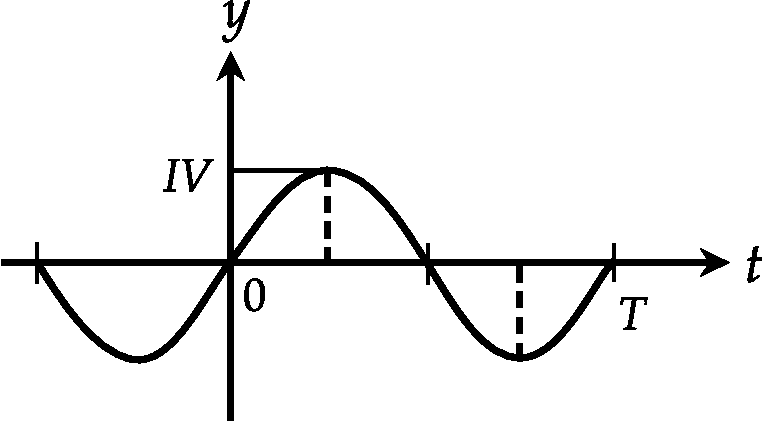
\includegraphics[height=4cm,width=8cm]{diagram-20211005(11)-crop}
		\end{figure}
		\begin{align*}
		y&=1 \sin \left(2 \pi f_{0} t\right)\\
		\text{The Fourier transform is:}\\
		F(y)&=\frac{1}{2}\left[\delta\left(f+f_{0}\right)\right]-\delta\left[f-f_{0}\right]\\
		\text{In Fourier domain }\bar{f}&=f_{0}, \bar{A}=\frac{1}{2}
		\end{align*}
		So the correct answer is \textbf{Option (B)}
	\end{answer}
	\item The Fourier transform of the derivative of the Dirac $\delta-$ function, namely $\delta^{\prime}(x)$, is proportional to
	{\exyear{NET/JRF(DEC-2013)}}
	\begin{tasks}(4)
		\task[\textbf{A.}] 0
		\task[\textbf{B.}] 1
		\task[\textbf{C.}] $\sin k$
		\task[\textbf{D.}] $i k$
	\end{tasks}
	\begin{answer}
		\begin{align*}
		\text{Fourier transform of }\delta^{\prime}(x)\\
		H(K)=\int_{-\infty}^{\infty} \delta^{\prime}(x) e^{i k x} d x&=i k e^{(k \cdot 0)}=i k
		\end{align*}
		So the correct answer is \textbf{Option (D)}
	\end{answer}
	\item The Laplace transform of $6 t^{3}+3 \sin 4 t$ is
	{\exyear{NET/JRF(JUNE-2015)}}
	\begin{tasks}(4)
		\task[\textbf{A.}] $\frac{36}{s^{4}}+\frac{12}{s^{2}+16}$
		\task[\textbf{B.}] $\frac{36}{s^{4}}+\frac{12}{s^{2}-16}$
		\task[\textbf{C.}] $\frac{18}{s^{4}}+\frac{12}{s^{2}-16}$
		\task[\textbf{D.}] $\frac{36}{s^{3}}+\frac{12}{s^{2}+16}$
	\end{tasks}
	\begin{answer}
		\begin{align*}
		L\left[6 t^{3}+3 \sin 4 t\right] &\quad \because L\left[t^{n}\right]=\frac{\sqrt{n+1}}{s^{n+1}}\\
		\because L[\sin a t]&=\frac{a}{\left(s^{2}+a^{2}\right)}\\
		L\left[6 t^{3}+3 \sin 4 t\right]&=\frac{6 \times \sqrt{4}}{s^{4}}+\frac{3 \times 4}{s^{2}+16}=\frac{36}{s^{4}}+\frac{12}{s^{2}+16}
		\end{align*}
		So the correct answer is \textbf{Option (A)}
	\end{answer}
	\item  The Fourier transform of $f(x)$ is $\tilde{f}(k)=\int_{-\infty}^{+\infty} d x e^{i k x} f(x)$.
	If $f(x)=\alpha \delta(x)+\beta \delta^{\prime}(x)+\gamma \delta^{\prime \prime}(x)$, where $\delta(x)$ is the Dirac delta-function (and prime denotes derivative), what is $\tilde{f}(k) ?$
	{\exyear{NET/JRF(DEC-2015)}}
	\begin{tasks}(2)
		\task[\textbf{A.}] $\alpha+i \beta k+i \gamma k^{2}$
		\task[\textbf{B.}] $\alpha+\beta k-\gamma k^{2}$
		\task[\textbf{C.}]  $\alpha-i \beta k-\gamma k^{2}$
		\task[\textbf{D.}] $i \alpha+\beta k-i \gamma k^{2}$
	\end{tasks}
	\begin{answer}
		\begin{align*}
		\tilde{f}(k)&=\int_{-\infty}^{\infty} d x e^{i k x}\left(\alpha \delta(x)+\beta \delta^{\prime}(x)+\gamma \delta^{\prime \prime}(x)\right)\\
		\int_{-\infty}^{\infty} \alpha \delta(x) e^{i k x} d x&=\alpha\\
		\int_{-\infty}^{\infty} \beta \delta^{\prime}(x) e^{i k x} d x&=\beta\left[\left.e^{i k x} \delta(x)\right|_{-\infty} ^{\infty}-\int_{-\infty}^{\infty} i k e^{i k x} \delta(x) d x\right]=-i \beta k\\
		\int_{-\infty}^{\infty} \gamma \delta^{\prime \prime}(x) e^{i k x} d x&=-\gamma k^{2}
		\end{align*}
		So the correct answer is \textbf{Option (C)}
	\end{answer}
	\item  What is the Fourier transform $\int d x e^{i l x} f(x)$ of
	$$
	f(x)=\delta(x)+\sum_{n=1}^{\infty} \frac{d^{n}}{d x^{n}} \delta(x)
	$$
	where $\delta(x)$ is the Dirac delta-function?
	{\exyear{NET/JRF(JUNE-2016)}}
	\begin{tasks}(4)
		\task[\textbf{A.}]  $\frac{1}{1-i k}$
		\task[\textbf{B.}] $\frac{1}{1+i k}$
		\task[\textbf{C.}] $\frac{1}{k+i}$
		\task[\textbf{D.}] $\frac{1}{k-i}$
	\end{tasks}
	\begin{answer}
		\begin{align*}
		f(x)&=\delta(x)+\sum_{n=1}^{\infty} \frac{d^{n}}{d x^{n}} \delta(x)\\&=\sum_{n=0}^{\infty} \frac{d^{n}}{d x^{n}} \delta(x)=\sum_{n=0}^{\infty} \delta^{(n)}(x)\\
		\because F[\delta(x)]&=1 \Rightarrow F\left[\delta^{(n)}(x)\right]\\&=(-i k)^{n} F[\delta(x)]=(-i k)^{n}\\
		\because f(x)&=\sum_{n=0}^{\infty} \delta^{(n)}(x)\\
		\Rightarrow F[f(x)]&=\sum_{n=0}^{\infty}(-i k)^{n}=1-i k+(i k)^{2}-(i k)^{3}+\ldots .\\&=\frac{1}{1-(-i k)}=\frac{1}{1+i k}
		\end{align*}
		So the correct answer is \textbf{Option (B)}
	\end{answer}
	\item The Laplace transform of
	$$
	f(t)=\left\{\begin{array}{cc}
	\frac{t}{T}, & 0<t<T \\
	1 & t>T
	\end{array}\right.
	$$
	is
	{\exyear{NET/JRF(DEC-2016)}}
	\begin{tasks}(4)
		\task[\textbf{A.}] $\frac{-\left(1-e^{-s T}\right)}{s^{2} T}$
		\task[\textbf{B.}] $\frac{\left(1-e^{-s T}\right)}{s^{2} T}$
		\task[\textbf{C.}] $\frac{\left(1+e^{-s T}\right)}{s^{2} T}$
		\task[\textbf{D.}] $\frac{\left(1-e^{s T}\right)}{s^{2} T}$
	\end{tasks}
	\begin{answer}
		\begin{align*}
		\intertext{we can write}
		f(t)&=\left[u_{0}(t)-u_{T}(t)\right] \frac{t}{T}+u_{T}(t)\\&=\left[1-u_{T}(t)\right] \frac{t}{T}+u_{T}(t)=\frac{t}{T}-u_{T}(t) \frac{t}{T}+u_{T}(t)
		\intertext{Hence the transform of $f(t)$ is}
		L\{f(t)\}&=L\left\{\frac{t}{T}\right\}-L\left\{u_{T}(t)\left[\frac{(t-T)+T}{T}\right]\right\}+L\left\{u_{T}(t)\right\}\\
		&=\frac{1}{s^{2} T}-\frac{e^{-s T}}{T}\left(\frac{1}{s^{2}}+\frac{T}{s}\right)+\frac{e^{-s T}}{s}=\frac{1-e^{-s T}}{s^{2} T}
		\end{align*}
		So the correct answer is \textbf{Option (B)}
	\end{answer}
	\item The Fourier transform $\int_{-\infty}^{\infty} d x f(x) e^{i k x}$ of the function $f(x)=\frac{1}{x^{2}+2}$ is
	{\exyear{NET/JRF(DEC-2016)}}
	\begin{tasks}(4)
		\task[\textbf{A.}] $\sqrt{2} \pi e^{-\sqrt{2}|| \mid}$
		\task[\textbf{B.}] $\sqrt{2} \pi e^{-\sqrt{2 k}}$
		\task[\textbf{C.}] $\frac{\pi}{\sqrt{2}} e^{-\sqrt{2 k}}$
		\task[\textbf{D.}] $\frac{\pi}{\sqrt{2}} e^{-\sqrt{2}|k|}$
	\end{tasks}
	\begin{answer}
		\begin{align*}
		\text{Fourier transform of }f(x)&=\frac{1}{x^{2}+a^{2}}, \\ a>0\text{ is }\int \frac{1}{x^{2}+a^{2}} e^{i k x} d x&=\frac{\pi}{a} e^{-a|k|}\\
		\text{Hence }\int \frac{1}{x^{2}+a^{2}} e^{i k x} d x&=\frac{\pi}{\sqrt{2}} e^{-\sqrt{2}|k|}
		\end{align*}
		So the correct answer is \textbf{Option (D)}
	\end{answer}
	\item Consider the differential equation $\frac{d y}{d t}+a y=e^{-b t}$ with the initial condition $y(0)=0$. Then the Laplace transform $Y(s)$ of the solution $y(t)$ is
	{\exyear{NET/JRF(DEC-2017)}}
	\begin{tasks}(4)
		\task[\textbf{A.}] $\frac{1}{(s+a)(s+b)}$
		\task[\textbf{B.}] $\frac{1}{b(s+a)}$
		\task[\textbf{C.}] $\frac{1}{a(s+b)}$
		\task[\textbf{D.}] $\frac{e^{-a}-e^{-b}}{b-a}$
	\end{tasks}
	\begin{answer}
		\begin{align*}
		\text{Given }\frac{d y}{d t}+a y&=e^{-b t}
		\intertext{Taking Laplace transform of both sides}
		\text{	We obtain}\\
		L\left\{\frac{d y}{d t}\right\}+a L\{y(t)\}&=L\left\{e^{-b t}\right\} \Rightarrow s Y(s)-y(0)+a Y(s)=\frac{1}{s+b}\\
		\text{Since, }	y(0)&=0,\text{ we obtain}\\
		(s+a) Y(s)&=\frac{1}{s+b} \Rightarrow Y(s)=\frac{1}{(s+a)(s+b)}
		\end{align*}
		So the correct answer is \textbf{Option (A)}
	\end{answer}
	\item  The Fourier transform $\int_{-\infty}^{\infty} d x f(x) e^{i k x}$ of the function $f(x)=e^{-|x|}$
	{\exyear{NET/JRF(JUNE-2018)}}
	\begin{tasks}(4)
		\task[\textbf{A.}] $-\frac{2}{1+k^{2}}$
		\task[\textbf{B.}] $-\frac{1}{2\left(1+k^{2}\right)}$
		\task[\textbf{C.}] $\frac{2}{1+k^{2}}$
		\task[\textbf{D.}] $\frac{2}{\left(2+k^{2}\right)}$
	\end{tasks}
	\begin{answer}
		\begin{align*}
		\int_{-\infty}^{+\infty} d x e^{-|x|} e^{i k x}&=\int_{-\infty}^{+\infty} d x e^{-|x|} \cos k x d x\text{ odd functions in }k x\text{ vanishes}\\
		\Rightarrow 2 \int_{0}^{\infty} e^{-x} \cos k x d x&=2 \frac{e^{-x}}{1+k^{2}}[-\cos k x+k \sin k x]_{0}^{\infty}\\
		\because \int e^{a x} \cos b x d x&=\frac{e^{a x}}{a^{2}+b^{2}}[a \cos b x+b \sin b x]\\
		\Rightarrow 2 \int_{0}^{\infty} e^{-x} \cos k x d x&=2 \frac{e^{0}}{1+k^{2}}=\frac{2}{1+k^{2}}
		\end{align*}
		So the correct answer is \textbf{Option (C)}
	\end{answer}
	\item The function $f(t)$ is a periodic function of period $2 \pi$. In the range $(-\pi, \pi)$, it equals $e^{-t}$. If $f(t)=\sum_{-\infty}^{\infty} c_{n} e^{\text {int }}$ denotes its Fourier series expansion, the sum $\sum_{-\infty}^{\infty}\left|c_{n}\right|^{2}$ is
	{\exyear{NET/JRF(DEC-2019)}}
	\begin{tasks}(4)
		\task[\textbf{A.}] 1
		\task[\textbf{B.}] $\frac{1}{2 \pi}$
		\task[\textbf{C.}] $\frac{1}{2 \pi} \cosh (2 \pi)$
		\task[\textbf{D.}]  $\frac{1}{2 \pi} \sinh (2 \pi)$
	\end{tasks}
	\begin{answer}
		\begin{align*}
		f(t)&=e^{-t} \quad-\pi<x<\pi\\
		f(t)&=\sum_{-\infty}^{\infty} c_{n} e^{\mathrm{int}}\\
		\sum_{-\infty}^{\infty}\left|c_{n}\right|^{2}&=\frac{1}{2 \pi} \int_{-\pi}^{\pi} e^{-2 t} d t=\left.\frac{1}{2 \pi} \cdot \frac{e^{-2 t}}{-2}\right|_{-\pi} ^{\pi}\\&=\frac{1}{2 \pi}\left[\frac{e^{-2 \pi}-e^{2 \pi}}{-2}\right]=\frac{1}{2 \pi} \sinh 2 \pi
		\end{align*}
		So the correct answer is \textbf{Option (D)}
	\end{answer}
\end{enumerate}
\colorlet{ocre1}{ocre!70!}
\colorlet{ocrel}{ocre!30!}
\setlength\arrayrulewidth{1pt}
\begin{table}[H]
	\centering
	\arrayrulecolor{ocre}
	\begin{tabular}{|p{1.5cm}|p{1.5cm}||p{1.5cm}|p{1.5cm}|}
		\hline
		\multicolumn{4}{|c|}{\textbf{Answer key}}\\\hline\hline
		\rowcolor{ocrel}Q.No.&Answer&Q.No.&Answer\\\hline
		1&\textbf{B} &2&\textbf{B}\\\hline 
		3&\textbf{D} &4&\textbf{A} \\\hline
		5&\textbf{C} &6&\textbf{B} \\\hline
		7&\textbf{B}&8&\textbf{D}\\\hline
		9&\textbf{A}&10&\textbf{C}\\\hline
		11&\textbf{D} &&\textbf{}\\\hline
		
	\end{tabular}
\end{table}

\newpage
\begin{abox}
	Practise Set-2
\end{abox}
\begin{enumerate}[label=\color{ocre}\textbf{\arabic*.}]
	\item If $f(x)=\left\{\begin{array}{ll}0 & \text { for } x<3, \\ x-3 & \text { for } x \geq 3\end{array}\right.$ then the Laplace transform of $f(x)$ is
	{\exyear{GATE 2010}}
	\begin{tasks}(4)
		\task[\textbf{A.}] $s^{-2} e^{3 s}$
		\task[\textbf{B.}] $s^{2} e^{3 s}$
		\task[\textbf{C.}] $s^{-2}$
		\task[\textbf{D.}] $s^{-2} e^{-3 s}$
	\end{tasks}
	\begin{answer}
		\begin{align*}
		L\{f(x)\}&=\int_{0}^{\infty} e^{-s x} f(x) d x\\&=\int_{0}^{3} e^{-s x} f(x) d x+\int_{3}^{\infty} e^{-s x} f(x) d x\\&=\int_{3}^{\infty}(x-3) e^{-s x} d x\\
		L\{f(x)\}&=\left.(x-3) \frac{e^{-s x}}{-s}\right|_{3} ^{\infty}-\int_{3}^{\infty} 1 \cdot\left(\frac{e^{-s x}}{-s}\right) d x\\&=0+\frac{1}{s} \int_{3}^{\infty} e^{-s x} d x\\&=\frac{1}{s}\left[\frac{e^{-s x}}{-s}\right]_{3}^{\infty}=s^{-2} e^{-3 s}
		\end{align*}
		So the correct answer is \textbf{Option (D)}
	\end{answer}
	\item The coefficient of $e^{i k x}$ in the Fourier expansion of $u(x)=A \sin ^{2}(\alpha x)$ for $k=-2 \alpha$ is
	{\exyear{GATE 2017}}
	\begin{tasks}(4)
		\task[\textbf{A.}] $\frac{A}{4}$
		\task[\textbf{B.}] $\frac{-A}{4}$
		\task[\textbf{C.}] $\frac{A}{2}$
		\task[\textbf{D.}] $\frac{-A}{2}$
	\end{tasks}
	\begin{answer}
		\begin{align*}
		\text{	Since, }\sin (\alpha x)&=\frac{e^{i \alpha x}-e^{-i \alpha x}}{2 i} \Rightarrow \sin ^{2}(\alpha x)\\&=\frac{e^{i 2 \alpha x}-2+e^{-2 i \alpha x}}{(-4)}\\
		\text{Since, }2 \alpha&=-k,\text{ hence }\sin ^{2}(\alpha x)\\&=\frac{e^{-i k x}-2+e^{i k x}}{(-4)}\\
		\text{Hence, }c_{k}&=\frac{A}{2 \pi} \int_{-\pi}^{\pi} \sin ^{2}(\alpha x) d x\\&=-\frac{A}{8 \pi}\left[\int_{-\pi}^{\pi} e^{-i k x} e^{-i k x} d x-2 \int_{-\pi}^{\pi} e^{-i k x} d x+\int_{-\pi}^{\pi} e^{-i k x} e^{i k x} d x\right]\\
		&=-\frac{A}{8 \pi}\left[\int_{-\pi}^{\pi} e^{-2 i k x} d x-2 \int_{-\pi}^{\pi} e^{-i k x} d x+\int_{-\pi}^{\pi} d x\right]
		\intertext{The first two integrals are zero and the third integral has the value $2 \pi$.
			Thus,}
		c_{k}&=-\frac{A}{8 \pi}(2 \pi)=-\frac{A}{4}
		\end{align*}
		So the correct answer is \textbf{Option (B)}
	\end{answer}
	\item Given the fundamental constants $\hbar$ (Planck's constant), $G$ (universal gravitation constant) and $c$ (speed of light), which of the following has dimension of length?
	{\exyear{JEST 2014}}
	\begin{tasks}(2)
		\task[\textbf{A.}]$\sqrt{\frac{\hbar G}{c^{3}}}$
		\task[\textbf{B.}] $\sqrt{\frac{\hbar G}{c^{5}}}$
		\task[\textbf{C.}]$\frac{\hbar G}{c^{3}}$
		\task[\textbf{D.}] $\sqrt{\frac{\hbar c}{8 \pi G}}$
	\end{tasks}
	\begin{answer}
		\begin{align*}
		\left[\frac{\left[M L^{2} T^{-1}\right]\left[M^{-1} L^{3} T^{-2}\right]}{L^{3} T^{-3}}\right]^{\frac{1}{2}}&=\left[L^{2}\right]^{\frac{1}{2}}=L\\
		\hbar=\left[M L^{2} T^{-1}\right], G=\frac{g r^{2}}{m}&=\left[M^{-1} L^{3} T^{-2}\right]
		\end{align*}
		So the correct answer is \textbf{Option (A)}
	\end{answer}
	\item The Fourier transform of the function $\frac{1}{x^{4}+3 x^{2}+2}$ up to proportionality constant is
	{\exyear{JEST 2017}}
	\begin{tasks}(2)
		\task[\textbf{A.}]$\sqrt{2} \exp \left(-k^{2}\right)-\exp \left(-2 k^{2}\right)$
		\task[\textbf{B.}]$\sqrt{2} \exp (-|k|)-\exp (-\sqrt{2}|k|)$
		\task[\textbf{C.}]$\sqrt{2} \exp (-\sqrt{|k|})-\exp (-\sqrt{2|k|})$
		\task[\textbf{D.}]  $\sqrt{2} \exp \left(-\sqrt{2} k^{2}\right)-\exp \left(-2 k^{2}\right)$
	\end{tasks}
	\begin{answer}
		\begin{align*}
		f(x)&=\frac{1}{\left(x^{4}+3 x^{2}+2\right)}=\frac{1}{\left(x^{2}+1\right)}-\frac{1}{\left[x^{2}+(\sqrt{2})^{2}\right]}
		\intertext{Now, Fourier transform of $f(x)$ is,}
		F(p)&=A \int_{-\infty}^{\infty} f(x) e^{-1 k x} d x\\
		&=A \int_{-\infty}^{\infty}\left[\frac{1}{\left(x^{2}+1\right)}-\frac{1}{x^{2}+(\sqrt{2})^{2}}\right] e^{-i k x} d x=A\left[\int_{-\infty}^{\infty} \frac{1}{\left(x^{2}+1\right)} \times e^{-i k x} d x-\int_{-\infty}^{\infty} \frac{e^{-i k x}}{x^{2}+(\sqrt{2})^{2}} d x\right]\\
		\because &\int_{-\infty}^{\infty} \frac{1}{\left(x^{2}+a^{2}\right)} e^{-i k x} d x=\sqrt{\frac{\pi}{2}} \frac{e^{-a|k|}}{a}\\
		F(k)&=A\left[\sqrt{\frac{\pi}{2}} \frac{e^{-|k|}}{1}-\sqrt{\frac{\pi}{2}} \frac{e^{-\sqrt{2} \mid k}}{\sqrt{2}}\right]=\frac{A \sqrt{\pi}}{2}[\sqrt{2} \exp (-|k|)-\exp (-\sqrt{2}|k|)]\\
		\end{align*}
		So the correct answer is \textbf{Option (B)}
	\end{answer}
	\item The function $f(x)=\cosh x$ which exists in the range $-\pi \leq x \leq \pi$ is periodically repeated between $x=(2 m-1) \pi$ and $(2 m+1) \pi$, where $m=-\infty$ to $\infty$. Using Fourier series, indicate the correct relation at $x=0$
	{\exyear{JEST 2017}}
	\begin{tasks}(2)
		\task[\textbf{A.}] $\sum_{n=-\infty}^{\infty} \frac{(-1)^{n}}{1-n^{2}}=\frac{1}{2}\left(\frac{\pi}{\cosh \pi}-1\right)$
		\task[\textbf{B.}]$\sum_{n=-\infty}^{\infty} \frac{(-1)^{n}}{1-n^{2}}=2 \frac{\pi}{\cosh \pi}$
		\task[\textbf{C.}]$\sum_{n=-\infty}^{\infty} \frac{(-1)^{-n}}{1+n^{2}}=2 \frac{\pi}{\sinh \pi}$
		\task[\textbf{D.}] $\sum_{n=1}^{\infty} \frac{(-1)^{n}}{1+n^{2}}=\frac{1}{2}\left(\frac{\pi}{\sinh \pi}-1\right)$
	\end{tasks}
	\begin{answer}
		\begin{align*}
		f(x)&=\cosh x, \quad-\pi \leq x \leq \pi\\
		\text{Here, }a_{0}&=\frac{1}{2 \pi} \int_{-\pi}^{\pi} \cosh x d x=\frac{1}{2 \pi}[\sinh x]_{-\pi}^{\pi}=\frac{\sinh \pi}{\pi}\\
		b_{n}&=0,\text{ due to even function}\\
		\text{	and }a_{n}&=\frac{1}{2 \pi} \int_{-\pi}^{\pi}\left(e^{x}+e^{-x}\right) \cos n x d x\qquad
		\left[\because \cosh x=\frac{1}{2}\left(e^{x}+e^{-x}\right)\right]\\
		a_{n}&=\frac{1}{2 \pi}\left[\frac{e^{x}}{\left(1+n^{2}\right)}(\cos n x+n \sin n x)+\frac{e^{-x}}{1+n^{2}}(-\cos n x+n \sin n x)\right]_{-\pi}^{\pi}\\
		&=\frac{1}{2 \pi}\left[\frac{e^{\pi}(-1)^{n}}{\left(1+n^{2}\right)}-\frac{e^{-\pi}(-1)^{n}}{\left(1+n^{2}\right)}-\frac{e^{-\pi}(-1)^{n}}{\left(1+n^{2}\right)}+\frac{e^{\pi}(-1)^{n}}{\left(1+n^{2}\right)}\right]\\&=\frac{2(-1)^{n} \cdot 2 \sinh \pi}{2 \pi\left(1+n^{2}\right)}=\frac{2(-1)^{n} \sinh \pi}{\pi\left(1+n^{2}\right)}\\
		\text{	Hence, }f(x)&=a_{0}+\sum_{n=1}^{\infty}\left(a_{n} \cos n x+b_{n} \sin n x\right) \Rightarrow \cosh x=\frac{\sinh \pi}{\pi}+\sum_{n=1}^{\infty} \frac{2(-1)^{n} \sinh \pi}{\pi\left(1+n^{2}\right)} \cos n x\\
		\text{At }x&=0,\\
		\sum_{n=1}^{\infty} \frac{2(-1)^{n} \sinh \pi}{\pi\left(1+n^{2}\right)}&=\left(1-\frac{\sinh \pi}{\pi}\right) \Rightarrow \sum_{n=1}^{\infty} \frac{(-1)^{n}}{\left(1+n^{2}\right)}=\frac{1}{2}\left[\frac{\pi}{\sinh \pi}-1\right]
		\end{align*}
		So the correct answer is \textbf{Option (D)}
	\end{answer}
	\item The Laplace transform of $\frac{(\sin (a t)-a t \cos (a t))}{\left(2 a^{3}\right)}$ is
	{\exyear{JEST 2018}}
	\begin{tasks}(2)
		\task[\textbf{A.}]$\frac{2 a s}{\left(s^{2}+a^{2}\right)^{2}}$
		\task[\textbf{B.}]$\frac{s^{2}-a^{2}}{\left(s^{2}+a^{2}\right)^{2}}$
		\task[\textbf{C.}]$\frac{1}{(s+a)^{2}}$
		\task[\textbf{D.}] $\frac{1}{\left(s^{2}+a^{2}\right)^{2}}$
	\end{tasks}
	\begin{answer}
		\begin{align*}
		L\left\{\frac{\sin a t-a t \cos a t}{2 a^{3}}\right\}=\frac{1}{\left(s^{2}+a^{2}\right)^{2}}
		\end{align*}
		So the correct answer is \textbf{Option (D)}
	\end{answer}
\end{enumerate}
\colorlet{ocre1}{ocre!70!}
\colorlet{ocrel}{ocre!30!}
\setlength\arrayrulewidth{1pt}
\begin{table}[H]
	\centering
	\arrayrulecolor{ocre}
	\begin{tabular}{|p{1.5cm}|p{1.5cm}||p{1.5cm}|p{1.5cm}|}
		\hline
		\multicolumn{4}{|c|}{\textbf{Answer key}}\\\hline\hline
		\rowcolor{ocrel}Q.No.&Answer&Q.No.&Answer\\\hline
		1&\textbf{D} &2&\textbf{B}\\\hline 
		3&\textbf{A} &4&\textbf{B} \\\hline
		5&\textbf{D} &6&\textbf{D} \\\hline
		
	\end{tabular}
\end{table}
\chapter{Assignment}
\section{MCQ}
\begin{enumerate}
	\item One of the possible solutions of the differential equation
	$y \sqrt{\left(1+x^{2}\right)} d y+x \sqrt{\left(1+y^{2}\right)} d x=0$ (where $c$ is some constant) is
	 \begin{tasks}(2)
		\task[\textbf{a.}]$\left(\sqrt{1+y^{2}}\right)\left(\sqrt{1+x^{2}}\right)=c$
		\task[\textbf{b.}]$\frac{\sqrt{1+y^{2}}}{\sqrt{1+x^{2}}}=c$
		\task[\textbf{c.}]$\sqrt{1+y^{2}}+\sqrt{1+x^{2}}=c$
		\task[\textbf{d.}]  $\sqrt{1+y^{2}}-\sqrt{1+x^{2}}=c$
	\end{tasks}
	\item The solution of the differential equation $x \frac{d y}{d x}+\cot y=0$, subject to the initial condition $y=\frac{\pi}{4}$ at $x=\sqrt{2}$ is
	 \begin{tasks}(2)
		\task[\textbf{a.}]$x=2 \cos y$
		\task[\textbf{b.}]$x=2 \sec y$
		\task[\textbf{c.}]$x=2 \sin y$
		\task[\textbf{d.}]  $x=2 \operatorname{cosecy}$
	\end{tasks}
	\item The solutions to the differential equation $\frac{d y}{d x}=-\frac{x}{y+1}$ are a family of
	 \begin{tasks}(2)
		\task[\textbf{a.}]Circles with different radii
		\task[\textbf{b.}]Circles with different centres
		\task[\textbf{c.}]Straight lines with different slopes
		\task[\textbf{d.}] Straight lines with different intercepts on the $y$-axis
	\end{tasks}
	\item The solution of the differential equation $x y \frac{d y}{d x}=3 y^{2}+x^{2}$ with the initial condition $y=2$ when $x=1$ is
	 \begin{tasks}(2)
		\task[\textbf{a.}]$2 y^{2}+x^{2}=9 x^{6}$
		\task[\textbf{b.}] $y^{2}+2 x^{2}=9 x^{6}$
		\task[\textbf{c.}] $2 y^{2}+x^{2}=8 x^{6}$
		\task[\textbf{d.}] $y^{2}+2 x^{2}=8 x^{6}$
	\end{tasks}
	\item The solution of the differential equation
	$(x+2 y)(d x-d y)=d x+d y$ (where $a$ is some constant) is
	 \begin{tasks}(2)
		\task[\textbf{a.}]$3 x+3 y+a=2 \log (3 x+6 y-1)$
		\task[\textbf{b.}] $3 x-3 y+a=2 \log (3 x+6 y-1)$
		\task[\textbf{c.}]$3 x-3 y+a=2 \log (3 x-6 y-1)$
		\task[\textbf{d.}] $3 x+3 y+a=2 \log (3 x-6 y-1)$
	\end{tasks}
	\item For the differential equation $\frac{d y}{d x}+3 y=e^{2 x}$, the possible solution is:
	 \begin{tasks}(2)
		\task[\textbf{a.}]$y=c_{1} e^{2 x}+c_{2} e^{3 x}$
		\task[\textbf{b.}]$y=c_{1} e^{-2 x}+c_{2} e^{3 x}$
		\task[\textbf{c.}]$y=c_{1} e^{2 x}+c_{2} e^{-3 x}$
		\task[\textbf{d.}] $y=c_{1} e^{-2 x}+c_{2} e^{-3 x}$
	\end{tasks}
	\item The solution of the differential equation for $y: x \frac{d y}{d x}+y=x^{4}$, subject to the initial condition $y=1$ at $x=1$ is
	 \begin{tasks}(2)
		\task[\textbf{a.}]$y=5 x^{4}-4$
		\task[\textbf{b.}]$y=\frac{x^{4}}{5}+\frac{4 x}{5}$
		\task[\textbf{c.}] $y=\frac{x^{4}}{5}+\frac{1}{5 x}$
		\task[\textbf{d.}] $y=\frac{x^{4}}{5}+\frac{4}{5 x}$
	\end{tasks}
	\item Which one of the following curves gives the solution of the differential equation $K_{1} \frac{d x}{d t}+K_{2} x=K_{3}$, where $K_{1}, K_{2}$ and $K_{3}$ are positive constants with initial conditions $x=0$ at $t=0$ ?
	 \begin{tasks}(2)
		\task[\textbf{a.}]
		\begin{figure}[H]
			\centering
			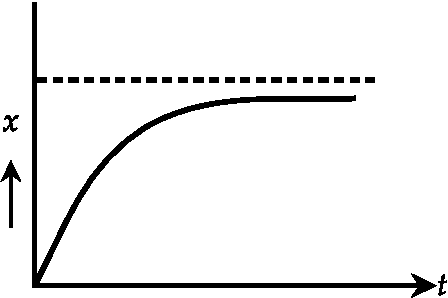
\includegraphics[height=2.5cm,width=4cm]{DE -assignment-04}
		\end{figure}
		\task[\textbf{b.}]	
		\begin{figure}[H]
			\centering
			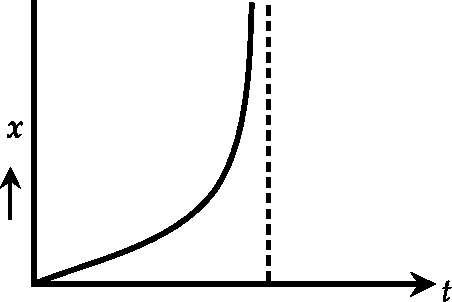
\includegraphics[height=2.5cm,width=4cm]{DE -assignment-01}
		\end{figure}
		\task[\textbf{c.}]
			\begin{figure}[H]
			\centering
			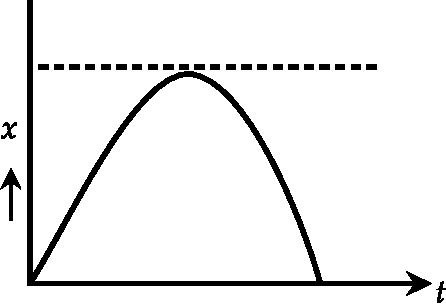
\includegraphics[height=2.5cm,width=4cm]{DE -assignment-02}
		\end{figure}
		\task[\textbf{d.}]
			\begin{figure}[H]
			\centering
			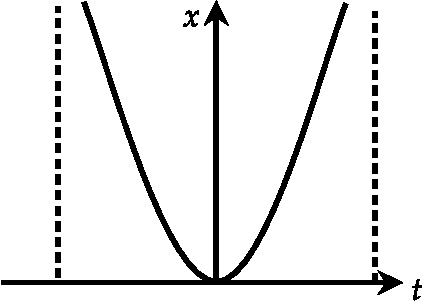
\includegraphics[height=2.5cm,width=4cm]{DE -assignment-03}
		\end{figure}
	\end{tasks}
	\item The solution of the differential equation $t \frac{d y}{d t}+y \log y=t y e^{t}$
	 \begin{tasks}(2)
		\task[\textbf{a.}]$\log y=(t+1) e^{t}+c$
		\task[\textbf{b.}]$\log y=(t-1) e^{t}+c$
		\task[\textbf{c.}]$t \log y=(t+1) e^{t}+c$
		\task[\textbf{d.}] $t \log y=(t-1) e^{t}+c$
	\end{tasks}
	\item The solution of the differential equation
	$\left(1+y^{2}\right) d x=\left(\tan ^{-1} y-x\right) d y$ (where $c$ is some constant) is
	 \begin{tasks}(2)
		\task[\textbf{a.}] $x=\left(\tan ^{-1} y+2\right)+c e^{-\tan ^{-1} y}$
		\task[\textbf{b.}] $x=\left(\tan ^{-1} y-2\right)+c e^{-\tan ^{-1} y}$
		\task[\textbf{c.}] $x=\left(\tan ^{-1} y+1\right)+c e^{-\tan ^{-1} y}$
		\task[\textbf{d.}]  $x=\left(\tan ^{-1} y-1\right)+c e^{-\tan ^{-1}y}$
	\end{tasks}
	\item The solution of the differential equation
	$y \log y \frac{d x}{d y}+x-\log y=0$ (where $c$ is some constant) is
	 \begin{tasks}(2)
		\task[\textbf{a.}]$x \log y=\frac{1}{2}(\log y)^{2}+c$
		\task[\textbf{b.}] $x \log y=2(\log y)^{2}+c$
		\task[\textbf{c.}]$x \log y=\frac{1}{2}(\log y)^{3}+c$
		\task[\textbf{d.}]  $y \log x=\frac{1}{2}(\log y)^{2}+c$
	\end{tasks}
	\item The solution of the differential equation
	$\left(e^{y}+2\right) \sin x d x-e^{y} \cos x d y=0$ (where $c$ is some constant) is
	 \begin{tasks}(2)
		\task[\textbf{a.}]$\left(e^{y}+2\right) \sin x=c$
		\task[\textbf{b.}] $\left(e^{y}+2\right) \cos x=c$
		\task[\textbf{c.}] $\left(e^{y}+2\right) \operatorname{cosec} x=c$
		\task[\textbf{d.}] $\left(e^{y}+2\right) \sec x=c$
	\end{tasks}
	\item For the differential equation $\left(y^{4}+2 y\right) d x+\left(x y^{3}+2 y^{4}-4 x\right) d y=0$ one of the possible solution (where $C$ is some constant) is:
	 \begin{tasks}(2)
		\task[\textbf{a.}]$x+\frac{2}{y^{2}}+y^{2}=c$
		\task[\textbf{b.}] $x\left(y+\frac{2}{y^{2}}\right)=c$
		\task[\textbf{c.}]$x\left(y+\frac{2}{y^{2}}\right)+y^{2}=c$
		\task[\textbf{d.}] $x\left(1+\frac{2}{y^{2}}\right)+x^{2}=c$
	\end{tasks}
	\item The solution of the differential equation for $y(t): \frac{d^{2} y}{d t^{2}}-\frac{3 d y}{d t}+2 y=e^{3 t}$ is
	 \begin{tasks}(2)
		\task[\textbf{a.}] $c_{1} e^{t}+c_{2} e^{2 t}+\frac{1}{2} e^{3 t}$
		\task[\textbf{b.}]$c_{1} e^{-t}+c_{2} e^{2 t}+\frac{1}{2} e^{3 t}$
		\task[\textbf{c.}]$c_{1} e^{t}+c_{2} e^{2 t}+e^{3 t}$
		\task[\textbf{d.}] $c_{1} e^{-t}+c_{2} e^{-2 t}+e^{3 t}$
	\end{tasks}
	\item The solution of the differential equation for $\frac{d^{2} y}{d x^{2}}+2 \frac{d y}{d x}+101 y=10.4 e^{x}$, subject to the initial conditions $y(0)=1.1$ and $\left.\frac{d y}{d x}\right|_{x=0}=-0.9$, is
	 \begin{tasks}(2)
		\task[\textbf{a.}]$e^{-x} \cos 10 x+0.1 e^{x}$
		\task[\textbf{b.}]$e^{-x} \sin 10 x+0.1 e^{x}$
		\task[\textbf{c.}]$e^{x} \cos 10 x+0.1 e^{-x}$
		\task[\textbf{d.}] $e^{x} \sin 10 x+0.1 e^{-x}$
	\end{tasks}
	\item The solution of the differential equation $\frac{d^{2} y}{d t^{2}}+4 y=\cos 2 t$ is:
	 \begin{tasks}(2)
		\task[\textbf{a.}] $A \cos 2 t+B \sin 2 t$
		\task[\textbf{b.}] $\frac{t \sin 2 t}{4}$
		\task[\textbf{c.}]$A \cos 2 t+B \sin 2 t+\frac{t \sin 2 t}{4}$
		\task[\textbf{d.}] $A \cos 2 t+B \sin 2 t+\frac{t^{2} \sin 2 t}{4}$
	\end{tasks}
	\item The solution of the differential equation for $y(t): \frac{d^{2} y}{d t^{2}}-y=2 \cosh (t)$, subject to the initial conditions $y(0)=0$ and $\left.\frac{d y}{d t}\right|_{t=0}=0$, is
	 \begin{tasks}(2)
		\task[\textbf{a.}]$\frac{1}{2} \cosh (t)+t \sin h(t)$
		\task[\textbf{b.}]$-\sin h(t)+t \cosh (t)$
		\task[\textbf{c.}] $t \cosh (t)$
		\task[\textbf{d.}] $t \sin h(t)$
	\end{tasks}
	\item The solution of the differential equation for $y(t): \frac{d^{2} y}{d t^{2}}-y=2 \sinh (t)$, subject to the initial conditions $y(0)=0$ and $\left.\frac{d y}{d t}\right|_{t=0}=0$, is
	 \begin{tasks}(2)
		\task[\textbf{a.}] $\frac{1}{2} \cosh (t)+t \sin h(t)$
		\task[\textbf{b.}]$-\sin h(t)+t \cosh (t)$
		\task[\textbf{c.}]$t \cosh (t)$
		\task[\textbf{d.}] $t \sin h(t)$
	\end{tasks}
\end{enumerate}
\section{NAT}
\begin{enumerate}
	\item The solution of the differential equation $\frac{d x}{d t}=x^{2}$ with the initial condition $x(0)=1$ will blow up as $t$ tends to..........
	\item The value of $\lambda \ldots .$ for which the differential equation $\left(x y^{2}+\lambda x^{2} y\right) d x+(x+y) x^{2} d y=0$ is exact
	\item The particular integral of the differential equation $\left(D^{2}+D+1\right) y=\cos 2 x$ is $\frac{1}{\alpha}(2 \sin 2 x-3 \cos 2 x) .$ Then the value of $\alpha$ is.....
	\item The particular integral of the differential equation $\frac{d^{2} y}{d x^{2}}+2 \frac{d y}{d x}+2 y=\sin x$ is $\frac{1}{5}(\sin x-\alpha \cos x) .$ Then the value of $\alpha$ is........
	\item The particular integral of the differential equation $\left(D^{2}-5 D+6\right) y=e^{t} \cos 2 t$ is $-\frac{e^{t}}{20}(\alpha \sin 2 t+\cos 2 t)$. Then the value of $\alpha$ is........
	\item The particular integral of the differential equation $\left(D^{2}-4 D+4\right) y=x^{3} e^{2 x}$ is $e^{2 x} \frac{x^{\alpha}}{20}$. Then the value of $\alpha$ is........
	\item The particular integral of the differential equation $\left(D^{2}+5 D+4\right) y=3-2 x$ is $\frac{1}{8}[\alpha-4 x]$.
	Then the value of $\alpha$ is........
	\item The maximum value of the solution $y(t) \ldots \ldots \ldots . .$ of the differential equation for $y(t)+\ddot{y}(t)=0$, subject to the initial conditions $\dot{y}(0)=1$ and $y(0)=1$ for $t \geq 0$, is
	\item If the characteristic equation $\frac{d^{2} y}{d x^{2}}+2 \alpha \frac{d x}{d t}+y=0$ has two equal roots, then the value of $\alpha \ldots \ldots \ldots$ is
	\item Consider the differential equation $\frac{d^{2} x}{d t^{2}}+3 \frac{d x}{d t}+2 x=0 .$ Given $x(0)=20$ and $x(1)=\frac{10}{e}$, where $e=2.718$, the value of $x(2)$ is
\end{enumerate}

\chapter{Assignment- Differential Equations}
\section{MCQ}
\begin{enumerate}
	\item $\left. \right. $
	\begin{answer}
		\begin{align*}
			\int \frac{y}{\sqrt{1+y^{2}}} d y+\int \frac{x}{\sqrt{1+x^{2}}} d x=c \Rightarrow \sqrt{1+y^{2}}+\sqrt{1+x^{2}}=c
		\end{align*}
		So the correct answer is \textbf{Option (c)}
	\end{answer}
	\item $\left. \right. $
	\begin{answer}
		\begin{align*}
		x d y&=-\cot y d x \Rightarrow \tan y d y=-\frac{d x}{x}\\
		\Rightarrow \int \tan y d y&=-\int \frac{d x}{x}+\log A \Rightarrow \log \sec y=-\log x+\log A \Rightarrow \log \sec y=\log \frac{A}{x}\\
		\Rightarrow x&=A \cos y \Rightarrow \sqrt{2}=A \cos \frac{\pi}{4} \Rightarrow A=2 \Rightarrow x=2 \cos y
		\end{align*}
		So the correct answer is \textbf{Option (a)}
	\end{answer}
	\item $\left. \right. $
	\begin{answer}
		\begin{align*}
		\frac{d y}{d x}&=-\frac{x}{y+1} \Rightarrow x d x+y d y+d y=0 \Rightarrow \frac{x^{2}}{2}+\frac{y^{2}}{2}+y=C_{1} \Rightarrow x^{2}+y^{2}+2 y=2 C_{1}\\
		\Rightarrow(x-0)^{2}+(y+1)^{2}&=2 C_{1}+1=C
		\intertext{which is family of circles with different radii.}
		\end{align*}
		So the correct answer is \textbf{Option (a)}
	\end{answer}
	\item $\left. \right. $
\begin{answer}
	\begin{align*}
	x y \frac{d y}{d x}&=3 y^{2}+x^{2} \Rightarrow \frac{d y}{d x}=\frac{3 y^{2}+x^{2}}{x y}\text{ which is a homogeneous equation.}\\
	\text{Put }y&=v x \Rightarrow \frac{d y}{d x}=v+x \frac{d v}{d x} \Rightarrow v+x \frac{d v}{d x}=\frac{3 v^{2} x^{2}+x^{2}}{v x^{2}}=\frac{3 v^{2}+1}{v}\\
	\Rightarrow x \frac{d v}{d x}&=\frac{3 v^{2}+1}{v}-v=\frac{2 v^{2}+1}{v} \Rightarrow \frac{v}{2 v^{2}+1} d v=\frac{d x}{x}\\
	\Rightarrow \frac{1}{4} \ln \left(2 v^{2}+1\right)&=\ln x+\ln c^{\prime} \Rightarrow \ln \left(2 v^{2}+1\right)=\ln x^{4}+\ln c \Rightarrow\left(2 v^{2}+1\right)=c x^{4}\\
	\Rightarrow\left(2 \frac{y^{2}}{x^{2}}+1\right)&=c x^{4}\\
	y=2\text{ when }x&=1 \Rightarrow\left(2 \frac{4}{1}+1\right)=c .1 \Rightarrow c=9 \Rightarrow 2 y^{2}+x^{2}=9 x^{6}
	\end{align*}
		So the correct answer is \textbf{Option (a)}
\end{answer}
	\item $\left. \right. $
\begin{answer}
	\begin{align*}
	\frac{d y}{d x}=\frac{x+2 y-1}{x+2 y+1}\text{. Let }x+2 y&=z \Rightarrow 1+2 \frac{d y}{d x}=\frac{d z}{d x} \Rightarrow \frac{d z}{d x}=\frac{3 z-1}{z+1}\\
	\Rightarrow \int\left(\frac{1}{3}+\frac{1}{4}-\frac{1}{3 z-1}\right) d z&=\int d x+c \Rightarrow \frac{z}{3}+\frac{4}{9} \log (3 z-1)=x+c\\
	\Rightarrow 3 x-3 y+a&=2 \log (3 x+6 y-1)
	\end{align*}
		So the correct answer is \textbf{Option (b)}
\end{answer}
	\item $\left. \right. $
\begin{answer}
	\begin{align*}
	\text{I.F. }=e^{\int 3 d x}&=e^{3 x} \Rightarrow y \times e^{3 x}=\int e^{2 x} \times e^{3 x} d x+c \Rightarrow y \times e^{3 x}=\frac{e^{5 x}}{5}+c \Rightarrow y=c_{1} e^{2 x}+c_{2} e^{-3 x}
	\end{align*}
		So the correct answer is \textbf{Option (c)}
\end{answer}
\item $\left. \right. $
\begin{answer}
	\begin{align*}
	\frac{d y}{d x}+\frac{1}{x} y&=x^{3} \Rightarrow \mathrm{I} . F .=e^{\int \frac{1}{x} d x}=e^{\ln x}=x\\
	\Rightarrow y \times x&=\int x^{3} \times x d x+c \Rightarrow y \times x=\frac{x^{5}}{5}+c \Rightarrow y=\frac{x^{4}}{5}+\frac{c}{x}\\
\text{	Since }y&=1\text{ at }x=1 \Rightarrow 1=\frac{1}{5}+\frac{c}{1} \Rightarrow c=\frac{4}{5} \Rightarrow y=\frac{x^{4}}{5}+\frac{4}{5 x}
	\end{align*}
		So the correct answer is \textbf{Option (d)}
\end{answer}
	\item $\left. \right. $
\begin{answer}
	\begin{align*}
	\frac{d x}{d t}+\frac{K_{2}}{K_{1}} x&=\frac{K_{3}}{K_{1}} \Rightarrow \frac{d x}{d t}+A x=B \Rightarrow I . F .=e^{\int A d t}=e^{A t} \Rightarrow x \times e^{A t}=\int\left(B \times e^{A t}\right) d t+c\\
	\Rightarrow x \times e^{A t}&=B \times \frac{e^{A t}}{A}+c \Rightarrow x=c_{1}+c e^{-A t}\\
	\text{Since }x&=0\text{ at }t=0 \Rightarrow c_{1}+c=0 \Rightarrow c_{1}=-c \Rightarrow x=c\left(1-e^{-A t}\right)
	\end{align*}
		So the correct answer is \textbf{Option (a)}
\end{answer}
	\item $\left. \right. $
\begin{answer}
	\begin{align*}
	\text{Divide by }y t \Rightarrow \frac{1}{y} \frac{d y}{d t}+\frac{1}{t} \log y&=e^{t}\text{, put }\log y=z \Rightarrow \frac{1}{y} \frac{d y}{d t}=\frac{d z}{d t}\\
	\Rightarrow \frac{d z}{d t}+\frac{1}{t} \cdot z&=e^{t} \Rightarrow I \cdot F=e^{\int_{t}^{1} d t}=e^{\log t}=t\\
	\Rightarrow z t&=\int t e^{t} d t+c \Rightarrow t \log y=t e^{t}-e^{t}+c
	\end{align*}
		So the correct answer is \textbf{Option (d)}
\end{answer}
	\item $\left. \right. $
\begin{answer}
	\begin{align*}
	\left(1+y^{2}\right) d x&=\left(\tan ^{-1} y-x\right) d y \Rightarrow \frac{d x}{d y}=\frac{\tan ^{-1} y-x}{1+y^{2}}\\
	\Rightarrow \frac{d x}{d y}+\frac{x}{1+y^{2}}&=\frac{\tan ^{-1} y}{1+y^{2}}.\text{ This is a linear differential equation.}\\
	I . F .&=e^{\int \frac{1}{1+y^{2}} d y}=e^{\tan ^{-1} y}\\
	\text{	Its solution is }x . e^{\tan ^{-1} y}&=\int e^{\tan ^{-1} y} \frac{\tan ^{-1} y}{1+y^{2}} d y+c\\
	\text{Put }\tan ^{-1} y&=t\text{ on R.H.S. so that }\frac{1}{1+y^{2}} d y=d t\\
	x . e^{\tan ^{-1} y}&=\int e^{t} t d t+C=t . e^{t}-e^{t}+C=e^{\tan ^{-1} y}\left(\tan ^{-1} y-1\right)+C\\
	\Rightarrow x&=\left(\tan ^{-1} y-1\right)+c e^{-\tan ^{-1} y}
	\end{align*}
		So the correct answer is \textbf{Option (d)}
\end{answer}
	\item $\left. \right. $
\begin{answer}
	\begin{align*}
	y \log y \frac{d x}{d y}+x-\log y&=0 \Rightarrow \frac{d x}{d y}+\frac{x}{y \log y}=\frac{1}{y}\\
	I . F .&=e^{\int \frac{1}{y \log y} d y}=e^{\log (\log y)}=\log y\\
	\text{Its solution is }x \cdot \log y&=\int \frac{1}{y}(\log y) d y+c \Rightarrow x \cdot \log y=\frac{1}{2}(\log y)^{2}+c
	\end{align*}
		So the correct answer is \textbf{Option (a)}
\end{answer}
\item $\left. \right. $
\begin{answer}
	\begin{align*}
	M&=\left(e^{y}+2\right) \sin x, N=-e^{y} \cos x \Rightarrow \frac{\partial M}{\partial y}=e^{y} \sin x, \frac{\partial N}{\partial x}=e^{y} \sin x\\
	\Rightarrow \frac{\partial M}{\partial y}&=\frac{\partial N}{\partial x} \Rightarrow \int\left(e^{y}+2\right) \sin x d x+0=c^{\prime} \Rightarrow\left(e^{y}+2\right) \cos x=-c^{\prime}=c
	\end{align*}
\end{answer}
\item $\left. \right. $
\begin{answer}
	\begin{align*}
	M&=\left(y^{4}+2 y\right), N=\left(x y^{3}+2 y^{4}-4 x\right)\\
	\Rightarrow \frac{\partial M}{\partial y}&=4 y^{3}+2, \frac{\partial N}{\partial x}=y^{3}-4 \Rightarrow \frac{\frac{\partial N}{\partial x}-\frac{\partial M}{\partial y}}{M}=-\frac{3}{y}=f(y)\\
\text{	then I.F. }&=e^{\int \frac{3}{y} d y}=e^{-3 \log y}=\frac{1}{y^{3}}\\
\text{Multiplying by }&\frac{1}{y^{3}}\text{ we get }\frac{1}{y^{3}}\left(y^{4}+2 y\right) d x+\frac{1}{y^{3}}\left(x y^{3}+2 y^{4}-4 x\right) d y=0\text{ which is an exact}
	\end{align*}
	So the correct answer is \textbf{Option (c)}
\end{answer}
\item $\left. \right. $
\begin{answer}
	\begin{align*}
	\left(D^{2}-3 D+2\right)&=0 \Rightarrow D=1,2 \Rightarrow C . F .=c_{1} e^{t}+c_{2} e^{2 t}\\
	P . I .&=\frac{1}{\left(D^{2}-3 D+2\right)} e^{3 t}=\frac{1}{\left(3^{2}-3 \times 3+2\right)} e^{3 t}=\frac{1}{2} e^{3 t}
	\end{align*}
		So the correct answer is \textbf{Option (a)}
\end{answer}
\item $\left. \right. $
\begin{answer}
	\begin{align*}
	\left(D^{2}+2 D+101\right)&=0 \Rightarrow D=\frac{-2 \pm \sqrt{4-4 \times 101}}{2}=\frac{-2 \pm 20 i}{2}\\&=-1 \pm 10 iC.F. =e^{-x}(A \cos 10 x+B \sin 10 x)\\
	P.I. &=\frac{1}{\left(D^{2}+2 D+101\right)} 10.4 e^{x}=\frac{1}{(1+2 \times 1+101)} 10.4 e^{x}=\frac{10.4}{104} e^{x}=0.1 e^{x}\\
	\Rightarrow y&=e^{-x}(A \cos 10 x+B \sin 10 x)+0.1 e^{x}\\
	\because y(0)&=1.1 \Rightarrow 0=1(A+0)+0.1=1.1 \Rightarrow A=1 .\\
	\Rightarrow y&=e^{-x}(\cos 10 x+B \sin 10 x)+0.1 e^{x}\\
	\Rightarrow \frac{d y}{d x}&=e^{-x}(-10 \sin 10 x+10 B \cos 10 x)-e^{-x}(\cos 10 x+B \sin 10 x)+0.1 e^{x}\\
	\left.\because \frac{d y}{d x}\right|_{x=0}&=-0.9 \Rightarrow-0.9=1(-0+10 B)-1(1+0)+0.1 \Rightarrow 10 B=1-0.1-0.9 \Rightarrow B=0 .\\
	\Rightarrow y&=e^{-x} \cos 10 x+0.1 e^{x}
	\end{align*}
		So the correct answer is \textbf{Option (a)}
\end{answer}
\item $\left. \right. $
\begin{answer}
	\begin{align*}
	\left(D^{2}+4\right)=0 \Rightarrow D=+2 i,-2 i \Rightarrow C . F .=A \cos 2 t+B \sin 2 t
	\end{align*}
	So the correct answer is \textbf{Option (c)}
\end{answer}
\item $\left. \right. $
\begin{answer}
	\begin{align*}
	\left(D^{2}-1\right)&=0 \Rightarrow D=+1,-1 \Rightarrow C . F .=c_{1} e^{t}+c_{2} e^{-t}\\
	P.I. &=\frac{1}{\left(D^{2}-1\right)} 2\left(\frac{e^{t}+e^{-t}}{2}\right)=\frac{1}{\left(D^{2}-1\right)}\left(e^{t}+e^{-t}\right)=t \frac{1}{2 D}\left(e^{t}+e^{-t}\right)=\frac{t}{2}\left(e^{t}-e^{-t}\right)\\
	\Rightarrow y(t)&=c_{1} e^{t}+c_{2} e^{-t}+\frac{t}{2}\left(e^{t}-e^{-t}\right)\\
	y(0)&=0 \Rightarrow c_{1}+c_{2}=0 \\
	\frac{d y}{d t}&=c_{1} e^{t}-c_{2} e^{-t}+\frac{1}{2}\left(e^{t}-e^{-t}\right)+\frac{t}{2}\left(e^{t}+e^{-t}\right),\left.\frac{d y}{d t}\right|_{t=0}=0 \Rightarrow c_{1}-c_{2}=0\\
\text{	Thus }c_{1}&=c_{2}=0 \Rightarrow y(t)=\frac{t}{2}\left(e^{t}-e^{-t}\right)=t \sinh (t)
	\end{align*}
	So the correct answer is \textbf{Option (d)}
\end{answer}
\item $\left. \right. $
\begin{answer}
	\begin{align*}
	\left(D^{2}-1\right)&=0 \Rightarrow D=+1,-1 \Rightarrow C . F .=C_{1} e^{t}+C_{2} e^{-t}\\
	P.I. &=\frac{1}{\left(D^{2}-1\right)} 2\left(\frac{e^{t}-e^{-t}}{2}\right)=\frac{1}{\left(D^{2}-1\right)}\left(e^{t}-e^{-t}\right)=t \frac{1}{2 D}\left(e^{t}-e^{-t}\right)=\frac{t}{2}\left(e^{t}+e^{-t}\right)\\
	\Rightarrow y(t)&=c_{1} e^{t}+c_{2} e^{-t}+\frac{t}{2}\left(e^{t}+e^{-t}\right)\\
	y(0)&=0 \Rightarrow c_{1}+c_{2}=0\\
	\frac{d y}{d t}&=c_{1} e^{t}-c_{2} e^{-t}+\frac{1}{2}\left(e^{t}+e^{-t}\right)+\left.\frac{t}{2}\left(e^{t}-e^{-t}\right) \Rightarrow \frac{d y}{d t}\right|_{t=0}=0 \Rightarrow c_{1}-c_{2}=0\\
\text{	Thus }c_{1}&=c_{2}=0 \Rightarrow y(t)=\frac{t}{2}\left(e^{t}+e^{-t}\right)=t \cosh (t)
	\end{align*}
		So the correct answer is \textbf{Option (c)}
\end{answer}
\end{enumerate}
\section{NAT}
\begin{enumerate}
	\item $\left. \right. $
	\begin{answer}
		\begin{align*}
		\frac{d x}{d t}&=x^{2} \Rightarrow \int \frac{d x}{x^{2}}=\int d t \Rightarrow \frac{x^{-2+1}}{-2+1}=t+C \Rightarrow \frac{-1}{x}=t+C\\
		\Rightarrow x(0)&=1 \Rightarrow \frac{-1}{1}=0+C \Rightarrow C=-1 \Rightarrow \frac{-1}{x}=t-1 \Rightarrow x=\frac{1}{1-t}\text{ as }t \rightarrow 1, x\text{ blows up.}\\
		\end{align*}
			So the correct answer is 1
	\end{answer}
		\item $\left. \right. $
	\begin{answer}
		\begin{align*}
		M&=\left(x y^{2}+\lambda x^{2} y\right), N=(x+y) x^{2} d y \Rightarrow \frac{\partial M}{\partial y}=2 x y+\lambda x^{2}, \frac{\partial N}{\partial x}=3 x^{2}+2 x y\\
		\Rightarrow \frac{\partial M}{\partial y}&=\frac{\partial N}{\partial x} \Rightarrow \lambda=3
		\end{align*}
			So the correct answer is 3
	\end{answer}
		\item $\left. \right. $
	\begin{answer}
		\begin{align*}
			P.I. &=\frac{1}{D^{2}+D+1} \cdot \cos 2 x=\frac{1}{-2^{2}+D+1} \cdot \cos 2 x=\frac{1}{D-3} \cdot \cos 2 x\\
			\Rightarrow P . I .&=\frac{D+3}{D^{2}-9} \cdot \cos 2 x=\frac{D+3}{-2^{2}-9} \cdot \cos 2 x=\frac{1}{13}(2 \sin 2 x-3 \cos 2 x)
		\end{align*}
		So the correct answer is 13
	\end{answer}
		\item $\left. \right. $
\begin{answer}
	\begin{align*}
	P \cdot I .&=\frac{1}{D^{2}+2 D+2} \sin x=\frac{1}{-1+2 D+2} \sin x=\frac{2 D-1}{4 D^{2}-1} \sin x=-\frac{1}{5}(2 D-1) \sin x\\
	\Rightarrow P \cdot I .&=-\frac{1}{5}(2 \cos x-\sin x)=\frac{1}{5}(\sin x-2 \cos x)
	\end{align*}
		So the correct answer is 2
\end{answer}
		\item $\left. \right. $
		\begin{answer}
			\begin{align*}
			P \cdot I \cdot&=\frac{1}{D^{2}-5 D+6} e^{t} \cos 2 t=e^{t} \frac{1}{(D+1)^{2}-5(D+1)+6} \cos 2 t\\
			P \cdot I \cdot&=e^{t} \frac{1}{D^{2}-3 D+2} \cos 2 t=e^{t} \frac{1}{-4-3 D+2} \cos 2 t\\
			P \cdot I \cdot&=-e^{t} \frac{1}{3 D+2} \cos 2 t=-e^{t} \frac{3 D-2}{9 D^{2}-4} \cos 2 t\\
			P \cdot I \cdot&=-e^{t} \frac{3 D-2}{9 \times-4-4} \cos 2 t=\frac{e^{t}}{40}(3 D-2) \cos 2 t=-\frac{e^{t}}{20}(3 \sin 2 t+\cos 2 t)
			\end{align*}
				So the correct answer is 3
		\end{answer}
		\item $\left. \right. $
\begin{answer}
	\begin{align*}
	P . I .&=\frac{1}{D^{2}-4 D+4} \cdot x^{3} e^{2 x}=e^{2 x} \frac{1}{(D+2)^{2}-4(D+2)+4} \cdot x^{3}\\
	\Rightarrow P . I .&=e^{2 x} \frac{1}{D^{2}} \cdot x^{3}=e^{2 x} \frac{1}{D}\left(\frac{x^{4}}{4}\right)=e^{2 x} \frac{x^{5}}{20}
	\end{align*}
		So the correct answer is 5
\end{answer}
		\item $\left. \right. $
	\begin{answer}
		\begin{align*}
		 P.I. &=\left[D^{2}+5 D+4\right]^{-1}(3-2 x)=\frac{1}{4}\left[1+\frac{5}{4} D+\frac{5}{4} D^{2}\right]^{-1}(3-2 x)\\
		\Rightarrow P.I. &=\frac{1}{4}\left[1-\frac{5}{4} D-\frac{5}{4} D^{2}\right](3-2 x)=\frac{1}{4}\left[3-2 x-\frac{5}{4} \times-2\right]=\frac{1}{8}[11-4 x]
		\end{align*}
		So the correct answer is 11
	\end{answer}
		\item $\left. \right. $
	\begin{answer}
		\begin{align*}
		\left(D^{2}+1\right)&=0 \Rightarrow D=\pm i \Rightarrow y=c_{1} e^{i x}+c_{2} e^{-i x}=A \cos x+B \sin x\\
		\because y(0)&=1 \Rightarrow 1=A \times 1+B \times 0 \Rightarrow A=1 \Rightarrow \dot{y}=-A \sin x+B \cos x \\
		\Rightarrow \dot{y}(0)&=1 \Rightarrow 1=-A \times 0+B \times 1 \Rightarrow B=1 \Rightarrow y=\cos x+\sin x\\
		\text{For maxima, }y^{\prime}&=-\sin x+\cos x=0 \Rightarrow \sin x=\cos x \Rightarrow x=45^{\circ}\\
		y^{\prime \prime}&=-\cos x-\sin x, \quad y^{\prime \prime}<0 \text { for } x=45^{\circ} \\
		\Rightarrow y(\max )&=\cos 45^{\circ}+\sin 45^{\circ}=\frac{1}{\sqrt{2}}+\frac{1}{\sqrt{2}}=\frac{2}{\sqrt{2}}=\sqrt{2}
		\end{align*}
			So the correct answer is 1.41
	\end{answer}
		\item $\left. \right. $
		\begin{answer}
			\begin{align*}
				\left(D^{2}+2 \alpha D+1\right)=0 \Rightarrow m_{1}, m_{1}=\frac{-2 \alpha \pm \sqrt{4 \alpha^{2}-4}}{2} \quad \because m_{1}=m_{1} \Rightarrow \alpha=1
			\end{align*}
			So the correct answer is 1
		\end{answer}
\item $\left. \right. $
	\begin{answer}
		\begin{align*}
		\left(D^{2}+3 D+2\right)&=0 \Rightarrow D=-1,-2 \Rightarrow x(t)=C_{1} e^{-t}+C_{2} e^{-2 t}\\
		 \Rightarrow x(1)&=\frac{10}{e}=C_{1} e^{-1}+C_{2} e^{-2} \Rightarrow C_{1}+C_{2} e^{-1}=10\text{ and }C_{1}+C_{2}=20\\
		\Rightarrow C_{1}&=\frac{10 e-20}{e-1} ; C_{2}=\frac{10 e}{e-1} \\
		x(2)&=\left(\frac{10 e-20}{e-1}\right) e^{-2}+\left(\frac{10 e}{e-1}\right) e^{-4}=0.8566
		\end{align*}
			So the correct answer is 0.8566
	\end{answer}
\end{enumerate}
%\chapter{Power series Solution and Special functions}
\section{Series Solution Method}
Series expansion is a  method of obtaining one solution of the linear, second-order, homogeneous ODE. The method, will always work, provided the point of expansion is no worse than a regular singular point.In physics this very gentle condition is almost always satisfied. 
A linear, second-order, homogeneous ODE can be written in the form
\begin{equation}
\frac{d^{2} y}{d x^{2}}+P(x) \frac{d y}{d x}+Q(x) y=0 \label{DE002}
\end{equation}
The most general solution of the equation \ref{DE002} may be written as,
\begin{equation}
y(x)=c_{1} y_{1}(x)+c_{2} y_{2}(x)
\end{equation}
But a physical problem may lead to a nonhomogeneous, linear, second-order ODE
\begin{equation}
\frac{d^{2} y}{d x^{2}}+P(x) \frac{d y}{d x}+Q(x) y=F(x)\label{DE003}
\end{equation}
Hence the most general solution to the equation \label{DE003} will be of the form,
\begin{equation}
y(x)=c_{1} y_{1}(x)+c_{2} y_{2}(x)+y_{p}(x)
\end{equation}
The constants $c_{1}$ and $c_{2}$ will eventually be fixed by boundary conditions.\\\\
There are two series solution method  for differential equation,
\begin{enumerate}
	\item \textbf{Simple series expansion method}
	\item \textbf{Frobenious Method}
\end{enumerate}
\subsection{Simple Power Series Expansion Method}
The simple series expansion method works for differential equations whose solutions are well-behaved at the expansion point $x = 0$.
This method can be illustrated by Linear classical oscillator problem
\subsection{Classical Linear Oscillator}
\begin{align}
\frac{d^{2} y}{d x^{2}}+\omega^{2} y&=0 \label{DE003}\\
\text{with known solutions} \ y&=\sin \omega x, \cos \omega x\\
\text{We try}\ y(x) &=x^{k}\left(a_{0}+a_{1} x+a_{2} x^{2}+a_{3} x^{3}+\cdots\right) \\
&=\sum_{\lambda=0}^{\infty} a_{\lambda} x^{k+\lambda}, \quad a_{0} \neq 0 \label{DE004}\\
\intertext{with the exponent $k$ and all the coefficients $a_{\lambda}$ still undetermined. Note that $k$ need not be an integer. By differentiating twice, we obtain}
\frac{d y}{d x} &=\sum_{\lambda=0}^{\infty} a_{\lambda}(k+\lambda) x^{k+\lambda-1} \\
\frac{d^{2} y}{d x^{2}} &=\sum_{\lambda=0}^{\infty} a_{\lambda}(k+\lambda)(k+\lambda-1) x^{k+\lambda-2}
\intertext{By substituting into equation.\ref{DE003}, we have}
\sum_{\lambda=0}^{\infty} a_{\lambda}(k+\lambda)(k+\lambda-1) x^{k+\lambda-2}+\omega^{2} \sum_{\lambda=0}^{\infty} a_{\lambda} x^{k+\lambda}&=0 \label{DE005}
\intertext{The coefficients of each power of $x$ on the left-hand side of equation.\ref{DE005} must vanish individually.The lowest power of $x$ appearing in equation.\ref{DE005} is $x^{k-2}$, for $\lambda=0$ in the first summation. The requirement that the coefficient vanish  yields,}
a_{0} k(k-1)&=0
\intertext{We had chosen $a_{0}$ as the coefficient of the lowest nonvanishing terms of the series \ref{DE004}, hence, by definition, $a_{0} \neq 0$. Therefore we have,}
k(k-1)&=0 \label{DE006}
\end{align}
\textbf{This equation, coming from the coefficient of the lowest power of $x$, we call the {indicial equation}.} The indicial equation and its roots are of critical importance to our analysis.
\\From equation.\ref{DE006}, \qquad $k=0 $ or $k=1$\\
The only way a power series can be zero is, it's coefficients must be equal to zero. But here the power of $x$ in the equation do not match up. The Coefficent of $x$ in the first term is,${k+\lambda-2} $ and for the second term it is,$k+\lambda$, to make them equal, we can replace $\lambda$ by $\lambda+2$ in the first term. Then we get,
\begin{align}
\sum_{\lambda=2}^{\infty} a_{\lambda+2}(k+\lambda+2)(k+\lambda+1) x^{k+\lambda}+\omega^{2} \sum_{\lambda=0}^{\infty} a_{\lambda} x^{k+\lambda}&=0\\
\sum_{\lambda=2}^{\infty} a_{\lambda+2}(k+\lambda+2)(k+\lambda+1) +\omega^{2} \sum_{\lambda=0}^{\infty} a_{\lambda} &=0
\intertext{Here the coefficients  are independent summations and $\lambda $ is a dummy index. Then we get,}
a_{\lambda+2}(k+\lambda+2)(k+\lambda+1) +\omega^{2} a_{\lambda} &=0\\
a_{\lambda+2}&=-a_{\lambda} \frac{\omega^{2}}{(k+\lambda+2)(k+\lambda+1)}\label{DE007}
\end{align}
For this example, if we start with $a_{0}$, Equation.\ref{DE007} leads to the even coefficients $a_{2}, a_{4}$, and so on, and ignores $a_{1}, a_{3}, a_{5}$, and so on. Since $a_{1}$ is arbitrary if $k=0$ and necessarily zero if $k=1$, 
$$
a_{3}=a_{5}=a_{7}=\cdots=0
$$
and all the odd-numbered coefficients vanish. The odd powers of $x$ will actually reappear when the second root of the indicial equation is used.
\begin{align}
a_{\lambda+2}&=-a_{\lambda} \frac{\omega^{2}}{(\lambda+2)(\lambda+1)}
\intertext{which leads to}
a_{2}&=-a_{0} \frac{\omega^{2}}{1 \cdot 2}=-\frac{\omega^{2}}{2 !} a_{0} \\
a_{4}&=-a_{2} \frac{\omega^{2}}{3 \cdot 4}=+\frac{\omega^{4}}{4 !} a_{0} \\
a_{6}&=-a_{4} \frac{\omega^{2}}{5 \cdot 6}=-\frac{\omega^{6}}{6 !} a_{0}, \quad \text { and so on. }
\intertext{By inspection (and mathematical induction),}
a_{2 n}&=(-1)^{n} \frac{\omega^{2 n}}{(2 n) !} a_{0}
\intertext{and our solution is}
y(x)_{k=0}&=a_{0}\left[1-\frac{(\omega x)^{2}}{2 !}+\frac{(\omega x)^{4}}{4 !}-\frac{(\omega x)^{6}}{6 !}+\cdots\right]\\&=a_{0} \cos \omega x\\
\intertext{If we choose the indicial equation root $k=1$ Equation.\ref{DE007}, the recurrence relation becomes}
a_{j+2}&=-a_{j} \frac{\omega^{2}}{(j+3)(j+2)}\\
\intertext{Substituting in $j=0,2,4$, successively, we obtain}
a_{2}=-a_{0} \frac{\omega^{2}}{2 \cdot 3}&=-\frac{\omega^{2}}{3 !} a_{0} \\
a_{4}=-a_{2} \frac{\omega^{2}}{4 \cdot 5}&=+\frac{\omega^{4}}{5 !} a_{0} \\
a_{6}=-a_{4} \frac{\omega^{2}}{6 \cdot 7}&=-\frac{\omega^{6}}{7 !} a_{0}, \quad \text { and so on. }
\intertext{Again, by inspection and mathematical induction,}
a_{2 n}&=(-1)^{n} \frac{\omega^{2 n}}{(2 n+1) !} a_{0}\\
\intertext{For this choice, $k=1$, we obtain}
y(x)_{k=1} &=a_{0} x\left[1-\frac{(\omega x)^{2}}{3 !}+\frac{(\omega x)^{4}}{5 !}-\frac{(\omega x)^{6}}{7 !}+\cdots\right] \\
&=\frac{a_{0}}{\omega}\left[(\omega x)-\frac{(\omega x)^{3}}{3 !}+\frac{(\omega x)^{5}}{5 !}-\frac{(\omega x)^{7}}{7 !}+\cdots\right] \\
&=\frac{a_{0}}{\omega} \sin \omega x
\end{align}
\subsubsection{Power Series Solution (About an Ordinary Point)}
Find the power series solution of $\left(1-x^{2}\right) y^{\prime \prime}-2 x y^{\prime}+2 y=0$ about $x=0$\\\\
Since $x=0$ is an ordinary point of the given differential equation, the solution can be written as
\begin{align*}
y&=\sum_{k=0}^{\infty} a_{k} x^{k} \\ \frac{d y}{d x}&=\sum_{k=0}^{\infty} k a_{k} x^{k-1} \\ \frac{d^{2} y}{d x^{2}}&=\sum_{k=0}^{\infty} a_{k} k(k-1) x^{k-2}
\intertext{Substituting these values in the given equation we get,}
\left(1-x^{2}\right) \sum_{k} a_{k} k(k-1) x^{k-2}&-2 x \sum_{k} a_{k}(k) x^{k-1}+2 \sum_{k} a_{k} x^{k}=0 \\
\sum_{k=2} a_{k} k(k-1) x^{k-2}&-\sum\left(k^{2}+k-2\right) a_{k} x^{k}=0
\intertext{now equating the coefficient of $x^{k}$ then}
(k+2)(k+1) a_{k+2}-\left(k^{2}+k-2\right) a_{k}&=0 \\a_{k+2}&=\frac{k-1}{(k+1)} a_{k}\\
\text{For} \ k&=0 \Rightarrow a_{2}=-a_{0} \\ k&=1 \Rightarrow a_{3}=0 \\
k&=2 \Rightarrow a_{4}=\frac{a_{2}}{3}=\frac{-a_{0}}{3}  \\ k&=3 \Rightarrow a_{5}=\frac{2}{4} a_{3}=0\\
\text{Therefore, solution}\ y&=a_{0}+a_{1} x+a_{2} x^{2}+\ldots \ldots\\&=a_{0}\left[1-x^{2}-\frac{x^{4}}{3} \ldots . .\right]+a_{1} x
\end{align*}
\subsection{Frobenious Method}
Even though the simple power series expansion method works for many functions there are some whose behaviour  precludes the simple series method like the Bessel's function. The need of Frobenious method  lies under the fact that, \textbf{any functions involving negative or fractional powers would not be amenable to power series solution method}. The Frobenious method extends the simple power series solution method to include negative and fractional powers, and it also allows a natural extension involving logarithm terms.\\
The basic idea of the Frobenius method is to look for solutions of the form
\begin{align*}
y(x) &=a_{0} x^{\lambda}+a_{1} x^{\lambda+1}+a_{2} x^{\lambda+2}+a_{3} x^{\lambda+3}+\ldots \\
&=x^{\lambda}\left(a_{0}+a_{1} x+a_{2} x^{2}+a_{3} x^{3}+\ldots\right) \\
&=x^{\lambda} \sum_{k=0}^{\infty} a_{k} x^{k} \\
&= \sum_{k=0}^{\infty} a_{k} x^{k+\lambda}
\end{align*}
The extension of the simple power series method is all in the factor $x^{\lambda}$. The power $c$ must now be determined, as well as the coefficients $a_{k}$. Since $\lambda$ may be negative, positive, and possibly non-integral, this extends considerably the range of functions which may be treated. Note that $a_{0}$ is the lowest non-zero coefficient, so by definition it cannot be zero.
\subsection{Bessel Function}
\newpage
\begin{abox}
	Problem Set -1
\end{abox}
\begin{enumerate}[label=\color{ocre}\textbf{\arabic*.}]
	\item  Let $p_{n}(x)$ (where $n=0,1,2, \ldots \ldots$ ) be a polynomial of degree $n$ with real coefficients, defined in the interval $2 \leq n \leq 4$. If $\int_{2}^{4} p_{n}(x) p_{m}(x) d x=\delta_{n m}$, then
	{\exyear{NET/JRF(JUNE-2011)}}
	\begin{tasks}(2)
		\task[\textbf{A.}] $p_{0}(x)=\frac{1}{\sqrt{2}}$ and $p_{1}(x)=\sqrt{\frac{3}{2}}(-3-x)$
		\task[\textbf{B.}]  $p_{0}(x)=\frac{1}{\sqrt{2}}$ and $p_{1}(x)=\sqrt{3}(3+x)$
		\task[\textbf{C.}] $p_{0}(x)=\frac{1}{2}$ and $p_{1}(x)=\sqrt{\frac{3}{2}}(3-x)$
		\task[\textbf{D.}] $p_{0}(x)=\frac{1}{\sqrt{2}}$ and $p_{1}(x)=\sqrt{\frac{3}{2}}(3-x)$
	\end{tasks}
	\item  The generating function $F(x, t)=\sum_{n=0}^{\infty} P_{n}(x) t^{n}$ for the Legendre polynomials $P_{n}(x)$ is $F(x, t)=\left(1-2 x t+t^{2}\right)^{-1 / 2}$. The value of $P_{3}(-1)$ is
	{\exyear{NET/JRF(DEC-2011)}}
	\begin{tasks}(4)
		\task[\textbf{A.}] $5 / 2$
		\task[\textbf{B.}] $3 / 2$
		\task[\textbf{C.}] $+1$
		\task[\textbf{D.}] $-1$
	\end{tasks}
	\item  The graph of the function $f(x)$ shown below is best described by
	{\exyear{NET/JRF(DEC-2012)}}
	\begin{figure}[H]
		\centering
		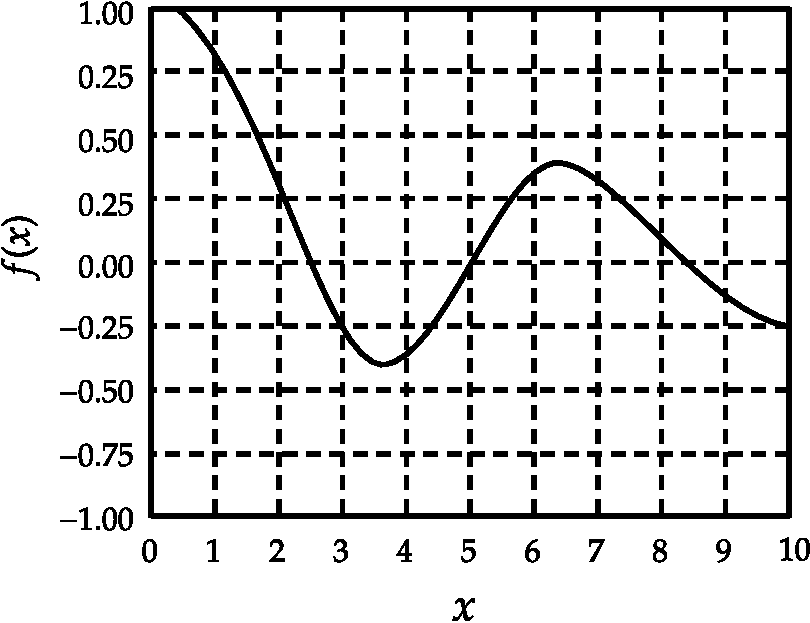
\includegraphics[height=6cm,width=8cm]{diagram-20211005(12)-crop}
	\end{figure}
	\begin{tasks}(2)
		\task[\textbf{A.}]  The Bessel function $J_{0}(x)$
		\task[\textbf{B.}] $\cos x$
		\task[\textbf{C.}] $e^{-x} \cos x$
		\task[\textbf{D.}] $\frac{1}{x} \cos x$
	\end{tasks}
	\item Given that $\sum_{n=0}^{\infty} H_{n}(x) \frac{t^{n}}{n !}=e^{-t^{2}+2 t x}$ the value of $H_{4}(0)$ is
	{\exyear{NET/JRF(JUNE-2013)}}
	\begin{tasks}(4)
		\task[\textbf{A.}] 12
		\task[\textbf{B.}] 6
		\task[\textbf{C.}] 24
		\task[\textbf{D.}] $-6$
	\end{tasks}
	\item   Given $\sum_{n=0}^{\infty} P_{n}(x) t^{n}=\left(1-2 x t+t^{2}\right)^{-1 / 2}$, for $|t|<1$, the value of $P_{5}(-1)$ is
	{\exyear{NET/JRF(JUNE-2014)}}
	\begin{tasks}(4)
		\task[\textbf{A.}] $0.26$
		\task[\textbf{B.}] 1
		\task[\textbf{C.}] $0.5$
		\task[\textbf{D.}] $-1$
	\end{tasks}
	\item The function $f(x)=\sum_{n=0}^{\infty} \frac{(-1)^{n}}{n !(n+1) !}\left(\frac{x}{2}\right)^{2 n+1}$, satisfies the differential equation
	{\exyear{NET/JRF(DEC-2014)}}
	\begin{tasks}(2)
		\task[\textbf{A.}]  $x^{2} \frac{d^{2} f}{d x^{2}}+x \frac{d f}{d x}+\left(x^{2}+1\right) f=0$
		\task[\textbf{B.}]  $x^{2} \frac{d^{2} f}{d x^{2}}+2 x \frac{d f}{d x}+\left(x^{2}-1\right) f=0$
		\task[\textbf{C.}] $x^{2} \frac{d^{2} f}{d x^{2}}+x \frac{d f}{d x}+\left(x^{2}-1\right) f=0$
		\task[\textbf{D.}] $x^{2} \frac{d^{2} f}{d x^{2}}-x \frac{d f}{d x}+\left(x^{2}-1\right) f=0$
	\end{tasks}
	\item
	 The Hermite polynomial $H_{n}(x)$, satisfies the differential equation
	$$
	\frac{d^{2} H_{n}}{d x^{2}}-2 x \frac{d H_{n}}{d x}+2 n H_{n}(x)=0
	$$
	The corresponding generating function $G(t, x)=\sum_{n=0}^{\infty} \frac{1}{n !} H_{n}(x) t^{n}$, satisfies the equation
	{\exyear{NET/JRF(DEC-2015)}}
	\begin{tasks}(2)
		\task[\textbf{A.}] $\frac{\partial^{2} G}{\partial x^{2}}-2 x \frac{\partial G}{\partial x}+2 t \frac{\partial G}{\partial t}=0$
		\task[\textbf{B.}] $\frac{\partial^{2} G}{\partial x^{2}}-2 x \frac{\partial G}{\partial x}-2 t^{2} \frac{\partial G}{\partial t}=0$
		\task[\textbf{C.}] $\frac{\partial^{2} G}{\partial x^{2}}-2 x \frac{\partial G}{\partial x}+2 \frac{\partial G}{\partial t}=0$
		\task[\textbf{D.}]  $\frac{\partial^{2} G}{\partial x^{2}}-2 x \frac{\partial G}{\partial x}+2 \frac{\partial^{2} G}{\partial x \partial t}=0$
	\end{tasks}
	\item A stable asymptotic solution of the equation $x_{n+1}=1+\frac{3}{1+x_{n}}$ is $x=2$. If we take $x_{n}=2+\epsilon_{n}$ and $x_{n+1}=2+\epsilon_{n+1}$, where $\epsilon_{n}$ and $\epsilon_{n+1}$ are both small, the ratio $\frac{\epsilon_{n+1}}{\epsilon_{n}}$ is approximately
	{\exyear{NET/JRF(DEC-2016)}}
	\begin{tasks}(4)
		\task[\textbf{A.}] $-\frac{1}{2}$
		\task[\textbf{B.}] $-\frac{1}{4}$
		\task[\textbf{C.}]  $-\frac{1}{3}$
		\task[\textbf{D.}] $-\frac{2}{3}$
	\end{tasks}
	\item  The Green's function satisfying
	$$
	\frac{d^{2}}{d x^{2}} g\left(x, x_{0}\right)=\delta\left(x-x_{0}\right)
	$$
	with the boundary conditions $g\left(-L, x_{0}\right)=0=g\left(L, x_{0}\right)$, is
	{\exyear{NET/JRF(JUNE-2017)}}
	\begin{tasks}(1)
		\task[\textbf{A.}] $\left\{\begin{array}{ll}\frac{1}{2 L}\left(x_{0}-L\right)(x+L), & -L \leq x<x_{0} \\ \frac{1}{2 L}\left(x_{0}+L\right)(x-L), & x_{0} \leq x \leq L\end{array}\right.$
		\task[\textbf{B.}]  $\left\{\begin{array}{ll}\frac{1}{2 L}\left(x_{0}+L\right)(x+L), & -L \leq x<x_{0} \\ \frac{1}{2 L}\left(x_{0}-L\right)(x-L), & x_{0} \leq x \leq L\end{array}\right.$
		\task[\textbf{C.}] $\left\{\begin{array}{ll}\frac{1}{2 L}\left(L-x_{0}\right)(x+L), & -L \leq x<x_{0} \\ \frac{1}{2 L}\left(x_{0}+L\right)(L-x), & x_{0} \leq x \leq L\end{array}\right.$
		\task[\textbf{D.}] $\frac{1}{2 L}(x-L)(x+L), \quad-L \leq x \leq L$
	\end{tasks}
	\item  The generating function $G(t, x)$ for the Legendre polynomials $P_{n}(t)$ is
	$$
	G(t, x)=\frac{1}{\sqrt{1-2 x t+x^{2}}}=\sum_{n=0}^{\infty} x^{n} P_{n}(t), \text { for }|x|<1
	$$
	If the function $f(x)$ is defined by the integral equation $\int_{0}^{x} f\left(x^{\prime}\right) d x^{\prime}=x G(1, x)$, it can be expressed as
	{\exyear{NET/JRF(DEC-2017)}}
	\begin{tasks}(2)
		\task[\textbf{A.}] $\sum_{n, m=0}^{\infty} x^{n+m} P_{n}(1) P_{m}\left(\frac{1}{2}\right)$
		\task[\textbf{B.}] $\sum_{n, m=0}^{\infty} x^{n+m} P_{n}(1) P_{m}(1)$
		\task[\textbf{C.}] $\sum_{n, m=0}^{\infty} x^{n-m} P_{n}(1) P_{m}(1)$
		\task[\textbf{D.}] $\sum_{n, m=0}^{\infty} x^{n-m} P_{n}(0) P_{m}(1)$
	\end{tasks}
	\item In the function $P_{n}(x) e^{-x^{2}}$ of a real variable $x, P_{n}(x)$ is polynomial of degree $n$. The maximum number of extrema that this function can have is
	{\exyear{NET/JRF(JUNE-2018)}}
	\begin{tasks}(4)
		\task[\textbf{A.}] $n+2$
		\task[\textbf{B.}]  $n-1$
		\task[\textbf{C.}] $n+1$
		\task[\textbf{D.}] $n$
	\end{tasks}
	\item  The Green's function $G\left(x, x^{\prime}\right)$ for the equation $\frac{d^{2} y(x)}{d x^{2}}+y(x)=f(x)$, with the boundary values $y(0)=y\left(\frac{\pi}{2}\right)=0$, is
	{\exyear{NET/JRF(JUNE-2018)}}
	\begin{tasks}(1)
		\task[\textbf{A.}] $G\left(x, x^{\prime}\right)=\left\{\begin{array}{ll}x\left(x^{\prime}-\frac{\pi}{2}\right), & 0<x<x^{\prime}<\frac{\pi}{2} \\ \left(x-\frac{\pi}{2}\right) x^{\prime}, & 0<x^{\prime}<x<\frac{\pi}{2}\end{array}\right.$
		\task[\textbf{B.}] $G\left(x, x^{\prime}\right)=\left\{\begin{array}{ll}-\cos x^{\prime} \sin x, & 0<x<x^{\prime}<\frac{\pi}{2} \\ -\sin x^{\prime} \cos x, & 0<x^{\prime}<x<\frac{\pi}{2}\end{array}\right.$
		\task[\textbf{C.}] $G\left(x, x^{\prime}\right)=\left\{\begin{array}{ll}\cos x^{\prime} \sin x, & 0<x<x^{\prime}<\frac{\pi}{2} \\ \sin x^{\prime} \cos x, & 0<x^{\prime}<x<\frac{\pi}{2}\end{array}\right.$
		\task[\textbf{D.}] $G\left(x, x^{\prime}\right)=\left\{\begin{array}{ll}x\left(\frac{\pi}{2}-x^{\prime}\right), & 0<x<x^{\prime}<\frac{\pi}{2} \\ x^{\prime}\left(\frac{\pi}{2}-x\right), & 0<x^{\prime}<x<\frac{\pi}{2}\end{array}\right.$
	\end{tasks}
	\item The polynomial $f(x)=1+5 x+3 x^{2}$ is written as linear combination of the Legendre polynomials
	$\left(P_{0}(x)=1, P_{1}(x), P_{2}(x)=\frac{1}{2}\left(3 x^{2}-1\right)\right)$ as $f(x)=\sum_{n} c_{n} P_{n}(x)$. The value of $c_{0}$ is
	{\exyear{NET/JRF(DEC-2018)}}
	\begin{tasks}(4)
		\task[\textbf{A.}] $\frac{1}{4}$
		\task[\textbf{B.}] $\frac{1}{2}$
		\task[\textbf{C.}]  2
		\task[\textbf{D.}]  4
	\end{tasks}
	\item The Green's function $G\left(x, x^{\prime}\right)$ for the equation $\frac{d^{2} y(x)}{d x^{2}}=f(x)$, with the boundary values $y(0)=0$ and $y(1)=0$, is
	{\exyear{NET/JRF(DEC-2018)}}
	\begin{tasks}(1)
		\task[\textbf{A.}] $G\left(x, x^{\prime}\right)=\left\{\begin{array}{ll}\frac{1}{2} x\left(1-x^{\prime}\right), & 0<x<x^{\prime}<1 \\ \frac{1}{2} x^{\prime}(1-x) & 0<x^{\prime}<x<1\end{array}\right.$
		\task[\textbf{B.}] $G\left(x, x^{\prime}\right)=\left\{\begin{array}{ll}x\left(x^{\prime}-1\right), & 0<x<x^{\prime}<1 \\ x^{\prime}(1-x) & 0<x^{\prime}<x<1\end{array}\right.$
		\task[\textbf{C.}] $G\left(x, x^{\prime}\right)=\left\{\begin{array}{ll}-\frac{1}{2} x\left(1-x^{\prime}\right), & 0<x<x^{\prime}<1 \\ \frac{1}{2} x^{\prime}(1-x) & 0<x^{\prime}<x<1\end{array}\right.$
		\task[\textbf{D.}]  $G\left(x, x^{\prime}\right)=\left\{\begin{array}{ll}x\left(x^{\prime}-1\right), & 0<x<x^{\prime}<1 \\ x^{\prime}(x-1) & 0<x^{\prime}<x<1\end{array}\right.$
	\end{tasks}
	\item  The Green's function for the differential equation $\frac{d^{2} x}{d t^{2}}+x=f(t)$, satisfying the initial conditions $x(0)=\frac{d x}{d t}(0)=0$ is\\
	$$G(t, \tau)=\left\{\begin{array}{ll}0 & \text { for } \quad 0<t<\tau \\ \sin (t-\tau) & \text { for } \quad t>\tau\end{array}\right.$$\\
	The solution of the differential equation when the source $f(t)=\theta(t)$ (the Heaviside step function) is
	{\exyear{NET/JRF(JUNE-2020)}}
	\begin{tasks}(4)
		\task[\textbf{A.}] $\sin t$
		\task[\textbf{B.}] $1-\sin t$
		\task[\textbf{C.}] $1-\cos t$
		\task[\textbf{D.}] $\cos ^{2} t-1$
	\end{tasks}
\end{enumerate}
 \colorlet{ocre1}{ocre!70!}
\colorlet{ocrel}{ocre!30!}
\setlength\arrayrulewidth{1pt}
\begin{table}[H]
	\centering
	\arrayrulecolor{ocre}
	\begin{tabular}{|p{1.5cm}|p{1.5cm}||p{1.5cm}|p{1.5cm}|}
		\hline
		\multicolumn{4}{|c|}{\textbf{Answer key}}\\\hline\hline
		\rowcolor{ocrel}Q.No.&Answer&Q.No.&Answer\\\hline
		1&\textbf{D} &2&\textbf{D}\\\hline 
		3&\textbf{A} &4&\textbf{A} \\\hline
		5&\textbf{D} &6&\textbf{C} \\\hline
		7&\textbf{A}&8&\textbf{C}\\\hline
		9&\textbf{A}&10&\textbf{B}\\\hline
		11&\textbf{C} &12&\textbf{B}\\\hline
		13&\textbf{C}&14&\textbf{D}\\\hline
		15&\textbf{C}& &\\\hline
		
	\end{tabular}
\end{table}
\begin{abox}
	Problem Set -3
\end{abox}
\begin{enumerate}[label=\color{ocre}\textbf{\arabic*.}]
	\item Green function for time dependent Schrödinger wave equation is defined as $G\left(\vec{r}, t: r^{\prime}, t^{\prime}\right)$. If $H$ is Hamiltonion of system then $G\left(\vec{r}, t: r^{\prime}, t^{\prime}\right)$ will satisfied the equation
	 \begin{tasks}(1)
		\task[\textbf{a.}]$\left(i \hbar \frac{\partial}{\partial t}-H\right) G\left(\vec{r}, t ; \vec{r}^{\prime}, t^{\prime}\right)=0$
		\task[\textbf{b.}]$\left(i \hbar \frac{\partial}{\partial t}-H\right) G\left(\vec{r}, t ; \vec{r}^{\prime}, t^{\prime}\right)=\delta\left(\vec{r}-\vec{r}^{\prime}\right)$
		\task[\textbf{c.}] $\left(i \hbar \frac{\partial}{\partial t}-H\right) G\left(\vec{r}, t ; \vec{r}^{\prime}, t^{\prime}\right)=\delta\left(t-t^{\prime}\right)$
		\task[\textbf{d.}]  $\left(i \hbar \frac{\partial}{\partial t}-H\right) G\left(\vec{r}, t ; \vec{r}^{\prime}, t^{\prime}\right)=\delta\left(\vec{r}-\vec{r}^{\prime}\right) \delta\left(t-t^{\prime}\right)$
	\end{tasks}
\begin{answer}
So the correct answer is \textbf{Option (d)}
\end{answer}
	\item $G\left(x, x_{0}\right)$ is the Green's function associated with the boundary value problem consisting of ordinary differential equation.
	$$
	\frac{d}{d x}\left(p(x) \frac{d u}{d x}\right)=f(x) \text { with } u(0)=0, u(L)=0
	$$
	The discontinuity condition on the derivative $\frac{d G\left(x, x_{0}\right)}{d x}$ at $x=x_{0}$ is
	 \begin{tasks}(4)
		\task[\textbf{a.}]0
		\task[\textbf{b.}]$p\left(x_{0}\right)$
		\task[\textbf{c.}]1
		\task[\textbf{d.}] $\frac{1}{p\left(x_{0}\right)}$
	\end{tasks}
\begin{answer}
	\begin{align*}
	\left.\frac{d G}{d x}\right|_{x=x_{0}^{+}}-\left.\frac{d G}{d x}\right|_{x=x_{i 1}^{-}}=\frac{1}{p\left(x_{0}\right)}
	\end{align*}
	So the correct answer is \textbf{Option (d)}
\end{answer}
\item Consider the steady state heat equation $\frac{d^{2} u}{d x^{2}}=f(x)$ with boundary condition,
$$
u(0)=0, u(L)=0
$$
The Green's function associated with the above equation
 \begin{tasks}(2)
	\task[\textbf{a.}]Constant
	\task[\textbf{b.}] Linear function
	\task[\textbf{c.}] Parabolic function
	\task[\textbf{d.}] Hyperbolic function
\end{tasks}
\begin{answer}
	\begin{align*}
	\intertext{The Green's function satisfies}
	\frac{d^{2} G\left(x, x_{0}\right)}{d x^{2}}&=\delta\left(x-x_{0}\right)\\
\text{	with }G\left(0, x_{0}\right)&=0\text{ and }G\left(L, x_{0}\right)=0
\intertext{Corresponding homogeneous equation is:}
\frac{d^{2} G}{d x^{2}}&=0\\
\text{Solution for }x \neq x_{0}&\text{ are, }G\left(x, x_{0}\right)= \begin{cases}a+b x_{2} & x<x_{1+} \\ c+d x, & x>x_{0}\end{cases}
	\end{align*}
		So the correct answer is \textbf{Option (b)}
\end{answer}
\item Consider the steady state heat equation $\frac{d^{2} u}{d x^{2}}=f(x)$ with boundary condition. $u(0)=0, u(L)=0$
The Green's function associated with the above equation is
 \begin{tasks}(1)
	\task[\textbf{a.}] $G\left(x, x_{0}\right)= \begin{cases}\frac{x}{L}\left(x_{0}-L\right), & 0 \leq x \leq x_{0} \\ \frac{x_{0}}{L}(x-L), & x_{0} \leq x \leq L\end{cases}$
	\task[\textbf{b.}] $G\left(x, x_{0}\right)= \begin{cases}\frac{x}{L}\left(L-x_{0}\right), & 0 \leq x \leq x_{0} \\ \frac{x_{0}}{L}(L-x), & x_{0} \leq x \leq L\end{cases}$
	\task[\textbf{c.}] $G\left(x, x_{0}\right)= \begin{cases}\sqrt{\frac{x}{L},} &\quad 0 \leq x \leq x_{0} \\ \sqrt{\frac{(x-L)}{L}}, & \quad x_{0} \leq x \leq L\end{cases}$
	\task[\textbf{d.}] $G\left(x, x_{0}\right)= \begin{cases}\sqrt{\frac{L-x}{L},}, & 0 \leq x \leq x_{0} \\ \sqrt{\frac{(x)}{L}}, & x_{0} \leq x \leq L\end{cases}$
\end{tasks}
\begin{answer}
	\begin{align*}
	\intertext{The Green's function satisfies}
	\frac{d^{2} G\left(x, x_{0}\right)}{d x^{2}}&=\delta\left(x-x_{0}\right)\\
	\text{with }G\left(0, x_{0}\right)&=0\text{ and }G\left(L, x_{0}\right)=0
	\intertext{Corresponding homogeneous equation is:}
	\frac{d^{2} G}{d x^{2}}&=0\\
	\text{Solution for }&x \neq x_{0}\text{ are}\\
	G\left(x, x_{0}\right)&= \begin{cases}a+b x, & x<x_{0} \\ c+d x, & x>x_{0}\end{cases}
	\intertext{From boundary conditions:}
	G\left(0, x_{0}\right)&=0 \Rightarrow a=0\\
	G\left(L, x_{0}\right)&=0 \Rightarrow c=-d L\\
	\therefore G\left(x, x_{0}\right)&= \begin{cases}b x, & x<x_{0} \\ d(x-L), & x>x_{0}\end{cases}\\
	\text{From continuity of }&\text{Green's function at }x=x_{0},\text{ we have}\\
	b x_{0}&=d\left(x_{0}-L\right)\\
	b&=\frac{d\left(x_{0}-L\right)}{x_{0}}\\
	\text{From discontinuity of }&\frac{\partial G}{\partial x}\text{ at }x=x_{0}\text{, we have}\\
	\left.\frac{\partial G}{\partial x}\right|&_{x=x_{0}^{+}}-\left.\frac{\partial G}{\partial x}\right|_{x=x_{0}^{-}}=1\\
	d-b&=1\\
	\Rightarrow d&=b+1 \Rightarrow d=\frac{d\left(x_{0}-L\right)}{x_{0}}+1 \Rightarrow d x_{0}=d x_{0}-d L+x_{0}\\
	\Rightarrow d&=\frac{x_{0}}{L}, b=d-1=\left(\frac{x_{0}}{L}-1\right)\\
	\therefore G\left(x, x_{0}\right)&= \begin{cases}\frac{x}{L}\left(x_{0}-L\right), & 0 \leq x \leq x_{0} \\ \frac{x_{0}}{L}(x-L), & x_{0} \leq x \leq L\end{cases}
	\end{align*}
		So the correct answer is \textbf{Option (a)}
\end{answer}
\item The differential equation defined as $\frac{d^{2} y}{d x^{2}}=f(x)$ With boundary conditions $\quad y(0)=0$ and $y^{\prime}(1)=0$
The green function $G\left(x, x_{0}\right)$ satisfy the
 \begin{tasks}(2)
	\task[\textbf{a.}]$G\left(x, x_{0}\right)= \begin{cases}x & \text { if } x<x_{0} \\ x_{0} & \text { if } x>x_{0}\end{cases}$
	\task[\textbf{b.}]$G\left(x, x_{0}\right)= \begin{cases}-x & \text { if } x<x_{0} \\ -x_{0} & \text { if } x>x_{0}\end{cases}$
	\task[\textbf{c.}]$G\left(x, x_{0}\right)= \begin{cases}x^{2} & \text { if } x<x_{0} \\ -x_{0} & \text { if } x>x_{0}\end{cases}$
	\task[\textbf{d.}] $G\left(x, x_{0}\right)= \begin{cases}-x^{2} & \text { if } x<x_{0} \\ -x_{0} & \text { if } x>x_{0}\end{cases}$
\end{tasks}
\begin{answer}
	\begin{align}
	\intertext{The corresponding non-homogenous differential equation for Green's function is}\notag\\
	\frac{\partial^{2}}{\partial x^{2}} G\left(x, x_{0}\right)&=\delta\left(x-x_{0}\right)\\
	\text{With }G\left(0, x_{0}\right)&=0\text{ and }G^{\prime}\left(1, x_{0}\right)=0\notag\notag\\
\text{	Let }&\frac{\partial^{2}}{\partial x^{2}} G\left(x, x_{0}\right)=0\notag\\
\Rightarrow G\left(x, x_{0}\right)&= \begin{cases}A x+B, & x<x_{0} \\ C x+D, & x>x_{0}\end{cases}\label{SF-01}
\intertext{Using booundary condition, we have}\notag\\
B&=0\text{ and }C=0\notag\\
\therefore&\text{ equation (\ref{SF-01}) becomes}\notag\\
G\left(x, x_{b}\right)&= \begin{cases}A x, & x<x_{0} \\ D, & x>x_{i 1}\end{cases}\notag\\
\text{From continuity of }&\left(f\left(x, x_{0}\right)\right.\text{ at }x=x_{0}\text{, we have}\notag\\
A x_{0}&=D
\intertext{From discontinuity of first derivative of Green's function i.c. $\frac{\partial G}{\partial x}$ at $x=x_{0}$ we have}
\left.\frac{\partial G}{\partial x}\right|_{x=x_{0}^{+}}-\left.\frac{\partial G}{\partial x}\right|&_{x=x_{0}^{-}}=1\notag\\
\Rightarrow 0-A&=1 \Rightarrow A=-1\notag\\
\text{and }D&=-x_{0}\notag\\
\therefore G\left(x, x_{0}\right)&= \begin{cases}-x & \text { if } x<x_{0} \notag\\ -x_{0} & \text { if } x>x_{0}\end{cases}
	\end{align}
	So the correct answer is \textbf{Option (b)}
\end{answer}
\item For real $n$ the cylindrical Bessel function of order $n$ is $J_{n}(x)$ then $J_{1 / 2}$ will converge to
 \begin{tasks}(4)
	\task[\textbf{a.}]0
	\task[\textbf{b.}]1
	\task[\textbf{c.}] $-1$
	\task[\textbf{d.}] $\frac{1}{2}$
\end{tasks}
\begin{answer}
	\begin{align*}
	{{\color{red}{Not completed}}}\\
	\end{align*}
	So the correct answer is \textbf{Option (a)}
\end{answer}
\item For real $n$ the cylindrical Bessel function is $J_{n}(x)$ of order $n$ then behavior $J_{1 / 2}$ will behave $x \approx 0$ as
 \begin{tasks}(4)
	\task[\textbf{a.}] 0
	\task[\textbf{b.}]$\sqrt{\frac{2 x}{\pi}}$
	\task[\textbf{c.}]$\sqrt{\frac{x}{\pi}}$
	\task[\textbf{d.}]  $\sqrt{\frac{x}{2 \pi}}$
\end{tasks}
\begin{answer}
	\begin{align*}
	{{\color{red}{Not completed}}}\\
	J_{n}(x)&=\sum_{0}^{\infty} \frac{(-1)^{r}}{[r \mid n+r}\left(\frac{x}{2}\right)^{n+2 r} \Rightarrow J_{1 / 2}(x)=\sum_{0}^{\infty} \frac{(-1)^{r}}{\left\lfloor\frac{1}{2}+r\right.}\left(\frac{x}{2}\right)^{\frac{1}{2}+2 r}\\
	\text{Put }r&=0 \frac{\sqrt{x / 2}}{\frac{1}{2}}=\sqrt{\frac{2 x}{\pi}} \text{where }\frac{1}{2}=\frac{\sqrt{\pi}}{2}
	\end{align*}
		So the correct answer is \textbf{Option (b)}
\end{answer}
\item For real $n$ the cylindrical Bessel function is $J_{n}(x)$ of order $n$ then behavior $J_{1 / 2}$ will equivalent to (it is given that $\underline{r} \cdot\left\lfloor r-\frac{1}{2}=\left[(2 r) 2^{-r} \sqrt{\pi}\right)\right.$
 \begin{tasks}(4)
	\task[\textbf{a.}] $\sqrt{\frac{2}{\pi}} \frac{\sin x}{\sqrt{x}}$
	\task[\textbf{b.}]$\sqrt{\frac{2}{\pi}} \frac{\sin x}{x}$
	\task[\textbf{c.}]$\sqrt{\frac{2}{\pi}} \frac{\cos x}{\sqrt{x}}$
	\task[\textbf{d.}] $\sqrt{\frac{2}{\pi}} \frac{\cos }{x}$
\end{tasks} 
\begin{answer}
	\begin{align*}
	{{\color{red}{Not completed}}}\\
	\end{align*}
\end{answer}
\item For real $n$ the cylindrical Bessel function is $J_{n}(x)$ of order $n$ then $J_{n}(x)$ will satisfied differential equation
 \begin{tasks}(1)
	\task[\textbf{a.}]$\frac{d^{2} J_{n}}{d x^{2}}+\frac{1}{x}\left(\frac{d J_{n}}{d x}\right)+\left(1+\frac{n^{2}}{x^{2}}\right) J_{n}=0$
	\task[\textbf{b.}] $\frac{d^{2} J_{n}}{d x^{2}}+\frac{1}{x}\left(\frac{d J_{n}}{d x}\right)+\left(1-\frac{n^{2}}{x^{2}}\right) J_{n}=0$
	\task[\textbf{c.}] $\frac{d^{2} J_{n}}{d x^{2}}+x\left(\frac{d J_{n}}{d x}\right)+\left(1+\frac{n^{2}}{x^{2}}\right) J_{n}=0$
	\task[\textbf{d.}] $\frac{d^{2} J_{n}}{d x^{2}}+x\left(\frac{d J_{n}}{d x}\right)+\left(1-\frac{n^{2}}{x^{2}}\right) J_{n}=0$
\end{tasks}
\begin{answer}
	\begin{align*}
\text{The Bessel function is given by }\frac{d^{2} J_{n}}{d x^{2}}+\frac{1}{x}\left(\frac{d J_{n}}{d x}\right)+\left(1-\frac{n^{2}}{x^{2}}\right) J_{n}=0
	\end{align*}
		So the correct answer is \textbf{Option (b)}
\end{answer}
\item For real $n$ the cylindrical Bessel function is $J_{n}(x)$ of order $n$ then value of $\frac{d J_{0}}{d x}$ is equivalent to 
 \begin{tasks}(4)
	\task[\textbf{a.}] $J_{1}$
	\task[\textbf{b.}]$-J_{1}$
	\task[\textbf{c.}]$2 J_{1}$
	\task[\textbf{d.}]$-2 J_{1}$
\end{tasks}
\begin{answer}
	\begin{align*}
J_{n+1}(x)=-J_{n}^{\prime}(x)+\frac{n}{x} J_{n}\text{. for }n=0, J_{1}=-J_{0}^{\prime}
	\end{align*}
		So the correct answer is \textbf{Option (b)}
\end{answer}
\item  The differential equation $x^{2} \frac{d^{2} y}{d x^{2}}+2 x \frac{d y}{d x}+\left[x^{2}-\lambda\right] y(x)=0$ is spherical Bessel's differential equation of order $n$ then value of $\lambda$ is given by
 \begin{tasks}(4)
	\task[\textbf{a.}]$n$
	\task[\textbf{b.}]$n(n+1)$
	\task[\textbf{c.}] $n(n-1)$
	\task[\textbf{d.}]  $n^{2}$
\end{tasks}
\begin{answer}
	\begin{align*}
\text{Spherical Bessel's differential equation }x^{2} \frac{d^{2} y}{d x^{2}}+2 x \frac{d y}{d x}+\left[x^{2}-n(n+1)\right] y(x)=0
	\end{align*}
		So the correct answer is \textbf{Option (b)}
\end{answer}
\item If $J_{n}(x)$ is spherical Bessel function of order $n$ if $N_{n}(x)$ is spherical Neumann function of order $n$ and $h_{n}^{\prime}$ is spherical Hankel function of type one of order $n$. Then $h_{0}^{1}$ is given by
 \begin{tasks}(4)
	\task[\textbf{a.}]$i \frac{e^{-i x}}{x}$
	\task[\textbf{b.}]$-i \frac{e^{-i x}}{x}$
	\task[\textbf{c.}] $i \frac{e^{i x}}{x}$
	\task[\textbf{d.}] $-i \frac{e^{i x}}{x}$
\end{tasks}
\begin{answer}
	\begin{align*}
		h_{n}^{1}&=J_{n}+i N_{n}\\
	J_{0}(x)&=\frac{\sin x}{x}, N_{0}(x)=-\frac{\cos x}{x} \Rightarrow h_{0}^{\prime^{\prime}}=J_{0}+i N_{0}=\frac{\sin x-i \cos x}{\because x}=-i \frac{e^{i x}}{x}
	\end{align*}
	So the correct answer is \textbf{Option (d)}
\end{answer}
\item If $J_{n}(x)$ is spherical Bessel function of order $n$ if $N_{n}(x)$ is spherical Neumann function of order $n$ and $h_{n}^{2}$ is spherical Hankel function of type two of order $n$. Then $h_{0}^{2}$ is given by
 \begin{tasks}(4)
	\task[\textbf{a.}] $i \frac{e^{-i x}}{x}$
	\task[\textbf{b.}] $-i \frac{e^{-i x}}{x}$
	\task[\textbf{c.}]$i \frac{e^{i x}}{x}$
	\task[\textbf{d.}] $-i \frac{e^{i x}}{x}$
\end{tasks}
\begin{answer}
	\begin{align*}
	h_{n}^{2}&=J_{n}-i N_{n}\\
	J_{0}(x)&=\frac{\sin x}{x},N_{0}(x)=-\frac{\cos x}{x} \Rightarrow h_{0}^{1}=J_{0}+i N_{0} \Rightarrow \frac{\sin x+i \cos x}{x}=i \frac{e^{-i x}}{x}
	\end{align*}
		So the correct answer is \textbf{Option (a)}
\end{answer}
\item If $J_{n}(x)$ is spherical Bessel function of order $n$ then $j_{0}^{\prime}(x)$ is equivalent to
 \begin{tasks}(4)
	\task[\textbf{a.}]$j_{1}(x)$
	\task[\textbf{b.}]$-j_{1}(x)$
	\task[\textbf{c.}]$\frac{j_{1}(x)}{2}$
	\task[\textbf{d.}]$-\frac{j_{1}(x)}{2}$
\end{tasks}
\begin{answer}
	\begin{align*}
	\frac{d}{d x}\left(j_{0}(x)\right)&=\frac{d}{d x}\left(\frac{\sin x}{x}\right)=\frac{\cos x}{x}-\frac{\sin x}{x^{2}}=-J_{1}(x)\\
	\text{Where }j_{1}(x)&=-\frac{\cos x}{x}+\frac{\sin x}{x^{2}}
	\end{align*}
	So the correct answer is \textbf{Option (b)}
\end{answer}
\item The solution of the differential equation $x^{2} \frac{d^{2} y}{d x^{2}}+2 x \frac{d y}{d x}+x^{2} y(x)=0$ subjected to the condition is given by $y(0)=1$.
 \begin{tasks}(4)
	\task[\textbf{a.}] $\frac{\sin x}{x}$
	\task[\textbf{b.}] $\frac{\cos x}{x}$
	\task[\textbf{c.}]$\frac{\exp (-i x)}{x}$
	\task[\textbf{d.}] $\frac{\exp i x}{x}$
\end{tasks}
\begin{answer}
	\begin{align*}
 \text{Spherical Bessel's differential equation }&x^{2} \frac{d^{2} y}{d x^{2}}+2 x \frac{d y}{d x}+\left[x^{2}-n(n+1)\right] y(x)=0\\
 \text{ then }x^{2} \frac{d^{2} y}{d x^{2}}+2 x \frac{d y}{d x}+x^{2} y(x)=0 &\text{ is spherical Bessel's differential equation for order}\\
 n&=0\\
	\text{then solution is }J_{0}(x)&=\frac{\sin x}{x}\text{ with boundary condition }y(0)=1.
	\end{align*}
	So the correct answer is \textbf{Option (a)}
\end{answer}
\item $H_{n}(x)$ is Hermite polynomials of order $n$ then $H_{n}(x)=(-1)^{n} f(x) \frac{d^{n}(W(x))}{d x^{n}}$, then $f(x)$ and $W(x)$ are respectively
 \begin{tasks}(1)
	\task[\textbf{a.}]$f(x)=\exp \left(x^{2}\right), W(x)=\exp \left(-x^{2}\right)$
	\task[\textbf{b.}]$f(x)=\exp \left(-x^{2}\right), W=\exp \left(x^{2}\right)$
	\task[\textbf{c.}] $f(x)=W(x)=\exp \left(x^{2}\right)$
	\task[\textbf{d.}] $f(x)=W(x)=\exp \left(-x^{2}\right)$
\end{tasks}
\begin{answer}
	\begin{align*}
	H_{n}(x)&=(-1)^{n} \exp \left(x^{2}\right) \frac{d^{n}\left(\exp \left(-x^{2}\right)\right)}{d x^{n}}\\
	\text{So after comparing }H_{n}(x)&=(-1)^{n} f(x) \frac{d^{n}(W(x))}{d x^{n}}\\
	f(x)&=\exp \left(x^{2}\right), W(x)=\exp \left(-x^{2}\right)
	\end{align*}
		So the correct answer is \textbf{Option (a)}
\end{answer}
\item The solution of differential equation $\frac{d^{2} y}{d x^{2}}-2 x \frac{d y}{d x}+\lambda y(x)=0$ is Hermilte polynomial of order $n$ then value of $\lambda$ is
 \begin{tasks}(4)
	\task[\textbf{a.}]$n$
	\task[\textbf{b.}] $-n$
	\task[\textbf{c.}]$2 n$
	\task[\textbf{d.}] $-2 n$
\end{tasks}
\begin{answer}
	\begin{align*}
	\frac{d^{2} y}{d x^{2}}-2 x \frac{d y}{d x}+2 n y(x)=0\text{ is Hermite differential equation}
	\end{align*}
		So the correct answer is \textbf{Option (c)}
\end{answer}
\item The Rodrigues formula for Laguerre polunomial is given by
 \begin{tasks}(2)
	\task[\textbf{a.}]$L_n(x)=\frac{e^{-x}}{n !}\left(\frac{d}{d x}\right)^{n}\left(x^{n} e^{-x}\right)$
	\task[\textbf{b.}]$L_{n}(x)=\frac{e^{x}}{n !}\left(\frac{d}{d x}\right)^{n}\left(x^{n} e^{x}\right)$
	\task[\textbf{c.}]$L_n(x)=\frac{e^{-x}}{n !}\left(\frac{d}{d x}\right)^{n}\left(x^{n} e^{x}\right)$
	\task[\textbf{d.}] $L_{n}(x)=\frac{e^{x}}{n !}\left(\frac{d}{d x}\right)^{n}\left(x^{n} e^{-x}\right)$
\end{tasks}
\begin{answer}
	\begin{align*}
	L_{n}(x)=\frac{e^{x}}{n !}\left(\frac{d}{d x}\right)^{n}\left(x^{n} e^{-x}\right)
	\end{align*}
		So the correct answer is \textbf{Option (d)}
\end{answer}
\item It is given that operator $x-\frac{d}{d x}=-\exp \left(\frac{x^{2}}{2}\right) \frac{d}{d x} \exp \left(-\frac{x^{2}}{2}\right)$
If then the normalized wave function for harmonic oscillation is $\psi(x)=\left(\pi^{1 / 2} 2^{n}\lfloor n)^{-1 / 2} \exp \left(-\frac{x^{2}}{2}\right) H_{n}(x)\right.$, then $\psi_n(x)$ is equivalent to 
 \begin{tasks}(1)
	\task[\textbf{a.}]$\psi_{n}(x)=\left(\pi^{1 / 2} 2^{n}\lfloor n)^{-1 / 2}\left(x-\frac{d}{d x}\right)^{n} \exp \left(-\frac{x^{2}}{2}\right)\right.$
	\task[\textbf{b.}] $\psi_{n}(x)=\left(\pi^{1 / 2} 2^{n}\lfloor n)^{-1 / 2}\left(x-\frac{d}{d x}\right)^{2 n} \exp \left(\frac{x^{2}}{2}\right)\right.$
	\task[\textbf{c.}] $\psi_{n}(x)=\left(\pi^{1 / 2} 2^{n}\lfloor n)^{-1 / 2}\left(x-\frac{d}{d x}\right)^{n} \exp \left(-x^{2}\right)\right.$
	\task[\textbf{d.}] $\psi_{n}(x)=\left(\pi^{k / 2} 2^{n}\lfloor n)^{-1 / 2}\left(x-\frac{d}{d x}\right)^{2 n} \operatorname{cxp}\left(-x^{2}\right)\right.$
\end{tasks}
\begin{answer}
	\begin{align*}
	H_{n}(x)&=(-1)^{n} \exp \left(x^{2}\right) \frac{d^{n}\left(\exp \left(-x^{2}\right)\right)}{d x^{n}}\\
	x-\frac{d}{d x} &=-\exp \left(\frac{x^{2}}{2}\right) \frac{d}{d x} \exp \left(-\frac{x^{2}}{2}\right) \Rightarrow\left(x-\frac{d}{d x}\right) \exp \left(-\frac{x^{2}}{2}\right) \\ &\left.=-\exp \left(\frac{x^{2}}{2}\right) \frac{d}{d x} \exp \left(-\frac{x^{2}}{2}\right)\right) \exp \left(-\frac{x^{2}}{2}\right)\\
	x \exp \left(-\frac{x^{2}}{2}\right)-\frac{d \exp \left(-\frac{x^{2}}{2}\right)}{d x}&=-\exp \left(\frac{x^{2}}{2}\right) \frac{d}{d x} \exp \left(-x^{2}\right)\\
	\Rightarrow\left(x-\frac{d}{d x}\right) \exp \left(-\frac{x^{2}}{2}\right)&=\exp \left(\frac{x^{2}}{2}\right)\left(-2 x \exp \left(-x^{2}\right)\right)=2 x \exp -\frac{x^{2}}{2}=H_{1}\left(\exp -\frac{x^{2}}{2}\right)\\
	\text{where }2 x&=H_{1}(x)\\
	\text{Similarly }\left(x-\frac{d}{d x}\right)^{n} \exp \left(-\frac{x^{2}}{2}\right)&=H_{n} \exp \left(-\frac{x^{2}}{2}\right)\\
	\psi_{n}(x)&=\left(\pi^{1 / 2} 2^{n}\lfloor n)^{-1 / 2}\left(x-\frac{d}{d x}\right)^{n} \exp \left(-\frac{x^{2}}{-2}\right)\right.
	\end{align*}
	So the correct answer is \textbf{Option (a)}
\end{answer}
\item The solution of differential equation $x \frac{d^{2} y}{d x^{2}}+(1-x) \frac{d y}{d x}+\lambda y(x)=0$ is Laguerre polynomials of order $n$ then value of $\lambda$ is
 \begin{tasks}(4)
	\task[\textbf{a.}]$n$
	\task[\textbf{b.}]$-n$
	\task[\textbf{c.}] $2 n$
	\task[\textbf{d.}] $-2 n$
\end{tasks}
\begin{answer}
	\begin{align*}
	x \frac{d^{2} y}{d x^{2}}+(1-x) \frac{d y}{d x}+n y(x)=0\text{ is Laguerre differential equation.}
	\end{align*}
	So the correct answer is \textbf{Option (a)}
\end{answer}
\item The generating function $F(x, t)=\sum_{n=0}^{\infty} P_{n}(x) t^{n}$ for the Legendre polynomials $P_{n}(x)$ is $F(x, t)=\left(1-2 x t+t^{2}\right)^{-1 / 2}$. The value of $P_{2}(-1)$ is
 \begin{tasks}(4)
	\task[\textbf{a.}]$5 / 2$
	\task[\textbf{b.}]$3 / 2$
	\task[\textbf{c.}] $+1$
	\task[\textbf{d.}] $-1$
\end{tasks}
\begin{answer}
	\begin{align*}
	\text{The generating function for Legendre polynomial is }F(x, t)&=\left(1-2 x t+t^{2}\right)^{-1 / 2}.\text{ Thus}\\P_{2}(x)=\frac{1}{2}\left(3 x^{2}-1\right) \Rightarrow P_{2}(-1)=\frac{1}{2}(3-1)=1
	\end{align*}
		So the correct answer is \textbf{Option (c)}
\end{answer}
\item If we observe plot of Bessel functions $J_{0}(x), J_{1}(x)$, and $J_{2}(x)$ we find their maxima at $x_{0}, x_{1}$ and $x_{2}$ respectively. Then which of the following is true
 \begin{tasks}(2)
	\task[\textbf{a.}]$x_{0}<x_{1}<x_{2}$
	\task[\textbf{b.}]$x_{0}>x_{1}>x_{2}$
	\task[\textbf{c.}]$x_{0}<x_{1}=x_{2}$
	\task[\textbf{d.}] $x_{0}=x_{1}<x_{2}$
\end{tasks}
\begin{answer}
	So the correct answer is \textbf{Option (a)}
\end{answer}
\item Which one of the following is correctly matched?\\
\begin{figure}[H]
	\centering
	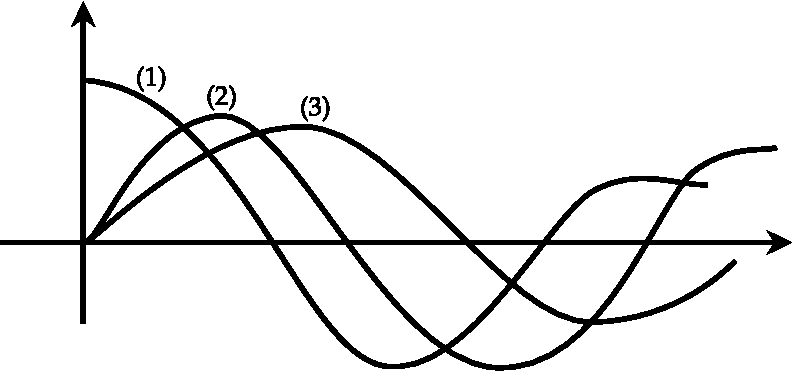
\includegraphics[height=3.5cm,width=6.5cm]{SF-01}
\end{figure}
 \begin{tasks}(2)
	\task[\textbf{a.}](1) $J_{0}$,
	(2) $J_{2}$, (3) $J_{1}$
	\task[\textbf{b.}]$(1) J_{0}$,
	(2) $J_{1}, \quad(3) J_{2}$
	\task[\textbf{c.}](1) $J_{2}$,
	(2) $J_{1}$,
	(3) $J_{0}$
	\task[\textbf{d.}] None of the above
\end{tasks}
\begin{answer}
	So the correct answer is \textbf{Option (b)}
\end{answer}
\item If the generating function of Legendre polynomial is $\frac{1}{\sqrt{1-6 t+t^{2}}}$, then coefficient of $t^{2}$ is
 \begin{tasks}(4)
	\task[\textbf{a.}] 11
	\task[\textbf{b.}]$-11$
	\task[\textbf{c.}]13
	\task[\textbf{d.}] $-13$
\end{tasks}
\begin{answer}
	\begin{align*}
	\intertext{The generating function for the polynomial solutions of the Legendre ODE is given by}
	g(x, t)&=\frac{1}{\sqrt{1-2 x t+t^{2}}}=\sum_{n=0}^{\infty} P_{n}(x) t^{n}\\
	\text{Thus }x&=3\text{ and }n=2.\\
	P_{2}(x)&=\frac{1}{2}\left(3 x^{2}-1\right) \Rightarrow P_{2}(3)=\frac{1}{2}\left(3 \times 3^{2}-1\right)=13
	\end{align*}
		So the correct answer is \textbf{Option (c)}
\end{answer}
\item Which of the following relation is true for Bessel's differential equation?
 \begin{tasks}(2)
	\task[\textbf{a.}]$J_{0}^{\prime}(x)=J_{1}(x)$
	\task[\textbf{b.}]$J_{0}^{\prime}(x)=-J_{2}(x)$
	\task[\textbf{c.}]$J_{0}^{\prime}(x)=J_{2}(x)$
	\task[\textbf{d.}] $J_{0}^{\prime}(x)=-J_{1}(x)$
\end{tasks}
\begin{answer}
	So the correct answer is \textbf{Option (d)}
\end{answer}
\item Given that $\sum_{n=0}^{\infty} H_{n}(x) \frac{t^{n}}{n !}=e^{-t^{2}+2 x x}$ the value of $H_{6}(0)$ is
 \begin{tasks}(4)
	\task[\textbf{a.}]$-120$
	\task[\textbf{b.}]$+120$
	\task[\textbf{c.}]12
	\task[\textbf{d.}]  $-12$
\end{tasks}
\begin{answer}
	\begin{align*}
	\sum_{n=0}^{\infty} I_{n}(x) \frac{t^{\prime \prime}}{n !}&=e^{-t^{2}+2 t x} \Rightarrow \sum_{n=0}^{\infty} H_{n}(0) \frac{t^{n}}{n !}=e^{-t^{2}}=1-t^{2}+\frac{t^{4}}{2 !}-\frac{t^{6}}{3 !}\\
	\Rightarrow \frac{H_{6}(0)}{6 !} t^{6}&=-\frac{1}{3 !} t^{6} \Rightarrow H_{6}(0)=-\frac{6 !}{3 !}=-120
	\end{align*}
	So the correct answer is \textbf{Option (a)}
\end{answer}
\item Given that $\sum_{n=0}^{\infty} H_{n}(x) \frac{t^{n}}{n !}=e^{-t^{2}+2 e x}$ the value of $H_{4}(0)$ is
 \begin{tasks}(4)
	\task[\textbf{a.}]12
	\task[\textbf{b.}] 6
	\task[\textbf{c.}]24
	\task[\textbf{d.}] $-6$
\end{tasks}
\begin{answer}
	\begin{align*}
	\sum_{n=0}^{\infty} H_{n}(x) \frac{t^{n}}{n !}&=e^{-t^{2}+2 t x} \Rightarrow \sum_{n=0}^{\infty} H_{n}(0) \frac{t^{n}}{n !}=e^{-t^{2}}=1-t^{2}+\frac{t^{4}}{2 !}-\frac{t^{6}}{3 !}\\
	\Rightarrow \frac{H_{4}(0)}{4 !} t^{4}&=\frac{t^{4}}{2 !} \Rightarrow H_{4}(0)=\frac{4 !}{2 !}=12
	\end{align*}
	So the correct answer is \textbf{Option (a)}
\end{answer}
\item If Hermite polynomial of order 2 is given by $H_{2}(x)=a x^{2}-2 ; a>0$, then the value of $a$ is
 \begin{tasks}(4)
	\task[\textbf{a.}]3
	\task[\textbf{b.}]4
	\task[\textbf{c.}]5
	\task[\textbf{d.}] 6
\end{tasks}
\begin{answer}
	\begin{align*}
	\intertext{Orthonormality condition,}
	\int_{-\infty}^{+\infty}\left[H_{n}(x)\right]^{2} e^{-x^{2}} d x&=2^{\prime \prime} n ! \sqrt{\pi}\\
	\text{For, }n&=2, \int_{-\infty}^{+\infty}\left(a x^{2}-2\right)^{2} e^{-x^{2}} d x=8 \sqrt{\pi}\\
\text{	Now}
	\int_{-\infty}^{+\infty}\left[H_{2}(x)\right]^{2} e^{-x^{2}} d x&=\int_{-\infty}^{+\infty}\left(a x^{2}-2\right)^{2} e^{-x^{2}} d x=\left\{a^{2} \times \frac{3}{4}+4-2 a\right\} \sqrt{\pi}
	\intertext{Thus, we have}
	\frac{3 a^{2}}{4}+4-2 a&=8 \Rightarrow 3 a^{2}-8 a-16=0 \Rightarrow 3 a^{2}-12 a+4 a-16=0\\
	\Rightarrow 3 a(a-4)+4(a-4)&=0 \Rightarrow(3 a+4)(a-4)=0\\
	\text{Thus, }a&=4
	\end{align*}
		So the correct answer is \textbf{Option (b)}
\end{answer}
\item The value of Legendre polynomial $p_{n}(x)$ for odd $n$ and $x=0$. i.e., $p_{n}(0)$ is
 \begin{tasks}(4)
	\task[\textbf{a.}]1
	\task[\textbf{b.}]0
	\task[\textbf{c.}]$-1$
	\task[\textbf{d.}]  $0.5$
\end{tasks}
\begin{answer}
	\begin{align*}
	\intertext{The generating function for Legendre polynomial is}
	\left(1-2 x t+t^{2}\right)^{-1 / 2}&=\sum_{n=0}^{\infty} p_{n}(x) t^{n}\\
	\text{Put, $x=0$, we get, }&\left(1+t^{2}\right)^{-1 / 2}=\sum p_{n}(\theta) t^{n}
	\end{align*}
		So the correct answer is \textbf{Option (b)}
\end{answer}
\item For the Legendre's polynomial $P_{n}(x)$, given below are two statements. Study these carefully and pick out the correct option.\\
Statement I: $\quad \int_{-1}^{1} x\left[P_{n}(x)\right]^{2} d x=0$\\
Statement I: $\lim _{n \rightarrow \infty}\left[\int_{-1}^{1} x P_{n}(x) P_{n+1}(x) d x\right]=0$
 \begin{tasks}(1)
	\task[\textbf{a.}]Only statement (I) is correct
	\task[\textbf{b.}]Only statement (II) is correct
	\task[\textbf{c.}]Both (I) and (II) are correct
	\task[\textbf{d.}]Neither (I) nor (II) is correet
\end{tasks}
\begin{answer}
	\begin{align*}
	\intertext{From recurrence relation we have}
	(n+1) P_{n+1}(x)&=(2 n+1) x p_{n}(x)-n p_{n-1}(x)\\
	x p_{n}(x)&=\frac{1}{(2 n+1)}\left\{(n+1) p_{n+1}(x)+n p_{n-1}(x)\right\}\\
	x\left[p_{n}(x)\right]^{2}&=\frac{1}{(2 n+1)}\left\{(n+1) p_{n}(x) p_{n+1}(x)+n p_{n}(x) p_{n-1}(x)\right\}\\
	\therefore \int_{-1}^{+1} x\left[p_{n}(x)\right]^{2} d x&=0\left\{\because \int_{-1}^{+1} p_{m}(x) p_{n}(x)=0\right.\text{ if }\left.m \neq n\right\}\\
	\therefore &\int_{-1}^{+1} x\left[p_{n}(x)\right]^{2} d x=0
	\intertext{From recurrence relation, we have}
	(n+1) p_{n+1}(x)&=(2 n+1) x p_{n}(x)-n p_{n-1}(x)\\
	(2 n+1) x p_{n}(x)&=(n+1) p_{n+1}(x)+n p_{n-1}(x)\\
	\int_{-1}^{+1}(2 n+1) x p_{n}(x) p_{n+1}(x) d x&=\int_{-1}^{+1}\left[(n+1)\left\{p_{n+1}(x)\right\}^{2}+n p_{n-1}(x) p_{n+1}(x)\right] d x\\
	=\int_{-1}^{+1}(n+1)\left\{p_{n+1}(x)\right\}^{2} d x+n \int_{-1}^{+1}& p_{n-1}(x) p_{n+1}(x) d x=(n+1) \frac{2}{2(n+1)+1}+0=\frac{2 n+2}{2 n+3}\\
	\therefore \int_{-1}^{+1} x p_{n}(x) p_{n+1}(x) d x&=\frac{2 n+2}{(2 n+1)(2 n+3)}\\
	\lim _{n \rightarrow \infty} \frac{n\left(2+\frac{2}{n}\right)}{n^{2}\left(2+\frac{1}{n}\right)\left(2+\frac{3}{n}\right)}&=\lim _{n \rightarrow \infty} \frac{\left(2+\frac{2}{n}\right)}{n\left(2+\frac{1}{n}\right)\left(2+\frac{3}{n}\right)}=0
	\end{align*}
		So the correct answer is \textbf{Option (c)}
\end{answer}
\item Which of the following statements is Incorrect about the Hermite polynomials $H_{n}(x)$ ?
 \begin{tasks}(1)
	\task[\textbf{a.}] The value of integral $\frac{1}{\sqrt{\pi}} \int_{-\infty}^{\infty} e^{-x^{2}}\left[H_{4}(x)\right]^{2} d x$ is 384
	\task[\textbf{b.}] Hermite polynomial of order $3, H_{3}(x)$, satisfies the differential equation $y^{\prime \prime}-2 x y^{\prime}+6 y=0$
	\task[\textbf{c.}] The value of $\mathrm{H}_{4}(\mathrm{l})$ is $-20$
	\task[\textbf{d.}] $H_{n}(x)=\frac{H_{n+1}(x)+2 n H_{n-1}(x)}{x}$
\end{tasks}
\begin{answer}
	\begin{align*}
	\intertext{When integrated with respect to weight function $e^{-x^{2}}$, the Hermite polynomials satisfy}
	\int_{-\infty}^{\infty} e^{-x^{2}} H_{n}(x) H_{m}(x) d x&= \begin{cases}0, & n \neq m \\ \sqrt{\pi} 2^{n} n !, & n=m\end{cases}
	\intertext{In our case $n=m=4$, hence}
	\frac{1}{\sqrt{\pi}} \int_{-\infty}^{\infty} e^{-x^{2}}\left[H_{4}(x)\right]^{2} d x&=\frac{\sqrt{\pi} 2^{4}(4 !)}{\sqrt{\pi}}=384
	\intertext{Hermite polynomial of order $n$, satisfies the differential equation}
	y^{\prime \prime}-2 x y^{\prime}+2 n y=0\\
\text{	when }n=3, y^{\prime \prime}-2 x y^{\prime}+6 y=0\\
	\text{We have }H_{4}(x)&=16 x^{4}-48 x^{2}+12\\
	\text{Therefore, }H_{4}(1)&=-48+28=-20
	\intertext{The recursion relation for Hermite polynomials is}
	H_{n+1}(x)&=2 x H_{n}(x)-2 n H_{n-1}(x) \Rightarrow H_{n}(x)=\frac{H_{n+1}(x)+2 n H_{n-1}(x)}{2 x}
	\end{align*}
		So the correct answer is \textbf{Option (d)}
\end{answer}
\item If $P_{n}(x)$ denotes the Legendre polynomials of order $n$, then which of the following statements is incorrect?
 \begin{tasks}(1)
	\task[\textbf{a.}]$P_{n}(x)=\frac{1}{2^{n} n !} \frac{d^{n}}{d x^{n}}\left[\left(x^{2}-1\right)^{n}\right]$ where $n=0,1,2 \ldots$
	\task[\textbf{b.}]The Legendre polynomials satisfy the differential equation\\$
	\left(1-x^{2}\right) \frac{d^{2} y}{d x^{2}}-2 x \frac{d y}{d x}+n(n+1) y=0
	$
	\task[\textbf{c.}] For each value of $n$ the Legendre polynomials satisfy the relation $P_{n}(1)=1$.
	\task[\textbf{d.}] The value of integral $\int_{-1}^{1}\left[P_{4}(x)\right]^{2} d x$ is $\frac{2}{7}$.
\end{tasks}
\begin{answer}
	\begin{align*}
	\intertext{Option (a) is the correct definition of Legendre polynomial. Legendre polynoimials satisfy the differential equation given in option (b). For each value of $n$ Legendre polynomials satisfy $P_{n}(1)=1$.}
	\text{Since, }\int_{-1}^{1}\left[P_{n}(x)\right]^{2} d x&=\frac{2}{2 n+1}\\
	\text{Hence, }\int_{-1}^{1}\left[P_{4}(x)\right]^{2} d x&=\frac{2}{2 \cdot 4+1}=\frac{2}{9}\\
	\text{Hence option }&(d)\text{ is incorrect.}
	\end{align*}
		So the correct answer is \textbf{Option (d)}
\end{answer}
\end{enumerate}
%\chapter{Probability Problem set Solutions}
\begin{enumerate}
	\item An unbiased die is cast twice. The probability that the positive difference (bigger smaller) between the two numbers is 2 is
	{\exyear{ JEST 2012}}
	 \begin{tasks}(2)
		\task[\textbf{a.}]$\frac{1}{9}$
		\task[\textbf{b.}]$\frac{2}{9}$
		\task[\textbf{c.}] $\frac{1}{6}$
		\task[\textbf{d.}] $\frac{1}{3}$
	\end{tasks}
	\begin{answer}
		\begin{align*}
		p(2)&=\frac{n(E)}{n(S)}
		\intertext{The number of ways to come positive difference}
		&[(3,1),(4,2),(5,3),(6,4),(1,3)(2,4),(3,5)(4,6)]\\
		p(2)&=\frac{8}{36}=\frac{2}{9}
		\end{align*}
		So the correct answer is \textbf{Option (b)}
	\end{answer}
	\item A box contains 100 coins out of which 99 are fair coins and 1 is a double-headed coin. Suppose you choose a coin at random and toss it 3 times. It turns out that the results of all 3 tosses are heads. What is the probability that the coin you have drawn is the doubleheaded one?
	{\exyear{ JEST 2013}}
	 \begin{tasks}(2)
		\task[\textbf{a.}] $0.99$
		\task[\textbf{b.}]$0.925$
		\task[\textbf{c.}] $0.75$
		\task[\textbf{d.}] $0.01$
	\end{tasks}
	\begin{answer}
		So the correct answer is \textbf{Option (c)}
	\end{answer}
	\item There are on average 20 buses per hour at a point, but at random times. The probability that there are no buses in five minutes is closest to
	{\exyear{ JEST 2013}}
	 \begin{tasks}(2)
		\task[\textbf{a.}]$0.07$
		\task[\textbf{b.}] $0.60$
		\task[\textbf{c.}]$0.36$
		\task[\textbf{d.}] $0.19$
	\end{tasks}
	\begin{answer}
		\begin{align*}
		\intertext{From Poision's distribution function,}
		P(n)&=\frac{e^{-\lambda} \lambda^{n}}{\lfloor n}
		\text{here, }\lambda&=20\text{ buses per hour }\\
		\Rightarrow \lambda&=\frac{5}{3}\text{ buses in five minutes}
		\intertext{Therefore, the probability that there are no buses in five minutes,}
		P(n=0)&=\frac{e^{-\frac{5}{3}}\left(\frac{5}{3}\right)^{0}}{\lfloor 0}=e^{-5 / 3}=0.1886 \approx 0.19
		\end{align*}
		So the correct answer is \textbf{Option (d)}
	\end{answer}
	\item Two drunks start out together at the origin, each having equal probability of making a step simultaneously to the left or right along the $x$ axis. The probability that they meet after $n$ steps is
	{\exyear{ JEST 2013}}
	 \begin{tasks}(2)
		\task[\textbf{a.}]$\frac{1}{4^{n}} \frac{2 n !}{n !^{2}}$
		\task[\textbf{b.}] $\frac{1}{2^{n}} \frac{2 n !}{n !^{2}}$
		\task[\textbf{c.}] $\frac{1}{2^{n}} 2 n !$
		\task[\textbf{d.}]  $\frac{1}{4^{n}} n !$
	\end{tasks}
	\begin{answer}
		\begin{align*}
		\text{The probability of taking ' $r$ '}&\text{ steps out of $N$ steps }={ }^{N} C_{r}\left(\frac{1}{2}\right)^{r}\left(\frac{1}{2}\right)^{N-r}\\
		\text{Total steps }&=N=n+n=2 n
	\intertext{	For taking probability of $n$ steps out of $N$}
	P={ }^{N} C_{n}\left(\frac{1}{2}\right)^{n}\left(\frac{1}{2}\right)^{N-n}&=\frac{N !}{(N-n) ! n !}\left(\frac{1}{2}\right)^{n}\left(\frac{1}{2}\right)^{N-n}=\frac{2 n !}{n ! n !}\left(\frac{1}{2}\right)^{2 n}=\frac{2 n !}{(n !)^{2} 4^{n}}
		\end{align*}
		So the correct answer is \textbf{Option (a)}
	\end{answer}
	\item If two ideal dice are rolled once, what is the probability of getting atleast one '6'?
	{\exyear{ JEST 2015}}
	 \begin{tasks}(2)
		\task[\textbf{a.}]$\frac{11}{36}$
		\task[\textbf{b.}]$\frac{1}{36}$
		\task[\textbf{c.}]$\frac{10}{36}$
		\task[\textbf{d.}]  $\frac{5}{36}$
	\end{tasks}
	\begin{answer}
		\begin{align*}
		\text{Number of point}&\text{ in sample space } n(S)=11\\
		[(1,6),(2,6),(3,6),&(4,6),(5,6),(6,1),(6,2),(6,3),(6,4),(6,5),(6,6)]\\
	\text{	Number of point }&\text{in population }n(P)=6^{2}=36
		\intertext{Probability of getting atleast one '6' on face of dice} &=\frac{n(S)}{n(P)}=\frac{11}{36}
		\end{align*}
			So the correct answer is \textbf{Option (a)}
	\end{answer}
	\item The mean value of random variable $x$ with probability density $p(x)=\frac{1}{\sigma \sqrt{2 \pi}} . \exp \left[-\frac{\left(x^{2}+\mu x\right)}{\left(2 \sigma^{2}\right)}\right]$ is:
	{\exyear{ JEST 2016}}
	 \begin{tasks}(2)
		\task[\textbf{a.}]0
		\task[\textbf{b.}]$\frac{\mu}{2}$
		\task[\textbf{c.}] $\frac{-\mu}{2}$
		\task[\textbf{d.}]  $\sigma$
	\end{tasks}
	\begin{answer}
		\begin{align*}
		\langle x\rangle=\frac{1}{\sigma \sqrt{2 \pi}} \int_{-\infty}^{\infty} x \exp \left(-\frac{x^{2}}{2 \sigma^{2}}\right) d x \int_{-\infty}^{\infty} \exp \left(-\frac{\mu x}{2 \sigma^{2}}\right) d x=0 \quad\text{ (due to odd function)}
		\end{align*}
		So the correct answer is \textbf{Option (a)}
	\end{answer}
\item Suppose that we toss two fair coins hundred times each. The probability that the same number of heads occur for both coins at the end of the experiment is
{\exyear{ JEST 2017}}
 \begin{tasks}(2)
	\task[\textbf{a.}]$\left(\frac{1}{4}\right)^{100} \sum_{n=0}^{100}\left(\begin{array}{c}100 \\ n\end{array}\right)$
	\task[\textbf{b.}] $2\left(\frac{1}{4}\right)^{100} \sum_{n=0}^{100}\left(\begin{array}{c}100 \\ n\end{array}\right)^{2}$
	\task[\textbf{c.}]$\frac{1}{2}\left(\frac{1}{4}\right)^{100} \sum_{n=0}^{100}\left(\begin{array}{c}100 \\ n\end{array}\right)^{2}$
	\task[\textbf{d.}] $\left(\frac{1}{4}\right)^{100} \sum_{n=0}^{100}\left(\begin{array}{c}100 \\ n\end{array}\right)^{2}$
\end{tasks}
\begin{answer}
	\begin{align*}
	\intertext{ If we toss one fair coins hundred times, then probability of $n$ number of head occurs at the end of 100 times is}
	&{ }^{100} C_{n}\left(\frac{1}{2}\right)^{n}\left(\frac{1}{2}\right)^{100-n}
\intertext{	Hence, the probability that same number of heads occur for both coins at the end of experiment is}
&\sum_{n=0}^{100}\left({ }^{100} C_{n}\left(\frac{1}{2}\right)^{100}\right) \cdot\left({ }^{100} C_{n}\left(\frac{1}{2}\right)^{100}\right)=\sum_{n=1}^{100}\left({ }^{100} C_{n}\right)^{2}\left(\frac{1}{2}\right)^{200}=\left(\frac{1}{4}\right)^{100} \sum_{n=1}^{100}\left({ }^{100} C_{n}\right)^{2}
	\end{align*}
		So the correct answer is \textbf{Option (d)}
\end{answer}
\item An electronic circuit with 10000 components performs its intended function success fully with a probability $0.99$ if there are no faulty components in the circuit. The probability that there are faulty components is $0.05$. if there are faulty components, the circuit perform successfully with a probability $0.3$. The probability that the circuit performs successfully is $\frac{x}{10000}$. What is $x$ ?
{\exyear{ JEST 2018}}
\begin{answer}
So the correct answer is  \textbf{9555}
\end{answer}
\item A person plans to go from town $A$ to town $B$ by taking either the route $(R 1+R 2)$ with probability $\frac{1}{2}$ or the route $(R 1+R 3)$ with probability $\frac{1}{2}$ (see figure). Further, there is a probability $\frac{1}{3}$ that $R 1$ is blocked, a probability $\frac{1}{3}$ that $R 2$ is blocked, and a probability $\frac{1}{3}$ that $R 3$ is blocked. What is the probability that he/she would reach town $B$ ?
{\exyear{ JEST 2019}}
\begin{figure}[H]
	\centering
	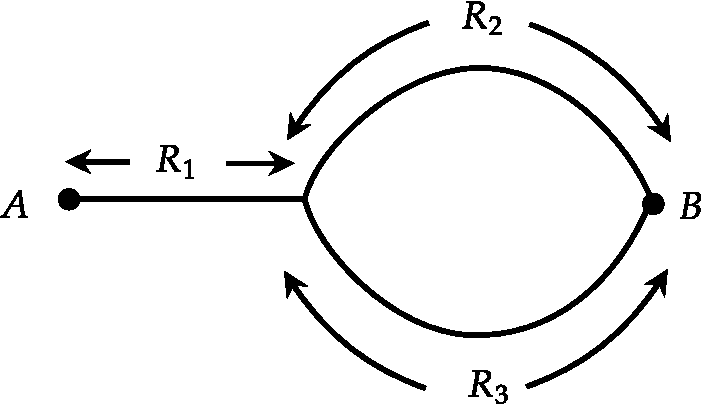
\includegraphics[height=3cm,width=5.5cm]{JEST-58-2019}
\end{figure}
 \begin{tasks}(2)
	\task[\textbf{a.}]$\frac{8}{9}$
	\task[\textbf{b.}]$\frac{1}{3}$
	\task[\textbf{c.}]$\frac{4}{9}$
	\task[\textbf{d.}]$\frac{2}{3}$
\end{tasks}
\begin{answer}
	\begin{align*}
	\text{Given that probability of}&\text{ $R 1$ blocked }=1 / 3\\
	\text{Probability of $R 1$ }&\text{not blocked }=1-\frac{1}{3}=\frac{2}{3}\\
	\text{Probability from $A$ to $B$ }&\text{without restriction }=\frac{1}{2}\\
	\text{Route $R 2$ probability }&=\frac{1}{2} \times \frac{2}{3}\text{ not blocked}\\
	\text{Route }R 3&=\frac{1}{2} \times \frac{2}{3}\\
\text{	Total probability }(A \rightarrow B)&=\frac{2}{3}\left[\frac{1}{2} \times \frac{2}{3}+\frac{1}{2} \times \frac{2}{3}\right]=\frac{4}{9}
	\end{align*}
	So the correct answer is \textbf{Option (c)}
\end{answer}

\end{enumerate}
%\chapter{title}
\newpage
\begin{abox}
	Practise Set-1
\end{abox}
\begin{enumerate}[label=\color{ocre}\textbf{\arabic*.}]
	\item An unbiased dice is thrown three times successively. The probability that the numbers of dots on the uppermost surface add up to 16 is
{\exyear{NET/JRF(DEC-2011)}}
\begin{tasks}(4)
	\task[\textbf{A.}] $\frac{1}{16}$
	\task[\textbf{B.}] $\frac{1}{36}$
	\task[\textbf{C.}] $\frac{1}{108}$
	\task[\textbf{D.}] $\frac{1}{216}$
\end{tasks}
\item A ball is picked at random from one of two boxes that contain 2 black and 3 white and 3 black and 4 white balls respectively. What is the probability that it is white?
{\exyear{NET/JRF(JUNE-2012)}}
\begin{tasks}(4)
	\task[\textbf{A.}] $34 / 70$
	\task[\textbf{B.}] $41 / 70$
	\task[\textbf{C.}] $36 / 70$
	\task[\textbf{D.}] $29 / 70$
\end{tasks}
\item  A bag contains many balls, each with a number painted on it. There are exactly $n$ balls which have the number $n$ (namely one ball with 1 , two balls with 2, and so on until $N$ on them). An experiment consists of choosing a ball at random, noting the number on it and returning it to the bag. If the experiment is repeated a large number of times, the average value the number will tend to
{\exyear{NET/JRF(JUNE-2012)}}
\begin{tasks}(4)
	\task[\textbf{A.}] $\frac{2 N+1}{3}$
	\task[\textbf{B.}] $\frac{N}{2}$
	\task[\textbf{C.}] $\frac{N+1}{2}$
	\task[\textbf{D.}] $\frac{N(N+1)}{2}$
\end{tasks}
\item  In a series of five Cricket matches, one of the captains calls "Heads" every time when the toss is taken. The probability that he will win 3 times and lose 2 times is
{\exyear{NET/JRF(DEC-2012)}}
\begin{tasks}(4)
	\task[\textbf{A.}] $1 / 8$
	\task[\textbf{B.}]  $5 / 8$
	\task[\textbf{C.}] $3 / 16$
	\task[\textbf{D.}] $5 / 16$
\end{tasks}
\item  Two independent random variables $m$ and $n$, which can take the integer values $0,1,2, \ldots, \infty$, follow the Poisson distribution, with distinct mean values $\mu$ and $v$ respectively. Then
{\exyear{NET/JRF(DEC-2014)}}
\begin{tasks}(1)
	\task[\textbf{A.}]  The probability distribution of the random variable $l=m+n$ is a binomial distribution.
	\task[\textbf{B.}] The probability distribution of the random variable $r=m-n$ is also a Poisson distribution.
	\task[\textbf{C.}] The variance of the random variable $l=m+n$ is equal to $\mu+v$
	\task[\textbf{D.}] The mean value of the random variable $r=m-n$ is equal to 0 
\end{tasks}
\item  Consider a random walker on a square lattice. At each step the walker moves to a nearest neighbour site with equal probability for each of the four sites. The walker starts at the origin and takes 3 steps. The probability that during this walk no site is visited more than one is
{\exyear{NET/JRF(DEC-2015)}}
\begin{tasks}(4)
	\task[\textbf{A.}] $12 / 27$
	\task[\textbf{B.}] $27 / 64$
	\task[\textbf{C.}] $3 / 8$
	\task[\textbf{D.}] $9 / 16$
\end{tasks}
\item  Let $X$ and $Y$ be two independent random variables, each of which follow a normal distribution with the same standard deviation $\sigma$, but with means $+\mu$ and $-\mu$, respectively. Then the sum $X+Y$ follows a
{\exyear{NET/JRF(JUNE-2016)}}
\begin{tasks}(1)
	\task[\textbf{A.}] Distribution with two peaks at $\pm \mu$ and mean 0 and standard deviation $\sigma \sqrt{2}$
	\task[\textbf{B.}]  Normal distribution with mean 0 and standard deviation $2 \sigma$
	\task[\textbf{C.}] Distribution with two peaks at $\pm \mu$ and mean 0 and standard deviation $2 \sigma$
	\task[\textbf{D.}] Normal distribution with mean 0 and standard deviation $\sigma \sqrt{2}$
\end{tasks}
\item  A random variable $n$ obeys Poisson statistics. The probability of finding $n=0$ is $10^{-6}$. The expectation value of $n$ is nearest to
{\exyear{NET/JRF(JUNE-2017)}}
\begin{tasks}(4)
	\task[\textbf{A.}] 14
	\task[\textbf{B.}] $10^{6}$
	\task[\textbf{C.}] $e$
	\task[\textbf{D.}] $10^{2}$
\end{tasks}
\item At each time step, a random walker in one dimension either remains at the same point with probability $\frac{1}{4}$, or moves by a distance $\Delta$ to the right or left with probabilities $\frac{3}{8}$ each. After $N$ time steps, its root mean squared displacement is
{\exyear{NET/JRF(JUNE-2019)}}
\begin{tasks}(4)
	\task[\textbf{A.}] $\Delta \sqrt{N}$
	\task[\textbf{B.}] $\Delta \sqrt{\frac{9 N}{16}}$
	\task[\textbf{C.}] $\Delta \sqrt{\frac{3 N}{4}}$
	\task[\textbf{D.}] $\Delta \sqrt{\frac{3 N}{8}}$
\end{tasks}
\item A box contains 5 white and 4 black balls. Two balls are picked together at random from the box. What is the probability that these two balls are of different colours?
{\exyear{NET/JRF(DEC-2019)}}
\begin{tasks}(4)
	\task[\textbf{A.}] $\frac{1}{2}$ 
	\task[\textbf{B.}] $\frac{5}{18}$
	\task[\textbf{C.}] $\frac{1}{3}$
	\task[\textbf{D.}] $\frac{5}{9}$
\end{tasks}
\item  A particle hops randomly from a site to its nearest neighbour in each step on a square lattice of unit lattice constant. The probability of hopping to the positive $x$-direction is $0.3$, to the negative $x$-direction is $0.2$, to the positive $y$-direction is $0.2$ and to the negative $y$-direction is $0.3 .$ If a particle starts from the origin, its mean position after $N$ steps is
{\exyear{NET/JRF(DEC-2019)}}
\begin{tasks}(4)
	\task[\textbf{A.}] $\frac{1}{10} N(-\hat{i}+\hat{j})$
	\task[\textbf{B.}] $\frac{1}{10} N(\hat{i}-\hat{j})$
	\task[\textbf{C.}] $N(0.3 \hat{i}-0.2 \hat{j})$
	\task[\textbf{D.}] $N(0.2 \hat{i}-0.3 \hat{j})$
\end{tasks}
\item A basket consists of an infinite number of red and black balls in the proportion $p:(1-p)$. Three balls are drawn at random without replacement. The probability of their being two red and one black is a maximum for
{\exyear{NET/JRF(JUNE-2020)}}
\begin{tasks}(4)
	\task[\textbf{A.}]  $p=\frac{3}{4}$
	\task[\textbf{B.}] $p=\frac{3}{5}$
	\task[\textbf{C.}] $p=\frac{1}{2}$
	\task[\textbf{D.}] $p=\frac{2}{3}$
\end{tasks}
\end{enumerate}
 \colorlet{ocre1}{ocre!70!}
\colorlet{ocrel}{ocre!30!}
\setlength\arrayrulewidth{1pt}
\begin{table}[H]
	\centering
	\arrayrulecolor{ocre}
	\begin{tabular}{|p{1.5cm}|p{1.5cm}||p{1.5cm}|p{1.5cm}|}
		\hline
		\multicolumn{4}{|c|}{\textbf{Answer key}}\\\hline\hline
		\rowcolor{ocrel}Q.No.&Answer&Q.No.&Answer\\\hline
		1&\textbf{B} &2&\textbf{B}\\\hline 
		3&\textbf{A} &4&\textbf{D} \\\hline
		5&\textbf{C} &6&\textbf{D} \\\hline
		7&\textbf{D}&8&\textbf{A}\\\hline
		9&\textbf{C}&10&\textbf{D}\\\hline
		11&\textbf{B} &12&\textbf{D}\\\hline
		
	\end{tabular}
\end{table}

\newpage
\begin{abox}
	Practise Set-2
\end{abox}
\begin{enumerate}[label=\color{ocre}\textbf{\arabic*.}]
		\item An unbiased die is cast twice. The probability that the positive difference (bigger smaller) between the two numbers is 2 is
	{\exyear{ JEST 2012}}
	\begin{tasks}(2)
		\task[\textbf{a.}]$\frac{1}{9}$
		\task[\textbf{b.}]$\frac{2}{9}$
		\task[\textbf{c.}] $\frac{1}{6}$
		\task[\textbf{d.}] $\frac{1}{3}$
	\end{tasks}
	\item A box contains 100 coins out of which 99 are fair coins and 1 is a double-headed coin. Suppose you choose a coin at random and toss it 3 times. It turns out that the results of all 3 tosses are heads. What is the probability that the coin you have drawn is the doubleheaded one?
	{\exyear{ JEST 2013}}
	\begin{tasks}(2)
		\task[\textbf{a.}] $0.99$
		\task[\textbf{b.}]$0.925$
		\task[\textbf{c.}] $0.75$
		\task[\textbf{d.}] $0.01$
	\end{tasks}
	\item There are on average 20 buses per hour at a point, but at random times. The probability that there are no buses in five minutes is closest to
	{\exyear{ JEST 2013}}
	\begin{tasks}(2)
		\task[\textbf{a.}]$0.07$
		\task[\textbf{b.}] $0.60$
		\task[\textbf{c.}]$0.36$
		\task[\textbf{d.}] $0.19$
	\end{tasks}
	\item Two drunks start out together at the origin, each having equal probability of making a step simultaneously to the left or right along the $x$ axis. The probability that they meet after $n$ steps is
	{\exyear{ JEST 2013}}
	\begin{tasks}(2)
		\task[\textbf{a.}]$\frac{1}{4^{n}} \frac{2 n !}{n !^{2}}$
		\task[\textbf{b.}] $\frac{1}{2^{n}} \frac{2 n !}{n !^{2}}$
		\task[\textbf{c.}] $\frac{1}{2^{n}} 2 n !$
		\task[\textbf{d.}]  $\frac{1}{4^{n}} n !$
	\end{tasks}
	\item If two ideal dice are rolled once, what is the probability of getting atleast one '6'?
	{\exyear{ JEST 2015}}
	\begin{tasks}(2)
		\task[\textbf{a.}]$\frac{11}{36}$
		\task[\textbf{b.}]$\frac{1}{36}$
		\task[\textbf{c.}]$\frac{10}{36}$
		\task[\textbf{d.}]  $\frac{5}{36}$
	\end{tasks}
	\item The mean value of random variable $x$ with probability density $p(x)=\frac{1}{\sigma \sqrt{2 \pi}} . \exp \left[-\frac{\left(x^{2}+\mu x\right)}{\left(2 \sigma^{2}\right)}\right]$ is:
	{\exyear{ JEST 2016}}
	\begin{tasks}(2)
		\task[\textbf{a.}]0
		\task[\textbf{b.}]$\frac{\mu}{2}$
		\task[\textbf{c.}] $\frac{-\mu}{2}$
		\task[\textbf{d.}]  $\sigma$
	\end{tasks}
	\item Suppose that we toss two fair coins hundred times each. The probability that the same number of heads occur for both coins at the end of the experiment is
	{\exyear{ JEST 2017}}
	\begin{tasks}(2)
		\task[\textbf{a.}]$\left(\frac{1}{4}\right)^{100} \sum_{n=0}^{100}\left(\begin{array}{c}100 \\ n\end{array}\right)$
		\task[\textbf{b.}] $2\left(\frac{1}{4}\right)^{100} \sum_{n=0}^{100}\left(\begin{array}{c}100 \\ n\end{array}\right)^{2}$
		\task[\textbf{c.}]$\frac{1}{2}\left(\frac{1}{4}\right)^{100} \sum_{n=0}^{100}\left(\begin{array}{c}100 \\ n\end{array}\right)^{2}$
		\task[\textbf{d.}] $\left(\frac{1}{4}\right)^{100} \sum_{n=0}^{100}\left(\begin{array}{c}100 \\ n\end{array}\right)^{2}$
	\end{tasks}
	\item An electronic circuit with 10000 components performs its intended function success fully with a probability $0.99$ if there are no faulty components in the circuit. The probability that there are faulty components is $0.05$. if there are faulty components, the circuit perform successfully with a probability $0.3$. The probability that the circuit performs successfully is $\frac{x}{10000}$. What is $x$ ?
	{\exyear{ JEST 2018}}
	\item A person plans to go from town $A$ to town $B$ by taking either the route $(R 1+R 2)$ with probability $\frac{1}{2}$ or the route $(R 1+R 3)$ with probability $\frac{1}{2}$ (see figure). Further, there is a probability $\frac{1}{3}$ that $R 1$ is blocked, a probability $\frac{1}{3}$ that $R 2$ is blocked, and a probability $\frac{1}{3}$ that $R 3$ is blocked. What is the probability that he/she would reach town $B$ ?
	{\exyear{ JEST 2019}}
	\begin{figure}[H]
		\centering
		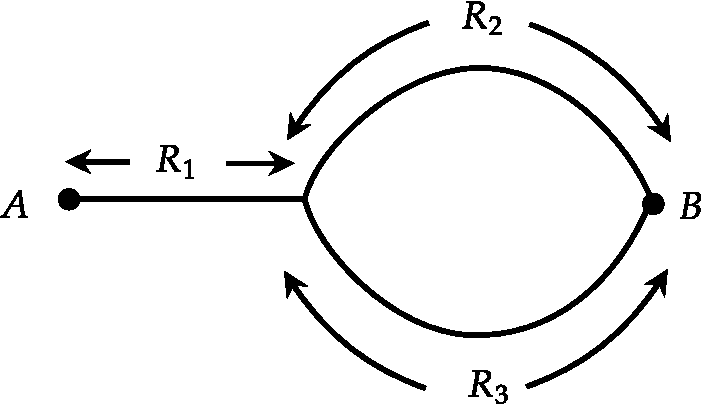
\includegraphics[height=3cm,width=5.5cm]{JEST-58-2019}
	\end{figure}
	\begin{tasks}(2)
		\task[\textbf{a.}]$\frac{8}{9}$
		\task[\textbf{b.}]$\frac{1}{3}$
		\task[\textbf{c.}]$\frac{4}{9}$
		\task[\textbf{d.}]$\frac{2}{3}$
	\end{tasks}
\end{enumerate}
 \colorlet{ocre1}{ocre!70!}
\colorlet{ocrel}{ocre!30!}
\setlength\arrayrulewidth{1pt}
\begin{table}[H]
	\centering
	\arrayrulecolor{ocre}
	\begin{tabular}{|p{1.5cm}|p{1.5cm}||p{1.5cm}|p{1.5cm}|}
		\hline
		\multicolumn{4}{|c|}{\textbf{Answer key}}\\\hline\hline
		\rowcolor{ocrel}Q.No.&Answer&Q.No.&Answer\\\hline
		1&\textbf{B} &2&\textbf{C}\\\hline 
		3&\textbf{D} &4&\textbf{A} \\\hline
		5&\textbf{A} &6&\textbf{A} \\\hline
		7&\textbf{D}&8&\textbf{9555(NAT)}\\\hline
		9&\textbf{C}&&\textbf{}\\\hline
		
	\end{tabular}
\end{table}

%\chapter{Practice set Solutions Differential Equations}
\begin{abox}
	Problem Set -1
\end{abox}
\begin{enumerate}[label=\color{ocre}\textbf{\arabic*.}]	
	\item Let $x_{1}(t)$ and $x_{2}(t)$ be two linearly independent solutions of the differential equation $\frac{d^{2} x}{d t^{2}}+2 \frac{d x}{d t}+f(t) x=0$ and let $w(t)=x_{1}(t) \frac{d x_{2}(t)}{d t}-x_{2}(t) \frac{d x_{1}(t)}{d t} .$ If $w(0)=1$, then $w(1)$ is given by
	{\exyear{ NET/JRF(DEC-2011)}}
			\begin{tasks}(4)
			\task[\textbf{A.}] 1
			\task[\textbf{B.}] $e^{2}$
			\task[\textbf{C.}]  $1 / e$
			\task[\textbf{D.}] $1 / e^{2}$
		\end{tasks}
			\begin{answer}
			\begin{align*}
			\intertext{$W(t)$ is Wronskian of D.E.}
			W&=e^{-\int \mathrm{Pdt}}=e^{-2 t} \Rightarrow W(1)\\&=e^{-2}\text{ since }P=2
			\end{align*}
			So the correct answer is \textbf{Option (D)}
		\end{answer}
\item Let $y(x)$ be a continuous real function in the range 0 and $2 \pi$, satisfying the inhomogeneous differential equation: $\sin x \frac{d^{2} y}{d x^{2}}+\cos x \frac{d y}{d x}=\delta\left(x-\frac{\pi}{2}\right)$ The value of $d y l d x$ at the point $x=\pi / 2$
{\exyear{NET/JRF (JUNE-2012)}}
\begin{tasks}(2)
	\task[\textbf{A.}] Is continuous
	\task[\textbf{B.}] Has a discontinuity of 3
	\task[\textbf{C.}] Has a discontinuity of $1 / 3$
	\task[\textbf{D.}] Has a discontinuity of 1
\end{tasks}
\begin{answer}
	\begin{align*}
	\text{After dividing by }\sin x, \frac{d^{2} y}{d x^{2}}+\cot x \frac{d y}{d x}&=\operatorname{cosec} x \cdot \delta\left(x-\frac{\pi}{2}\right)\\
	\text{Integrating both sides, }\frac{d y}{d x}+\int \cot x\left(\frac{d y}{d x}\right) d x&=\int \operatorname{cosec} x \delta\left(x-\frac{\pi}{2}\right) d x\\
	\frac{d y}{d x}+\cot x \cdot y-\int \operatorname{cosec}^{2} x \cdot y d x&=1\\
	\text{Using Dirac delta property: }\int f(x) \delta\left(x-x_{0}\right)&=f\left(x_{0}\right)\text{ (it lies with the limit).}\\
	\frac{d y}{d x}+y \cdot \frac{\cos x}{\sin x}-\int y \operatorname{cosec}^{2} x d x&=1,\text{ at }x=\pi ; \sin x=0 .\text{ So this is point of discontinuity.}
	\end{align*}
	So the correct answer is \textbf{Option (D)}
\end{answer}
\item The solution of the partial differential equation
$$
\frac{\partial^{2}}{\partial t^{2}} u(x, t)-\frac{\partial^{2}}{\partial x^{2}} u(x, t)=0
$$
satisfying the boundary conditions $u(0, t)=0=u(L, t)$ and initial conditions $u(x, 0)=\sin (\pi x / L)$ and $\left.\frac{\partial}{\partial t} u(x, t)\right|_{t=0}=\sin (2 \pi x / L)$ is
{\exyear{NET/JRF(JUNE-2013)}}
	\begin{tasks}(1)
		\task[\textbf{A.}] $\sin (\pi x / L) \cos (\pi t / L)+\frac{L}{2 \pi} \sin (2 \pi x / L) \cos (2 \pi t / L)$
		\task[\textbf{B.}] $2 \sin (\pi x / L) \cos (\pi t / L)-\sin (\pi x / L) \cos (2 \pi t / L)$
		\task[\textbf{C.}] $\sin (\pi x / L) \cos (2 \pi t / L)+\frac{L}{\pi} \sin (2 \pi x / L) \sin (\pi t / L)$
		\task[\textbf{D.}] $\sin (\pi x / L) \cos (\pi t / L)+\frac{L}{2 \pi} \sin (2 \pi x / L) \sin (2 \pi t / L)$
	\end{tasks}
	\begin{answer}
		\begin{align*}
		\frac{\partial^{2} u}{\partial t^{2}}-\frac{\partial^{2} u}{\partial x^{2}}&=0, u(x, 0)=\sin \frac{\pi x}{L}\text{ and }\left.\frac{\partial u}{\partial t}\right|_{t=0}=\sin \frac{2 \pi x}{L}\\
		\text{This is a wave equation}\\
		\text{So solution is given by }u(x, t)&=\sum_{n}\left(A_{n} \cos \frac{a n \pi t}{L}+B_{n} \sin \frac{a n \pi t}{L}\right) \sin \left(\frac{n \pi x}{L}\right)\\
		\text{with }A_{n}&=\frac{2}{L} \int_{0}^{L} f(x) \sin \frac{n \pi x}{L} d x, \\ B_{n}&=\frac{2}{a n \pi} \int_{0}^{L} g(x) \sin \frac{n \pi x}{L} d x\\
		\text{Comparing }a^{2} \frac{\partial^{2} u}{\partial t^{2}}&=\frac{\partial^{2} u}{\partial x^{2}},\text{ We have }a=1\text{ and }f(x)\\&=\sin \frac{\pi x}{L}, g(x)=\sin \frac{2 \pi x}{L}\\
		A_{n}&=\frac{2}{L} \int_{0}^{L} \sin \frac{\pi x}{L} \sin \frac{n \pi x}{L} d x \Rightarrow \frac{2}{L} \int_{0}^{L} \sin ^{2} \frac{\pi x}{L} d x\\&=\frac{2}{L} \int_{0}^{L}\left(\frac{1-\cos \frac{2 \pi x}{L}}{2}\right) d x=\frac{2}{L} \cdot \frac{L}{2}=1 (\text{let }\left.n=1\right)\\
		\text{Putting }n&=2, B_{n}=\frac{2}{a n \pi} \int_{0}^{L} \sin \frac{2 \pi x}{L} \cdot \sin \frac{n \pi x}{L} d x\\
		\Rightarrow \frac{2}{2 \pi} \int_{0}^{L} \sin ^{2} \frac{2 \pi x}{L} d x&=\frac{2}{2 \pi} \int_{0}^{L}\left(\frac{1-\cos \frac{4 \pi x}{L}}{2}\right) d x=\frac{2}{2 \pi} \cdot \frac{L}{2}=\frac{L}{2 \pi}
		\end{align*}
		So the correct answer is \textbf{Option (D)}
	\end{answer}
	\item The solution of the differential equation
	$$
	\frac{d x}{d t}=x^{2}
	$$
	with the initial condition $x(0)=1$ will blow up as $t$ tends to
	{\exyear{NET/JRF(JUNE-2013)}}
	\begin{tasks}(4)
		\task[\textbf{A.}] 1
		\task[\textbf{B.}] 2
		\task[\textbf{C.}] $\frac{1}{2}$
		\task[\textbf{D.}] $\infty$
	\end{tasks}
	\begin{answer}
		\begin{align*}
		\frac{d x}{d t}&=x^{2} \Rightarrow \int \frac{d x}{x^{2}}=\int d t \Rightarrow \frac{x^{-2+1}}{-2+1}\\&=t+C \Rightarrow \frac{-1}{x}=t+C\\
		\Rightarrow x(0)&=1 \Rightarrow \frac{-1}{1}=0+C \Rightarrow C=-1 \Rightarrow \frac{-1}{x}\\&=t-1 \Rightarrow x=\frac{1}{1-t}\text{ as }t \rightarrow 1, x\text{ blows up}
		\end{align*}
		So the correct answer is \textbf{Option (A)}
	\end{answer}
	\item Consider the differential equation
	$$
	\frac{d^{2} x}{d t^{2}}+2 \frac{d x}{d t}+x=0
	$$
	with the initial conditions $x(0)=0$ and $\dot{x}(0)=1$. The solution $x(t)$ attains its maximum value when $t$ is
	{\exyear{NET/JRF(JUNE-2014)}}
	\begin{tasks}(4)
		\task[\textbf{A.}] $1 / 2$
		\task[\textbf{B.}] 1
		\task[\textbf{C.}] 2
		\task[\textbf{D.}] $\infty$
	\end{tasks}
	\begin{answer}
		\begin{align*}
		\frac{d^{2} x}{d t^{2}}+2 \frac{d x}{d t}+x&=0 \Rightarrow m^{2}+2 m+1\\&=0 \Rightarrow(m+1)^{2}=0 \Rightarrow m=-1,-1\\
		\Rightarrow x&=\left(c_{1}+c_{2} t\right) e^{-t},\text{ since }x(0)\\&=0 \Rightarrow 0=c_{1} \Rightarrow x=c_{2} t e^{-t}\\
		\Rightarrow \dot{x}&=c_{2}\left[-t e^{-t}+e^{-t}\right]\\
		\text{Since }\dot{x}(0)&=1 \Rightarrow 1=c_{2} \Rightarrow x=t e^{-t}\\
		\text{For maxima or minima }\dot{x}&=0 \Rightarrow \dot{x}=-t e^{-t}+e^{-t}=0 \Rightarrow \dot{x}=e^{-t}(1-t)\\
		\Rightarrow e^{-t}&=0,1-t=0 \Rightarrow t=\infty, t=1\\
		\ddot{x}&=e^{-t}(-1)+(1-t) e^{-t}(-1)\\&=-e^{-t}+(t-1) e^{-t} \Rightarrow \ddot{x}(1)\\&=-e^{-1}+0 e^{-t}<0
		\end{align*}
		So the correct answer is \textbf{Option (B)}
	\end{answer}
	\item Consider the differential equation $\frac{d^{2} x}{d t^{2}}-3 \frac{d x}{d t}+2 x=0$. If $x=0$ at $t=0$ and $x=1$ at $t=1$, the value of $x$ at $t=2$ is
	{\exyear{NET/JRF(JUNE-2015)}}
	\begin{tasks}(4)
		\task[\textbf{A.}] $e^{2}+1$
		\task[\textbf{B.}] $e^{2}+e$
		\task[\textbf{C.}] $e+2$
		\task[\textbf{D.}] $2 e$
	\end{tasks}
	\begin{answer}
		\begin{align*}
		D^{2}-3 D+2&=0\\
		(D-1)(D-2)&=0 \Rightarrow D=1,2 \Rightarrow x=c_{1} e^{2 t}+c_{2} e^{t}\\
		\text{using boundary condition }x&=0, t=0 \Rightarrow c_{1}=-C_{2}\\
		\text{again using boundary condition }x&=1, t=1\\
		c_{2}&=\frac{1}{e-e^{2}}, c_{1}=\frac{1}{e^{2}-e} \Rightarrow x\\&=\frac{e^{2 t}}{e^{2}-e}+\frac{1}{e-e^{2}} e^{t}\\
		\text{again using }t&=2\text{ then }x=e^{2}+e
		\end{align*}
		So the correct answer is \textbf{Option (B)}
	\end{answer}
	\item  If $y=\frac{1}{\tanh (x)}$, then $x$ is
	{\exyear{NET/JRF(DEC-2015)}}
	\begin{tasks}(4)
		\task[\textbf{A.}] $\ln \left(\frac{y+1}{y-1}\right)$
		\task[\textbf{B.}] $\ln \left(\frac{y-1}{y+1}\right)$
		\task[\textbf{C.}]  $\ln \sqrt{\frac{y-1}{y+1}}$
		\task[\textbf{D.}]  $\ln \sqrt{\frac{y+1}{y-1}}$
	\end{tasks}
	\begin{answer}
		\begin{align*}
		y&=\frac{1}{\tanh x}\\
		y&=\frac{e^{x}+e^{-x}}{e^{x}-e^{-x}}=\frac{e^{2 x}+1}{e^{2 x}-1}\\
		y e^{2 x}-y&=e^{2 x}+1 \Rightarrow y e^{2 x}-e^{2 x}\\&=1+y \Rightarrow e^{2 x}(y-1)=(1+y)\\
		2 x&=\ln \left(\frac{y+1}{y-1}\right) \Rightarrow x=\frac{1}{2} \ln \left(\frac{y+1}{y-1}\right)\\&=\ln \left(\frac{y+1}{y-1}\right)^{\frac{1}{2}}
		\end{align*}
		So the correct answer is \textbf{Option (D)}
	\end{answer}
	\item The solution of the differential equation $\frac{d x}{d t}=2 \sqrt{1-x^{2}}$, with initial condition $x=0$ at $t=0$ is
	{\exyear{NET/JRF(DEC-2015)}}
	\begin{tasks}(2)
		\task[\textbf{A.}] $x=\left\{\begin{array}{ll}\sin 2 t, & 0 \leq t<\frac{\pi}{4} \\ \sinh 2 t, & t \geq \frac{\pi}{4}\end{array}\right.$
		\task[\textbf{B.}] $x=\left\{\begin{array}{cc}\sin 2 t, & 0 \leq t<\frac{\pi}{2} \\ 1, & t \geq \frac{\pi}{2}\end{array}\right.$
		\task[\textbf{C.}] $x=\left\{\begin{array}{cc}\sin 2 t, & 0 \leq t<\frac{\pi}{4} \\ 1, & t \geq \frac{\pi}{4}\end{array}\right.$
		\task[\textbf{D.}] $x=1-\cos 2 t, \quad t \geq 0$
	\end{tasks}
	\begin{answer}
		\begin{align*}
		\frac{d x}{d t}&=2 \sqrt{1-x^{2}}, \frac{d x}{\sqrt{1-x^{2}}}\\&=2 d t, \sin ^{-1} x=2 t+c, x=0, t=0 \\\text{ so, }c&=0 \Rightarrow x=\sin 2 t\\
		&\text{	$x$ should not be greater than 1 at $x=1$}\\
		1&=\sin 2 t, \quad \sin \frac{\pi}{2}=\sin 2 t, t=\frac{\pi}{4}\\
		\text{	So, }\quad x&=\left\{\begin{array}{ll}\sin 2 t, & 0 \leq t<\frac{\pi}{4} \\ 1, & t \geq \frac{\pi}{4}\end{array}\right.
		\end{align*}
		So the correct answer is \textbf{Option (C)}
	\end{answer}
	\item   The function $y(x)$ satisfies the differential equation $x \frac{d y}{d x}+2 y=\frac{\cos \pi x}{x}$. If $y(1)=1$, the value of $y(2)$ is
	{\exyear{NET/JRF(JUNE-2017)}}
	\begin{tasks}(4)
		\task[\textbf{A.}] $\pi$
		\task[\textbf{B.}] 1
		\task[\textbf{C.}] $1 / 2$
		\task[\textbf{D.}] $1 / 4$
	\end{tasks}
	\begin{answer}
		\begin{align*}
		\intertext{The given differential equation can be written as}
		\frac{d y}{d x}+\frac{2}{x} y&=\frac{\cos \pi x}{x^{2}}
		\intertext{This is a linear differential equation with Integrating factor $=e^{\int_{x}^{2} d x}=x^{2}$}
		\text{Hence }y . x^{2}&=\int x^{2} \cdot \frac{\cos \pi x}{x^{2}} d x+c \Rightarrow y\\&=\frac{\sin \pi x}{\pi x^{2}}+\frac{c}{x^{2}}\\
		\text{when }x&=1, y=1\text{ hence }c=1 \Rightarrow y\\&=\frac{\sin \pi x}{\pi x^{2}}+\frac{1}{x^{2}}\\
		\text{hence, when }x&=2, y=\frac{1}{4}
		\end{align*}
		So the correct answer is \textbf{Option (D)}
	\end{answer}
	\item   Consider the differential equation $\frac{d y}{d t}+a y=e^{-b t}$ with the initial condition $y(0)=0$. Then the Laplace transform $Y(s)$ of the solution $y(t)$ is
	{\exyear{NET/JRF(DEC-2017)}}
	\begin{tasks}(4)
		\task[\textbf{A.}] $\frac{1}{(s+a)(s+b)}$
		\task[\textbf{B.}] $\frac{1}{b(s+a)}$
		\task[\textbf{C.}] $\frac{1}{a(s+b)}$
		\task[\textbf{D.}] $\frac{e^{-a}-e^{-b}}{b-a}$
	\end{tasks}
	\begin{answer}
		\begin{align*}
		\text{Given }\frac{d y}{d t}+a y&=e^{-b t}
		\intertext{Taking Laplace transform of both sides}
		\text{	We obtain}\\
		L\left\{\frac{d y}{d t}\right\}+a L\{y(t)\}&=L\left\{e^{-b t}\right\} \Rightarrow s Y(s)-y(0)+a Y(s)=\frac{1}{s+b}\\
		\text{Since, }	y(0)&=0,\text{ we obtain}\\
		(s+a) Y(s)&=\frac{1}{s+b} \Rightarrow Y(s)=\frac{1}{(s+a)(s+b)}
		\end{align*}
		So the correct answer is \textbf{Option (A)}
	\end{answer}
	\item The number of linearly independent power series solutions, around $x=0$, of the second order linear differential equation $x \frac{d^{2} y}{d x^{2}}+\frac{d y}{d x}+x y=0$, is
	{\exyear{NET/JRF(DEC-2017)}}
	\begin{tasks}(1)
		\task[\textbf{A.}] 0 (this equation does not have a power series solution)
		\task[\textbf{B.}] 1
		\task[\textbf{C.}] 2
		\task[\textbf{D.}] 3
	\end{tasks}
	\begin{answer}
		So the correct answer is \textbf{Option (B)}
	\end{answer}
	\item The differential equation $\frac{d y(x)}{d x}=\alpha x^{2}$, with the initial condition $y(0)=0$, is solved using Euler's method. If $y_{E}(x)$ is the exact solution and $y_{N}(x)$ the numerical solution obtained using $n$ steps of equal length, then the relative error $\left|\frac{\left(y_{N}(x)-y_{E}(x)\right)}{y_{E}(x)}\right|$ is proportional to
	{\exyear{NET/JRF(DEC-2017)}}
	\begin{tasks}(4)
		\task[\textbf{A.}] $\frac{1}{n^{2}}$
		\task[\textbf{B.}] $\frac{1}{n^{3}}$
		\task[\textbf{C.}] $\frac{1}{n^{4}}$
		\task[\textbf{D.}] $\frac{1}{n}$
	\end{tasks}
	\begin{answer}
		\begin{align*}
		\frac{d y}{d x}&=\alpha x^{2}, y(0)=0\\
		y_{E}&=\frac{\alpha x^{3}}{3},\text{ but }x=n \hbar\\
		\text{Exact solution, }y_{E}&=\frac{\alpha n^{3} h^{3}}{3}\\
		\text{Numerically, }f(x, y)&=\alpha x^{2}\\
		\text{Euler's method, }y_{i}&=y_{i-1}+h f\left(x_{i-1}, y_{i-1}\right)\\
		y_{1}&=0, y_{2}=\alpha h^{3} \quad y_{3}=5 \alpha h^{3}\\
		y_{n}&=\frac{(n-1) n(2 n-1)}{6} \alpha h^{3}
		\intertext{Since, $0,5,14,30, \ldots$ different from square terms}
		\intertext{At, $x_{0}=0 \quad x_{1}=x_{0}+h=h \quad x_{2}=x_{0}+2 h=2 h \quad x_{3}=x_{0}+3 h=3 h$}
		x_{n-1}&=x_{0}+(n-1) h=(n-1) h .\text{ Now, }x_{n}=n h\\
		f\left(x_{0}, y_{0}\right)
		&=0, f\left(x_{1}, y_{1}\right)=\alpha h^{2}, f\left(x_{2}, y_{2}\right)=4 \alpha h^{2}\\
		f\left(x_{n-1}, y_{n-1}\right)&=\alpha(n-1)^{2} h^{2}\\
		\left|\frac{\left(y_{N}-y_{E}\right)}{y_{E}}\right|&=\left|\frac{\frac{(n-1) n(2 n-1) \alpha h^{3}}{6}-\frac{\alpha n^{3} h^{3}}{3}}{\frac{\alpha n^{3} h^{3}}{3}}\right|\\
		\text{By solving, }&\left|\frac{y_{N}-y_{E}}{y_{E}}\right| \propto \frac{1}{n}
		\end{align*}
		So the correct answer is \textbf{Option (D)}
	\end{answer}
	\item  Consider the following ordinary differential equation
	$$
	\frac{d^{2} x}{d t^{2}}+\frac{1}{x}\left(\frac{d x}{d t}\right)^{2}-\frac{d x}{d t}=0
	$$
	with the boundary conditions $x(t=0)=0$ and $x(t=1)=1 .$ The value of $x(t)$ at $t=2$ is
	{\exyear{NET/JRF(JUNE-2018)}}
	\begin{tasks}(4)
		\task[\textbf{A.}] $\sqrt{e-1}$
		\task[\textbf{B.}] $\sqrt{e^{2}+1}$
		\task[\textbf{C.}]  $\sqrt{e+1}$
		\task[\textbf{D.}] $\sqrt{e^{2}-1}$
	\end{tasks}
	\begin{answer}
		\begin{align*}
		\intertext{The given equation can be written as}
		\frac{1}{x} \frac{d}{d t}\left(x \frac{d x}{d t}\right)-\frac{d x}{d t}&=0 \Rightarrow \frac{d}{d t}\left(x \frac{d x}{d t}\right)-x \frac{d x}{d t}=0\\
		\text{putting }y&=x \frac{d x}{d t}\text{ gives}\\
		\frac{d y}{d t}-y&=0 \Rightarrow \ln y=t+\ln c_{1} \Rightarrow y=c_{1} e^{t}\\
		\intertext{Since $x \frac{d x}{d t}=c_{1} e^{t}$ hence by integrating}
		\frac{x^{2}}{2}&=c_{1} e^{t}+c_{2}\hspace{2cm}\text{(i)}
		\intertext{Using boundary conditions we obtain}
		c_{1}+c_{2}&=0\text{ and }c_{1} e+c_{2}=\frac{1}{2}
		\intertext{Solving these equations we obtain $c_{1}=\frac{1}{2(e-1)}$ and $c_{2}=-\frac{1}{2(e-1)}$}
		\text{Thus, }\frac{x^{2}}{2}&=\frac{1}{2(e-1)} e^{t}-\frac{1}{2(e-1)}\\
		\text{When }t&=2,\text{ we obtain, }\quad x^{2}=\frac{e^{2}}{(e-1)}-\frac{1}{(e-1)}\\&=\frac{\left(e^{2}-1\right)}{(e-1)}=e+1\\
		\text{Therefore}x(2)&=\sqrt{e+1}
		\end{align*}
		So the correct answer is \textbf{Option (C)}
	\end{answer}
	\item  In terms of arbitrary constants $A$ and $B$, the general solution to the differential equation $x^{2} \frac{d^{2} y}{d x^{2}}+5 x \frac{d y}{d x}+3 y=0$ is
	{\exyear{NET/JRF(DEC-2018)}}
	\begin{tasks}(4)
		\task[\textbf{A.}]  $y=\frac{A}{x}+B x^{3}$
		\task[\textbf{B.}] $y=A x+\frac{B}{x^{3}}$
		\task[\textbf{C.}] $y=A x+B x^{3}$
		\task[\textbf{D.}] $y=\frac{A}{x}+\frac{B}{x^{3}}$
	\end{tasks}
	\begin{answer}
		\begin{align*}
		\intertext{
			The given equation is Euler-Cauchy differential equation. The characteristic equation of}
		x^{2} \frac{d^{2} y}{d x^{2}}+5 x \frac{d y}{d x}+6 y&=0\\
		\text{is ,}m^{2}+4 m+6&=0 \Rightarrow m=-3 or m=-1\\
		\text{Thus, }y_{1}&=x^{-1}=\frac{1}{x}\text{ and }y_{2}=x^{2}=\frac{1}{x^{3}}
		\intertext{Therefore the general solution is}
		y&=\frac{A}{x}+\frac{B}{x^{3}}
		\end{align*}
		So the correct answer is \textbf{Option (D)}
	\end{answer}
	\item The solution of the differential equation $x \frac{d y}{d x}+(1+x) y=e^{-x}$ with the boundary condition $y(x=1)=0$, is
	{\exyear{NET/JRF(JUNE-2019)}}
	\begin{tasks}(4)
		\task[\textbf{A.}] $\frac{(x-1)}{x} e^{-x}$
		\task[\textbf{B.}] $\frac{(x-1)}{x^{2}} e^{-x}$
		\task[\textbf{C.}] $\frac{(1-x)}{x^{2}} e^{-x}$
		\task[\textbf{D.}] $(x-1)^{2} e^{-x}$
	\end{tasks}
	\begin{answer}
		\begin{align*}
		x \frac{d y}{d x}+(1+x) y&=e^{-x} \Rightarrow \frac{d y}{d x}+\frac{(1+x)}{x} y=\frac{e^{-x}}{x}\\
		\text{Let }p&=\frac{1+x}{x}\\
		I.F &=e^{\int p d x}=e^{\int\left(1+\frac{1}{x}\right) d x}=e^{x} \cdot e^{\ln x}=x e^{x}\\
		y \cdot x \cdot e^{x}&=\int \frac{e^{-x}}{x} \cdot x e^{x} d x+C \Rightarrow y \cdot x \cdot e^{x}=x+C\\
		y&=0\text{ at }x=1 \quad \Rightarrow C=-1 \quad \Rightarrow y \cdot x \cdot e^{x}\\&=x-1 \Rightarrow y=\left[\frac{x-1}{x}\right] e^{-x}
		\end{align*}
		So the correct answer is \textbf{Option (A)}
	\end{answer}
	\item The solution of the differential equation $\left(\frac{d y}{d x}\right)^{2}-\frac{d^{2} y}{d x^{2}}=e^{y}$, with the boundary conditions $y(0)=0$ and $y^{\prime}(0)=-1$, is
	{\exyear{NET/JRF(JUNE-2020)}}
	\begin{tasks}(4)
		\task[\textbf{A.}] $-\ln \left(\frac{x^{2}}{2}+x+1\right)$
		\task[\textbf{B.}] $-x \ln (e+x)$
		\task[\textbf{C.}] $-x e^{-x^{2}}$
		\task[\textbf{D.}]  $-x(x+1) e^{-x}$
	\end{tasks}
	\begin{answer}
		\begin{align*}
		\left(\frac{d y}{d x}\right)^{2}-\frac{d^{2} y}{d x^{2}}&=e^{y}\text{ put }y=\ln p\\
		\frac{d y}{d x}&=\frac{1}{p} \frac{d p}{d x} \Rightarrow \frac{d^{2} y}{d x^{2}}=\frac{d}{d x}\left(\frac{1}{p} \frac{d p}{d x}\right)\\&=\frac{1}{p} \frac{d^{2} p}{d x^{2}}-\frac{1}{p^{2}}\left(\frac{d p}{d x}\right)^{2}\\
		\text{Thus }&\left(\frac{1}{p} \frac{d p}{d x}\right)^{2}-\frac{1}{p} \frac{d^{2} p}{d x^{2}}+\frac{1}{p^{2}}\left(\frac{d p}{d x}\right)^{2}=p\\
		\frac{2}{p^{2}}\left(\frac{d p}{d x}\right)^{2}-\frac{1}{p} \frac{d^{2} p}{d x^{2}}&=p \Rightarrow \frac{2}{p^{3}}\left(\frac{d p}{d x}\right)^{2}-\frac{1}{p^{2}} \frac{d^{2} p}{d x^{2}}\\&=1 \Rightarrow \frac{1}{p^{2}} \frac{d^{2} p}{d x^{2}}-\frac{2}{p^{3}}\left(\frac{d p}{d x}\right)^{2}=-1\\
		&\Rightarrow \frac{d}{d x}\left(\frac{1}{p^{2}} \frac{d p}{d x}\right)=-1\\
		\text{Let }\frac{1}{p^{2}} \frac{d p}{d x}&=z \Rightarrow \frac{d z}{d x}=-1 \Rightarrow z=-x+c\\
		\text{Thus }\frac{1}{p^{2}} \frac{d p}{d x}&=-x+c \Rightarrow \int \frac{d p}{p^{2}}=\int(-x+c) d x\\
		-\frac{1}{p}&=-\frac{x^{2}}{2}+c x+d \Rightarrow p=\frac{1}{\frac{x^{2}}{2}-c x-d}\\
		y&=\ln p=\ln \left(\frac{1}{\frac{x^{2}}{2}-c x-d}\right)=\ln \left(\frac{x^{2}}{2}-c x-d\right)\\
		y(0)&=0 \Rightarrow y(0)=-\ln (-d) \Rightarrow d=-1\\
		y&=-\ln \left(\frac{x^{2}}{2}-c x+1\right)\\
		y^{\prime}(x)&=-\frac{1}{\left(\frac{x^{2}}{2}-c x+1\right)}(x-c), \quad y^{\prime}(0)\\&=-1 \Rightarrow-\frac{(-c)}{1}=c=-1, \quad y=-\ln \left(\frac{x^{2}}{2}+x+1\right)
		\end{align*}
		So the correct answer is \textbf{Option (A)}
	\end{answer}
\end{enumerate}
 \colorlet{ocre1}{ocre!70!}
\colorlet{ocrel}{ocre!30!}
\setlength\arrayrulewidth{1pt}
\begin{table}[H]
	\centering
	\arrayrulecolor{ocre}
	\begin{tabular}{|p{1.5cm}|p{1.5cm}||p{1.5cm}|p{1.5cm}|}
		\hline
		\multicolumn{4}{|c|}{\textbf{Answer key}}\\\hline\hline
		\rowcolor{ocrel}Q.No.&Answer&Q.No.&Answer\\\hline
		1&\textbf{D} &2&\textbf{D}\\\hline 
		3&\textbf{D} &4&\textbf{A} \\\hline
		5&\textbf{B} &6&\textbf{B} \\\hline
		7&\textbf{D}&8&\textbf{C}\\\hline
		9&\textbf{D}&10&\textbf{A}\\\hline
		11&\textbf{B} &12&\textbf{D}\\\hline
		13&\textbf{C}&14&\textbf{D}\\\hline
		15&\textbf{A}&16&\textbf{A} \\\hline
		
	\end{tabular}
\end{table}
\newpage
\begin{abox}
	Problem Set -2
\end{abox}
\begin{enumerate}[label=\color{ocre}\textbf{\arabic*.}]
	\item  The solution of the differential equation for $y(t): \frac{d^{2} y}{d t^{2}}-y=2 \cosh (t)$, subject to the initial conditions $y(0)=0$ and $\left.\frac{d y}{d t}\right|_{t=0}=0$, is
	{\exyear{GATE 2010}}
	\begin{tasks}(2)
		\task[\textbf{A.}] $\frac{1}{2} \cosh (t)+t \sinh (t)$
		\task[\textbf{B.}] $-\sinh (t)+t \cosh (t)$
		\task[\textbf{C.}] $t \cosh (t)$
		\task[\textbf{D.}] $t \sinh (t)$
	\end{tasks}
	\begin{answer}
		\begin{align}
		\text{	For C.F } \left(D^{2}-1\right) y&=0 \Rightarrow m=\pm 1 \Rightarrow C . F .\notag\\&=C_{1} e^{t}+C_{2} e^{-t}\notag\\
		P.I. &=\frac{1}{D^{2}-1}(2 \cosh t)=\frac{1}{D^{2}-1} 2\left(\frac{e^{t}+e^{-t}}{2}\right)\notag\\&=\frac{1}{D^{2}-1}\left(e^{t}\right)+\frac{1}{D^{2}-1}\left(e^{-t}\right)\notag\\&=\frac{t}{2} e^{t}+\frac{t}{2}\left(-e^{-t}\right)\notag\\
		\Rightarrow y&=C_{1} e^{t}+C_{2} e^{-t}+\frac{t}{2} e^{t}-\frac{t}{2} e^{-t}\notag\\
		\text{As, }y(0)&=0 \Rightarrow C_{1}+C_{2}=0\label{math01}\\
		\frac{d y}{d t}&=C_{1} e^{t}-C_{2} e^{-t}+\frac{t}{2} e^{t}+\frac{1}{2} e^{t}+\frac{t}{2} e^{-t}-\frac{1}{2} e^{-t}\notag\\
		\text{Also, }\left.\frac{d y}{d t}\right|_{t=0}&=0 \Rightarrow C_{1}-C_{2}+0+\frac{1}{2}+0-\frac{1}{2}=0 \Rightarrow C_{1}-C_{2}=0\label{math02}\\
		\text{From equation (\ref{math01}) and (\ref{math02}),}\notag\\
		C_{1}&=0, C_{2}=0\notag\\
		\text{Thus }y&=\frac{t}{2} e^{t}-\frac{t}{2} e^{-t} \Rightarrow y=t \sinh t\notag
		\end{align}
		So the correct answer is \textbf{Option (D)}
	\end{answer}
	\item The solutions to the differential equation $\frac{d y}{d x}=-\frac{x}{y+1}$ are a family of
	{\exyear{GATE 2011}}
	\begin{tasks}(1)
		\task[\textbf{A.}] Circles with different radii
		\task[\textbf{B.}] Circles with different centres
		\task[\textbf{C.}]  Straight lines with different slopes
		\task[\textbf{D.}]  Straight lines with different intercepts on the $y$-axis
	\end{tasks}
	\begin{answer}
		\begin{align*}
		\frac{d y}{d x}&=-\frac{x}{y+1} \Rightarrow x d x+y d y+d y\\&=0 \Rightarrow \frac{x^{2}}{2}+\frac{y^{2}}{2}+y\\&=C_{1} \Rightarrow x^{2}+y^{2}+2 y\\&=2 C_{1}
		\Rightarrow(x-0)^{2}+(y+1)^{2}\\&=2 C_{1}+1=C
		\intertext{which is a family of circles with different radii.}
		\end{align*}
		So the correct answer is \textbf{Option (A)}
	\end{answer}
	\item The solution of the differential equation $\frac{d^{2} y}{d t^{2}}-y=0$, subject to the boundary conditions $y(0)=1$ and $y(\infty)=0$ is
	{\exyear{GATE 2014}}
	\begin{tasks}(4)
		\task[\textbf{A.}] $\cos t+\sin t$
		\task[\textbf{B.}] $\cosh t+\sinh t$
		\task[\textbf{C.}] $\cos t-\sin t$
		\task[\textbf{D.}]  $\cosh t-\sinh t$
	\end{tasks}
	\begin{answer}
		\begin{align*}
		D^{2}-1&=0 \Rightarrow D=\pm 1 \Rightarrow y(t)\\&=c_{1} e^{t}+c_{2} e^{-t}
		\intertext{Applying boundary condition,}
		y(0)&=1 \Rightarrow 1=c_{1}+c_{2}\text{ and }y(\infty)\\&=0 \Rightarrow 0=c_{1} e^{\infty}+c_{2} e^{-\infty} \Rightarrow c_{1}\\&=0, c_{2}=1\\
		\Rightarrow y(t)&=e^{-t} \Rightarrow y(t)=\cosh t-\sinh \ t
		\end{align*}
		So the correct answer is \textbf{Option (D)}
	\end{answer}
	\item  A function $y(z)$ satisfies the ordinary differential equation $y^{\prime \prime}+\frac{1}{z} y^{\prime}-\frac{m^{2}}{z^{2}} y=0$, where\\
	$m=0,1,2,3, \ldots . .$ Consider the four statements P, Q, R, S as given below.\\
	$\mathrm{P}: z^{m}$ and $z^{-m}$ are linearly independent solutions for all values of $m$\\
	Q: $z^{m}$ and $z^{-m}$ are linearly independent solutions for all values of $m>0$\\
	$\mathrm{R}$ : $\ln z$ and 1 are linearly independent solutions for $m=0$\\
	S: $z^{m}$ and $\ln z$ are linearly independent solutions for all values of $m$\\
	The correct option for the combination of valid statements is
	{\exyear{GATE 2015}}
	\begin{tasks}(4)
		\task[\textbf{A.}] P, R and S only
		\task[\textbf{B.}]  P and R only
		\task[\textbf{C.}] $\mathrm{Q}$ and $\mathrm{R}$ only
		\task[\textbf{D.}] $\mathrm{R}$ and $\mathrm{S}$ only
	\end{tasks}
	\begin{answer}
		\begin{align*}
		y^{\prime \prime}+\frac{1}{z} y^{\prime}-\frac{m^{2}}{z^{2}} y&=0 \Rightarrow z^{2} y^{\prime \prime}+z y^{\prime}-m^{2} y\\&=0, m=0,1,2,3, \ldots, \quad z=e^{x}, D=\frac{d}{d x}\\
		\text{	If }m&=0 ; \quad z^{2} y^{\prime \prime}+z y^{\prime}=0,[D(D-1)+D] y\\&=0 \Rightarrow\left[D^{2}-D+D\right] y=0\\
		D^{2} y&=0 \Rightarrow y=c_{1}+c_{2} x \Rightarrow y\\&=c_{1}+c_{2} \ln z \quad \text{( $R$ is correct)}\\
		\text{And if }m &\neq 0, m>0,\text{ then }m \neq 0,\text{ then }\left(D^{2}-m^{2}\right) y\\&=0 \Rightarrow D=\pm m\\
		y&=c_{1} e^{m x}+c_{2} e^{-m x}=c_{1} e^{m \log z}+c_{2} e^{-m \log z}\\&=c_{1} z^{m}+c_{2} z^{-m}\\
		\text{or if }m &\neq 0, m>0,\text{ then}\\
		y&=c_{1} \cosh (m \log (z))+i c_{2} \sinh (m \log (x)), \quad m>0
		\end{align*}
		So the correct answer is \textbf{Option (C)} 
	\end{answer}
	\item Consider the linear differential equation $\frac{d y}{d x}=x y$. If $y=2$ at $x=0$, then the value of $y$ at $x=2$ is given by
	{\exyear{GATE 2016}}
	\begin{tasks}(4)
		\task[\textbf{A.}]  $e^{-2}$
		\task[\textbf{B.}] $2 e^{-2}$
		\task[\textbf{C.}] $e^{2}$
		\task[\textbf{D.}]  $2 e^{2}$
	\end{tasks}
	\begin{answer}
		\begin{align*}
		\frac{d y}{d x}&=x y \Rightarrow \frac{1}{y} d y=x d x \Rightarrow \ln y\\&=\frac{x^{2}}{2}+\ln c \Rightarrow y=c e^{x^{2} / 2}\\
		\text{If }y&=2\text{ at }x=0 \Rightarrow c=2 \Rightarrow y=2 e^{x^{2} / 2}\\
		\text{	The value of $y$ at }x&=2\text{ is given by }y=2 e^{2}
		\end{align*}
		So the correct answer is \textbf{Option (D)}
	\end{answer}
	\item Consider the differential equation $\frac{d y}{d x}+y \tan (x)=\cos (x)$. If $y(0)=0, y\left(\frac{\pi}{3}\right)$ is ............... (up to two decimal places)
	{\exyear{GATE 2017}}
	\begin{answer}
		\begin{align*}
		\intertext{The given differential equation is a linear differential equation of the form}
		\frac{d y}{d x}+p(x) y&=\cos x\\
		\text{	Integrating factor }&=e^{\int p(x) d x}\\
		\text{Thus integrating factor }&=e^{\int \tan x d x}\\
		\Rightarrow I \cdot F&=e^{\ln \sec x}=\sec x
		\intertext{Thus the general solution of the given differential equation is}
		y \cdot \sec x&=\int \sec x \cdot \cos x d x+c\\
		\Rightarrow y \sec x&=x+c\\
		\text{It is given that }y(0)&=0 \Rightarrow 0 \cdot \sec 0=0+c \Rightarrow c=0
		\intertext{Thus the solution satisfying the given condition is}
		y \sec x&=x \Rightarrow y=\frac{x}{\sec x}\\
		\text{Thus the value of }&y\left(\frac{\pi}{3}\right)\text{ is}\\
		y&=\frac{\pi / 3}{\sec \pi / 3}=\frac{\pi / 3}{2}=\frac{\pi}{6}=0 \cdot 52
		\end{align*}
	\end{answer}
	\item Given
	$$
	\frac{d^{2} f(x)}{d x^{2}}-2 \frac{d f(x)}{d x}+f(x)=0
	$$
	and boundary conditions $f(0)=1$ and $f(1)=0$, the value of $f(0.5)$ is --------(up
	to two decimal places).
	{\exyear{GATE 2018}}
	\begin{answer}
		\begin{align}
		\frac{d^{2} f(x)}{d x^{2}}-2 \frac{d f(x)}{d x}+f(x)&=0\notag\\
		\text{Auxiliary equation is,}\notag\\
		\left(m^{2}-2 m+1\right)&=0 \Rightarrow(m-1)^{2}\notag\\&=0 \Rightarrow m=1,1\notag\\
		\text{Hence, the solution is}\notag\\
		f(x)&=\left(c_{1}+c_{2} x\right) e^{x}\notag\\
		\text{using boundary condition,}\notag\\
		f(0)&=c_{1} e^{0} \Rightarrow c_{1}=1 \label{ma 03}\\
		f(1)&=\left(c_{1}+c_{2}\right) e=0 \label{ma 04}\\
		\text{	From (\ref{ma 03}) and (\ref{ma 04}), }c_{2}&=-1 \label{ma 05}\notag\\
		\text{Hence, }f(x)&=(1-x) e^{x} \Rightarrow f(0.5)\notag\\&=(1-0.5) e^{0.5}=0.81\notag
		\end{align}
	\end{answer}
	\item  For the differential equation $\frac{d^{2} y}{d x^{2}}-n(n+1) \frac{y}{x^{2}}=0$, where $n$ is a constant, the product of
	its two independent solutions is
	{\exyear{GATE 2019}}
	\begin{tasks}(4)
		\task[\textbf{A.}] $\frac{1}{x}$
		\task[\textbf{B.}] $x$
		\task[\textbf{C.}] $x^{n}$
		\task[\textbf{D.}] $\frac{1}{x^{n+1}}$
	\end{tasks}
	\begin{answer}
		So the correct answer is \textbf{Option (B)}
	\end{answer}
\end{enumerate}









%----------------------------------------------------------------------------------------
%	INDEX
%----------------------------------------------------------------------------------------

\cleardoublepage % Make sure the index starts on an odd (right side) page
\phantomsection
\setlength{\columnsep}{0.75cm} % Space between the 2 columns of the index
\addcontentsline{toc}{chapter}{\textcolor{ocre}{Index}} % Add an Index heading to the table of contents


%----------------------------------------------------------------------------------------

\end{document}
